\documentclass[openany]{book}


\usepackage{parskip,wrapfig,graphicx,subcaption}
\usepackage{hyperref}
\usepackage{fullpage}

\hypersetup{
    colorlinks,
    citecolor=black,
    filecolor=black,
    linkcolor=black,
    urlcolor=blue
}




\title{Curta Type 3DP Build Manual}
\date{}

\begin{document}
\maketitle

\tableofcontents

\chapter{Introduction}
This build manual is an attempt to describe the detailed and extensively manual process by which
I build my 3D printed Curta Calculators.


\section{Change Log}

\section{Safety Warning}


\section{Tools and Parts}
All tools, parts, quantities, and recommended print settings are described in the Bill of Materials. In this build manual I assume support material has already been removed and basic clean-up of the parts has been completed.



\section{A Note About Fitting Parts}
As you already know, a Fused Deposition Modeling (FDM) or Fused Filament Fabrication (FFF) 3D Printer prints parts by extruding plastic in layers. Each layer has a rounded shape which means a straight vertical wall is not actually straight. It is composed of multiple rounded layers of plastic that approximate a straight vertical wall. Friction will wear the rounded edges faster than a truly flat surface. This is a problem as it alters how the pieces will fit together.

\begin{figure}[!ht]
	\centering
	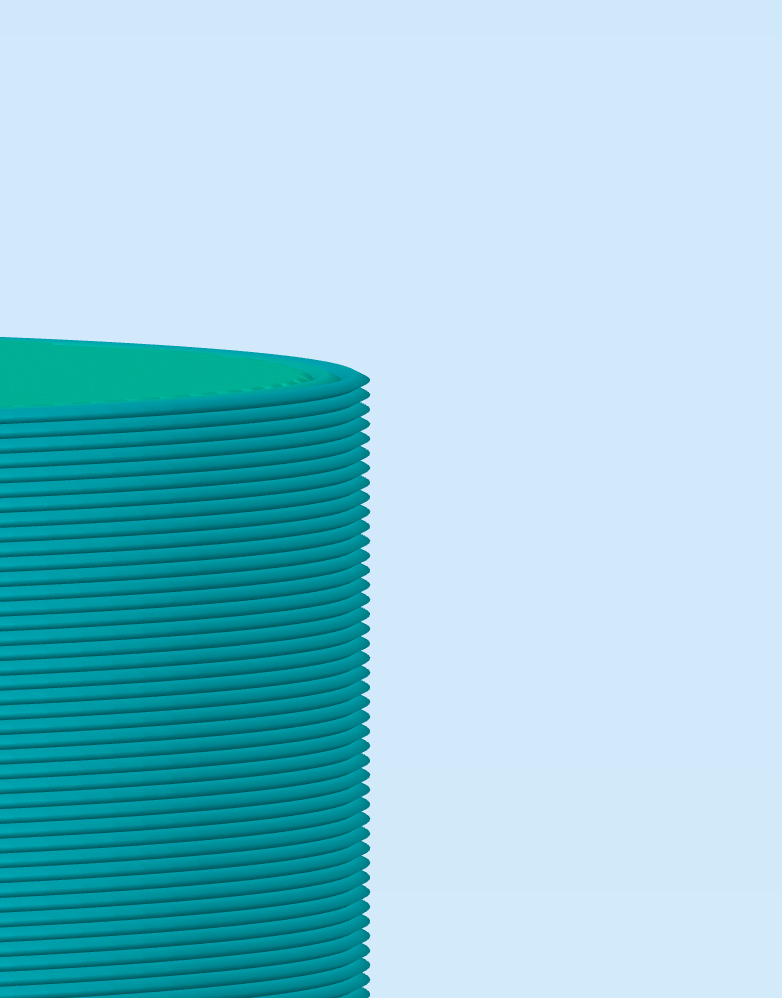
\includegraphics[width=.25\textwidth]{images/image12.png}
	\caption{Layer Lines}
	\label{fig:layerlines}
\end{figure}

I first encountered this issue during the planning phase of this project while running some tests to determine what tolerances I needed in order to get the various mechanical fits that the engineering drawings call for.

To combat this problem, I designed the various parts to fit too tightly. After some filing / sanding, they fit perfectly and lack high areas that wear away quickly. Unfortunately, this also means that each part has to be filed and tested against its mating parts for fit repeatedly until the desired fit is achieved. It is tedious and time-consuming, but necessary for reliable function.

I will describe the fit needed for each part as I go.


\section{Preparing and Painting External Facing Parts}
In order to save space and avoid repeating myself, instead of describing the details about how to paint each and every part, I will describe my process once here and make any particular notes I feel necessary for each part in appropriate spots throughout the manual.

The preparation for painting is done in two steps:
\begin{enumerate}
\item Sand to reduce the 3D print layer lines
\item Fill to eliminate imperfections and remaining layer lines
\end{enumerate}
The result should leave a perfect surface where it is indistinguishable that 3D printing was the manufacturing process.

For step one, I used a 220 grit sandpaper to make the parts as smooth as possible, eliminating layer lines. Many of the surfaces of the Curta are smooth, cylindrical surfaces, but a few are knurled. The knurled surfaces use a cut that is around 90 degrees, so the edge of a block of wood with sandpaper wrapped around it should suffice. For other small surfaces, needle files and other small tools can be helpful.

For step two, on larger imperfections I used a \href{http://amzn.to/2nBwh0R}{bondo putty} followed by sanding with 320-400 grit sandpaper. On smaller flaws I used a \href{http://amzn.to/2nwQNPs}{filler primer spray paint} followed by sanding with 320-400 grit sandpaper.

\begin{figure}[!ht]
	\centering
	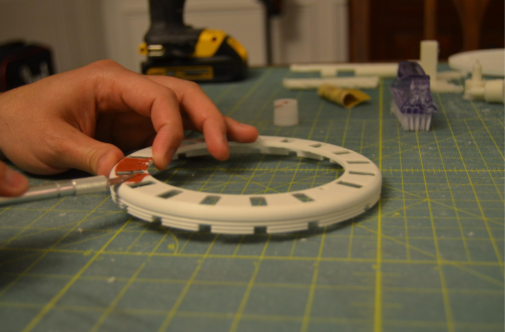
\includegraphics[width=.75\textwidth]{images/image13.png}
	\caption{Applying Bondo as a filler to repair defects}
	\label{fig:image13}	
\end{figure}


After getting a nice smooth surface to work from, follow the instructions on your spray paint to get light, but even coats. If accuracy is desired, the portions of the Curta between the knurled top and bottom are painted in a flat paint while the areas not between the knurled portions including the knurled sections themselves is glossy. To accomplish this, I used a flat black paint and used a matte clear coat for areas between the knurled portions or glossy clear coat for the rest. I used a clear coat on all paint to help protect it.
\begin{figure}[!ht]
	\centering
	\begin{subfigure}{.4\textwidth}
		\centering
		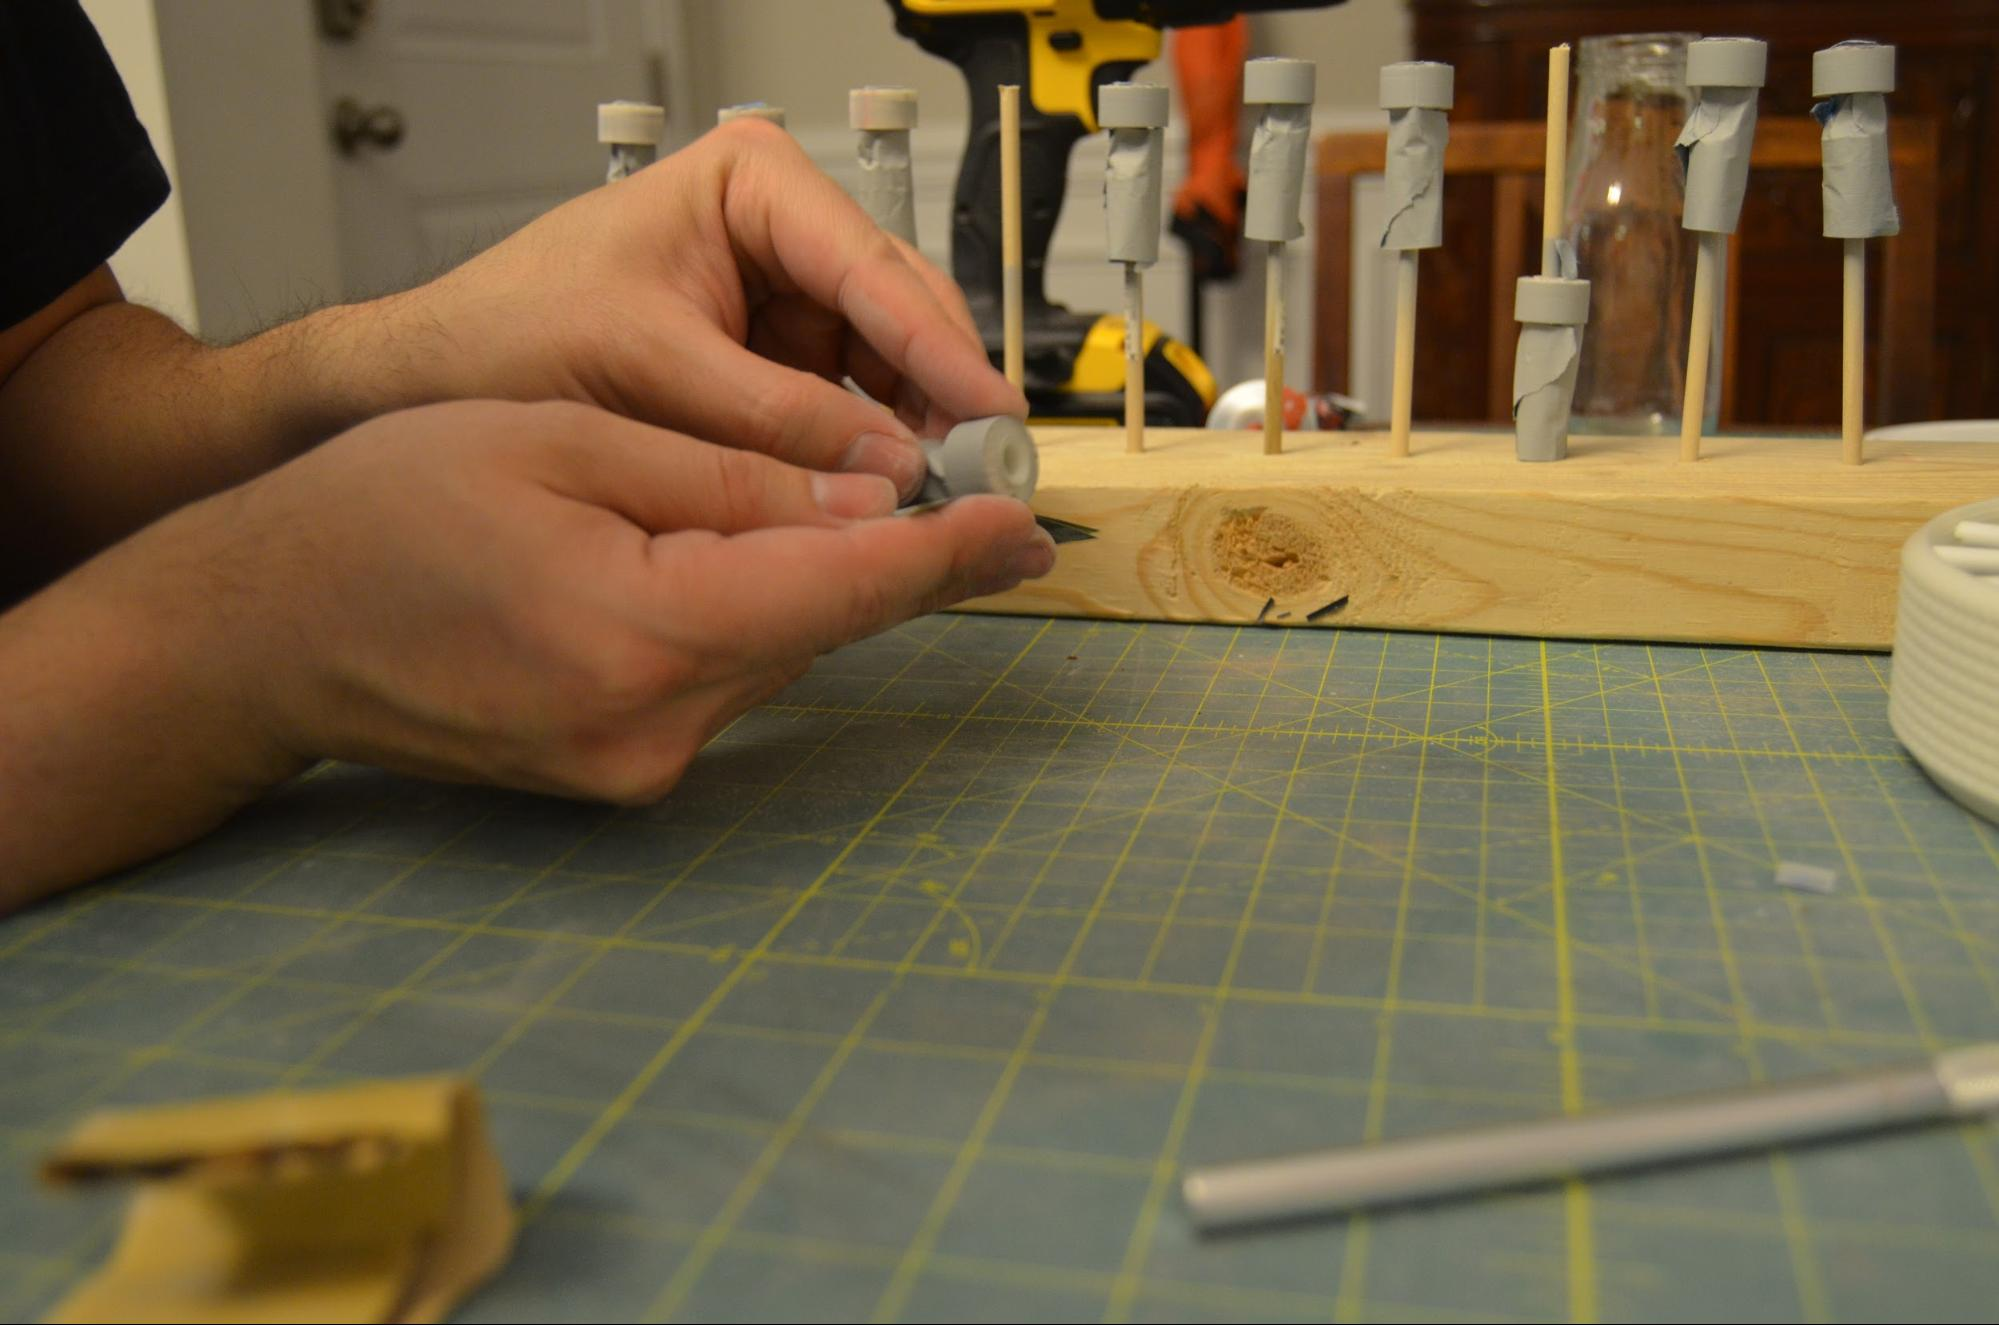
\includegraphics[width=.95\textwidth]{images/image42.jpg}
		%\caption{Image 42}
		\label{fig:image42}	
	\end{subfigure}
	\begin{subfigure}{.4\textwidth}
		\centering
		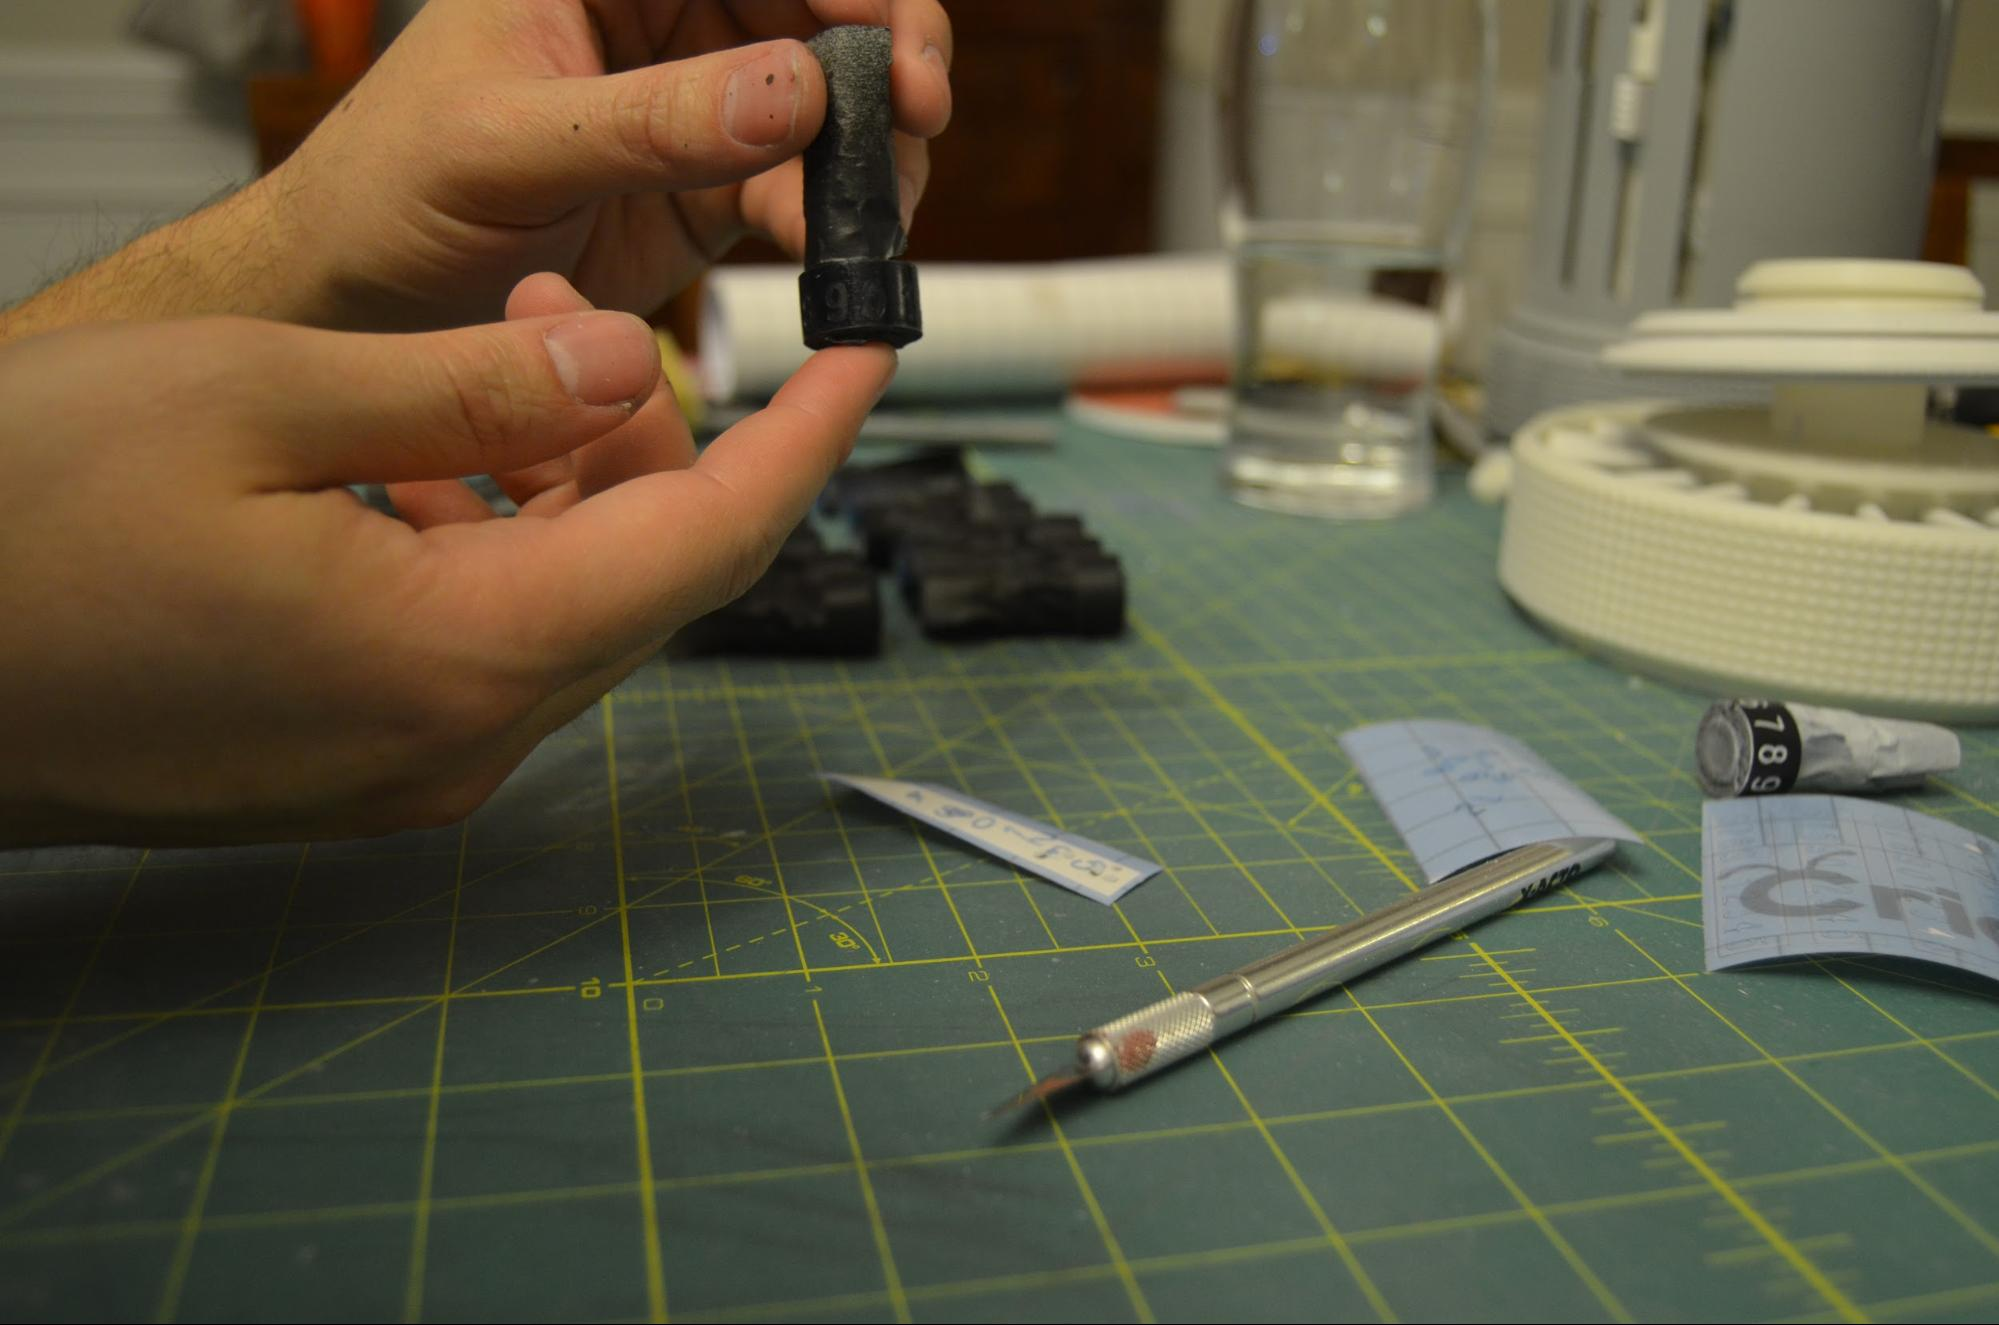
\includegraphics[width=.95\textwidth]{images/image34.jpg}
		%\caption{Image 34}
		\label{fig:image34}	
	\end{subfigure}
	\caption{Preparing Results Dials for Lettering and Numbering}
\end{figure}


Lettering and numbering was done with stencils cut using a home cutting machine (such as silhouette or cricut machines). Cut the stencils (files are provided on the thingiverse thing) using your machine or use someone else’s. Apply the stencils to your parts, working out any air bubbles. Remove portions of the stencils that should be painted. Spray a light coat of the background color (black if following the normal Curta paint scheme) to help seal any gaps or air bubbles that couldn’t be worked out of the stencils, let that dry for as long as the directions specify between coats, then spray a coat of the foreground color (white). Once that is dry, slowly peel the stencil away. The foreground color should be done in light coats to prevent the lettering from standing out too far from the background. Spray the clear coat on after the lettering or numbering to protect both the background and foreground.


\begin{figure}[!ht]
	\centering
	\begin{subfigure}{.4\textwidth}
		\centering
		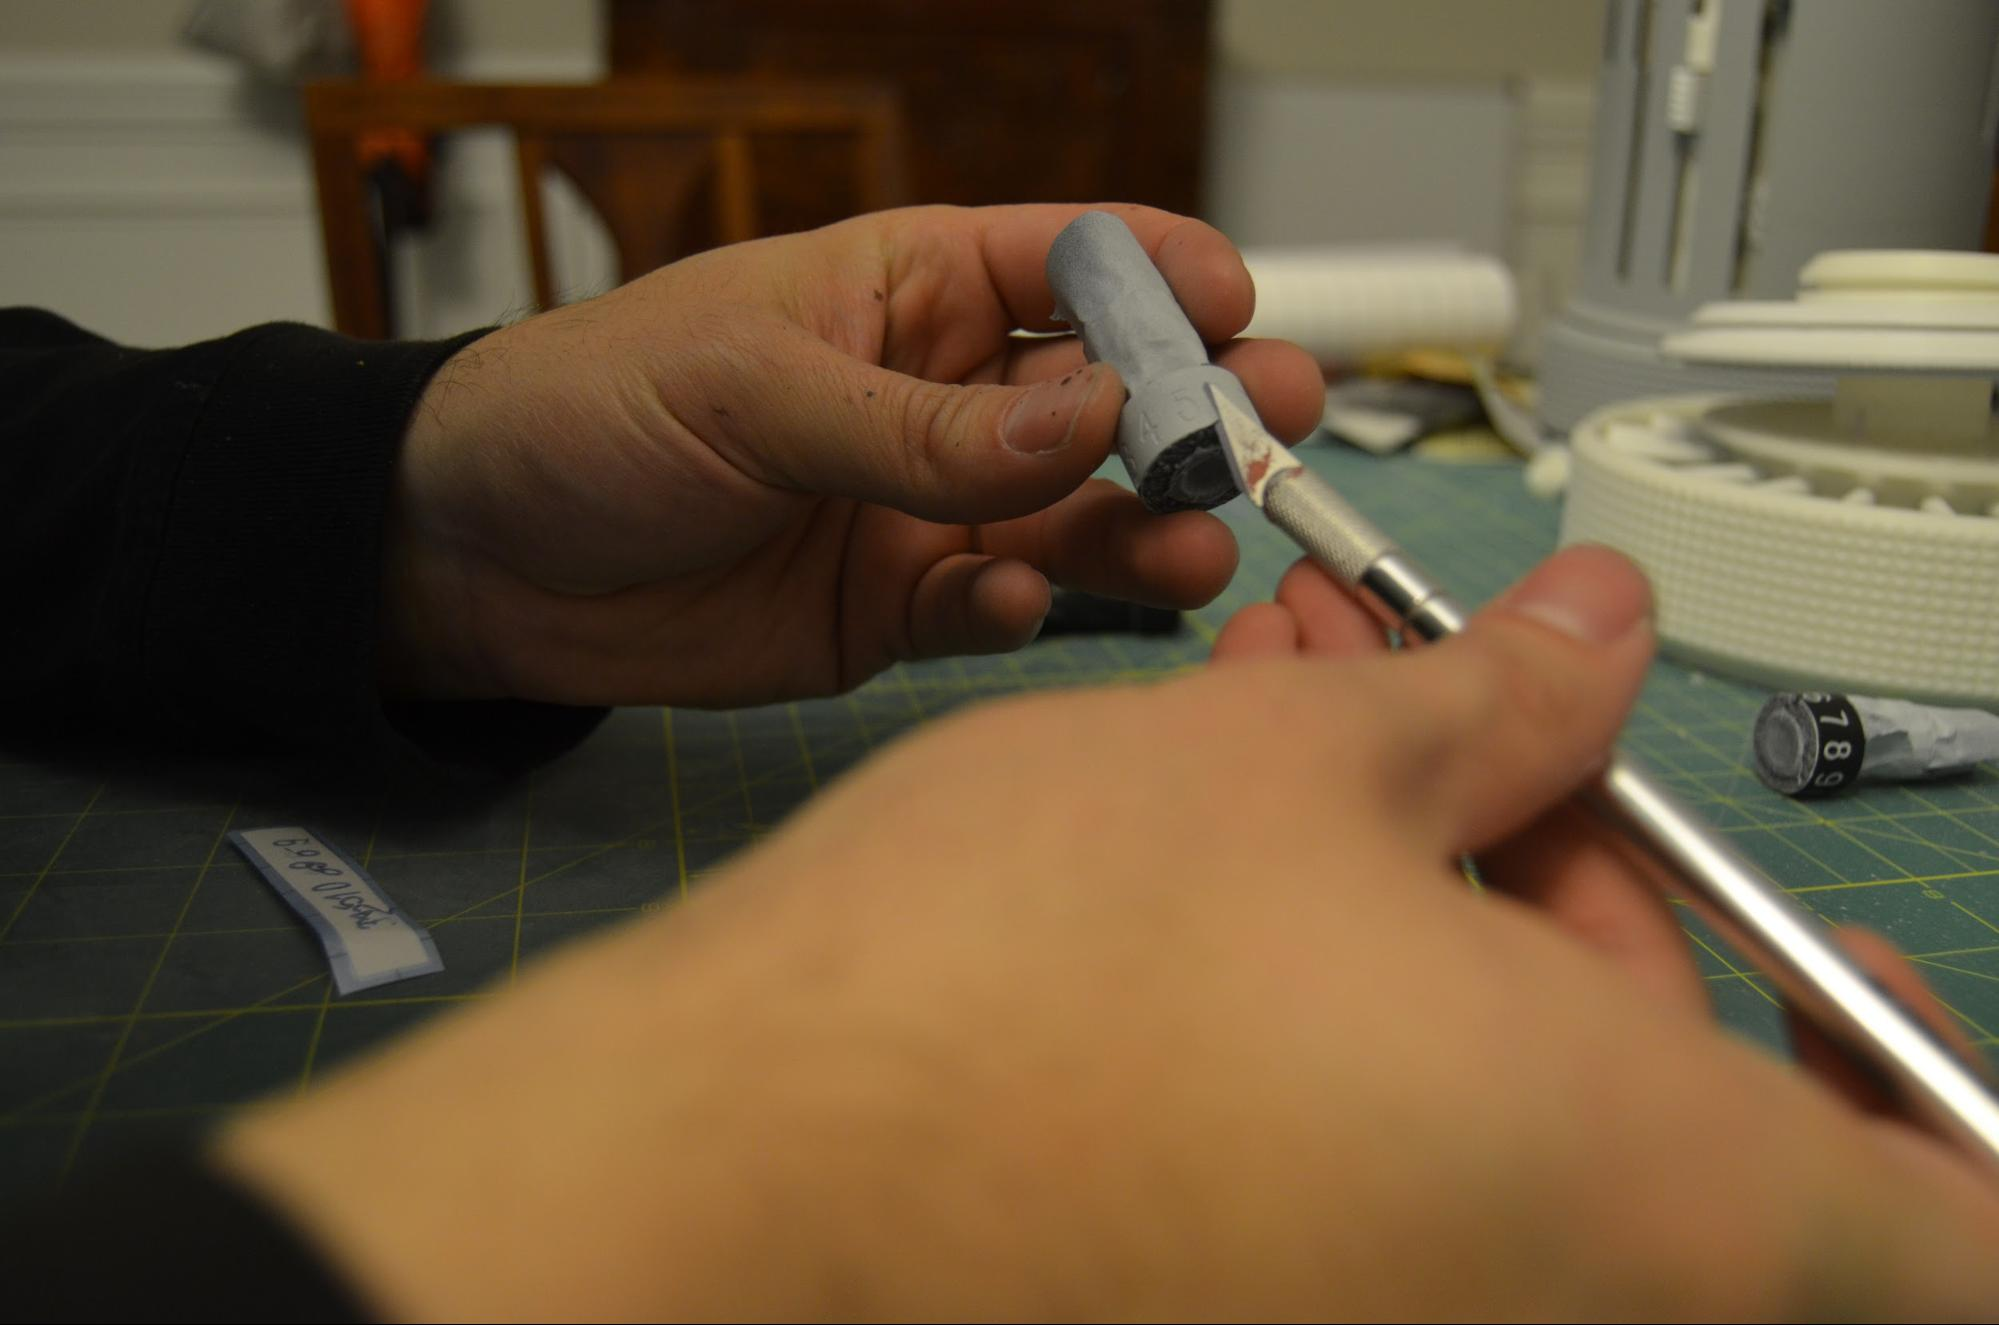
\includegraphics[width=.95\textwidth]{images/image36.jpg}
		%\caption{Image 36}
		\label{fig:image36}	
	\end{subfigure}
	\begin{subfigure}{.4\textwidth}
		\centering
		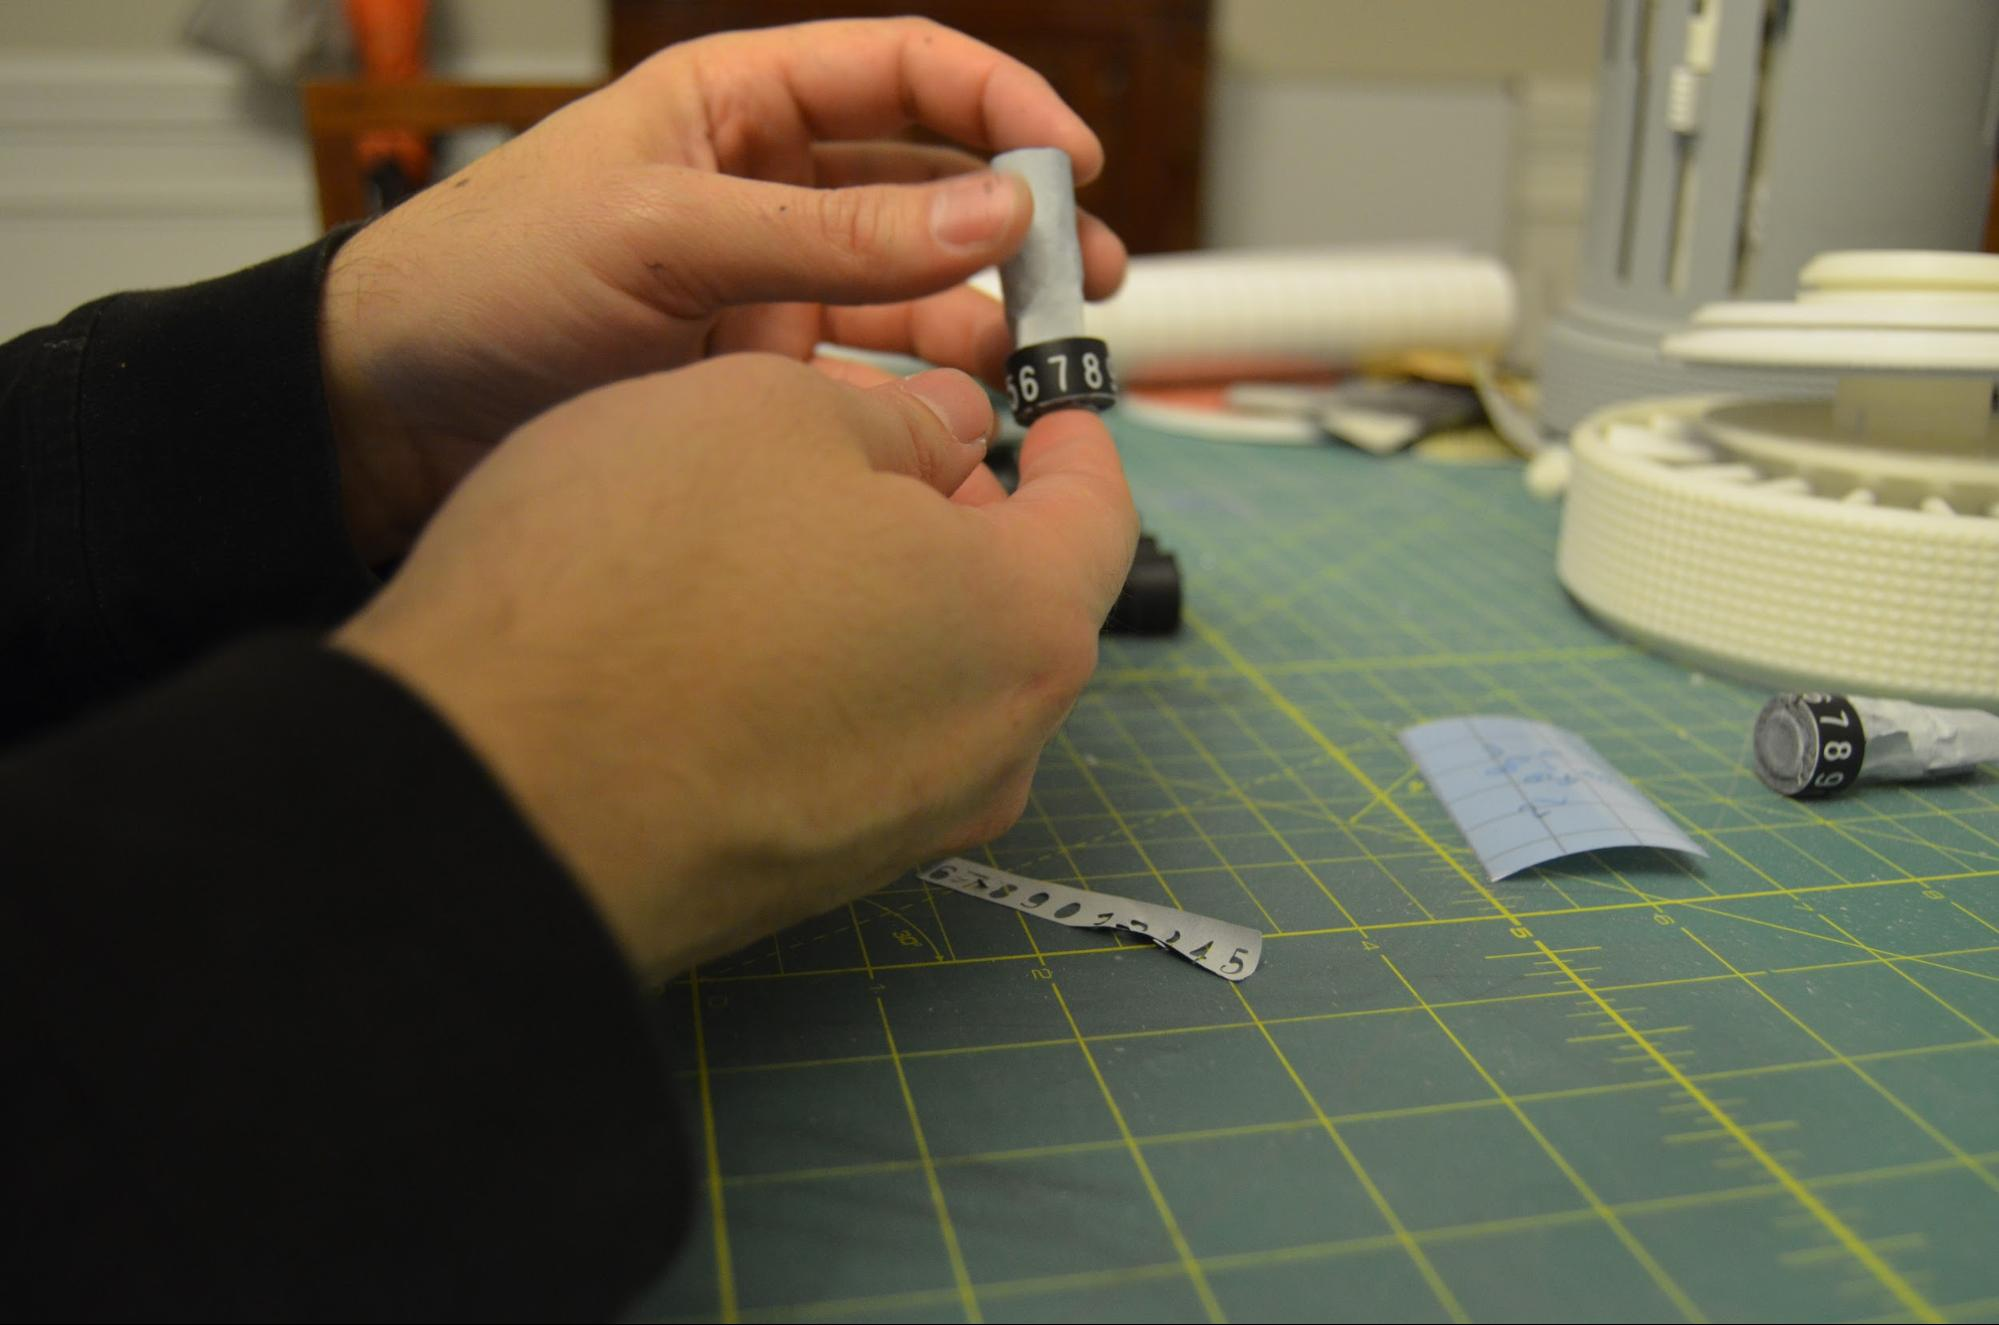
\includegraphics[width=.95\textwidth]{images/image35.jpg}
		%\caption{Image 35}
		\label{fig:image35}	
	\end{subfigure}
	\caption{Final Lettering and Numbering}
\end{figure}


\chapter{Preparing Main Casting and Bearing Plate}
\section{Parts Required}

\begin{table}[!ht]
	\centering
	\begin{tabular}{clc}
		Part Number & Part Name & Quantity (if $>1$) \\ \hline
		2 & Selector Shaft Top & \\
		13 & Main Shaft Bottom & \\
		26 & Support Columns (Frame Support) & \\
		28,29,30,31 & Transmission Axles & \\
		57 & Bearing Plate & 
	\end{tabular}
\end{table}

\section{Tools Required}

\begin{itemize}
	\item Needle Files
	\item M3, M4, M5 taps
	\item Sandpaper
	\item PTFE spray lubricant
\end{itemize}

\section{Process}

The main casting and bearing plate need to have the holes in them fit properly before assembly starts or little bits of plastic will end up in other parts. The following is a list of the things that should be fit:
\begin{itemize}
\item The main axle bottom should fit into the center of the bearing plate and turn smoothly / freely.
\item The support columns should press into the bearing plate and main casting somewhat easily and fit snugly.
\item The transmission axles should slide into and spin smoothly / freely in the main casting and the bearing plate.
\end{itemize}

Only one transmission axle needs to be used for this. Fitting each and every transmission axle can be postponed until later. For now one axle can be used to get a basic fit to each hole on the main casting and bearing plate. The top portion of the transmission axle needs to spin freely in the main casting and the lower portion in the bearing plate. Sand the entire length as the middle section should be as close as possible to the top and bottom. The needle files help a lot with the holes in the bearing plate and main casting. If you have a small dowel, you can also use it by wrapping sandpaper around it to use in the holes.

The tops of the selector shafts have a small pin. Those should spin freely when inserted into the holes along the bottom edge of the main casting. There should be some amount of filing necessary on the top of the selector shaft as well as some small widening of the holes in the main casting (use the round needle file). Make sure they turn freely, but are not too loose. If there is wobble when changing the input it may cause the little pins at the top to break.

There are 15 holes around the sides of the main casting. These are for screws that will secure the carry levers. All 15 of these need to be threaded with an M4 tap. Also thread the three smaller holes spaced around the edge of the transmission shaft holes with an M3 tap. Finally, there are three holes spaced around the upper edge of the main casting that require an M3 tap.

\begin{figure}[!ht]
	\centering
	\begin{subfigure}{.4\textwidth}
		\centering
		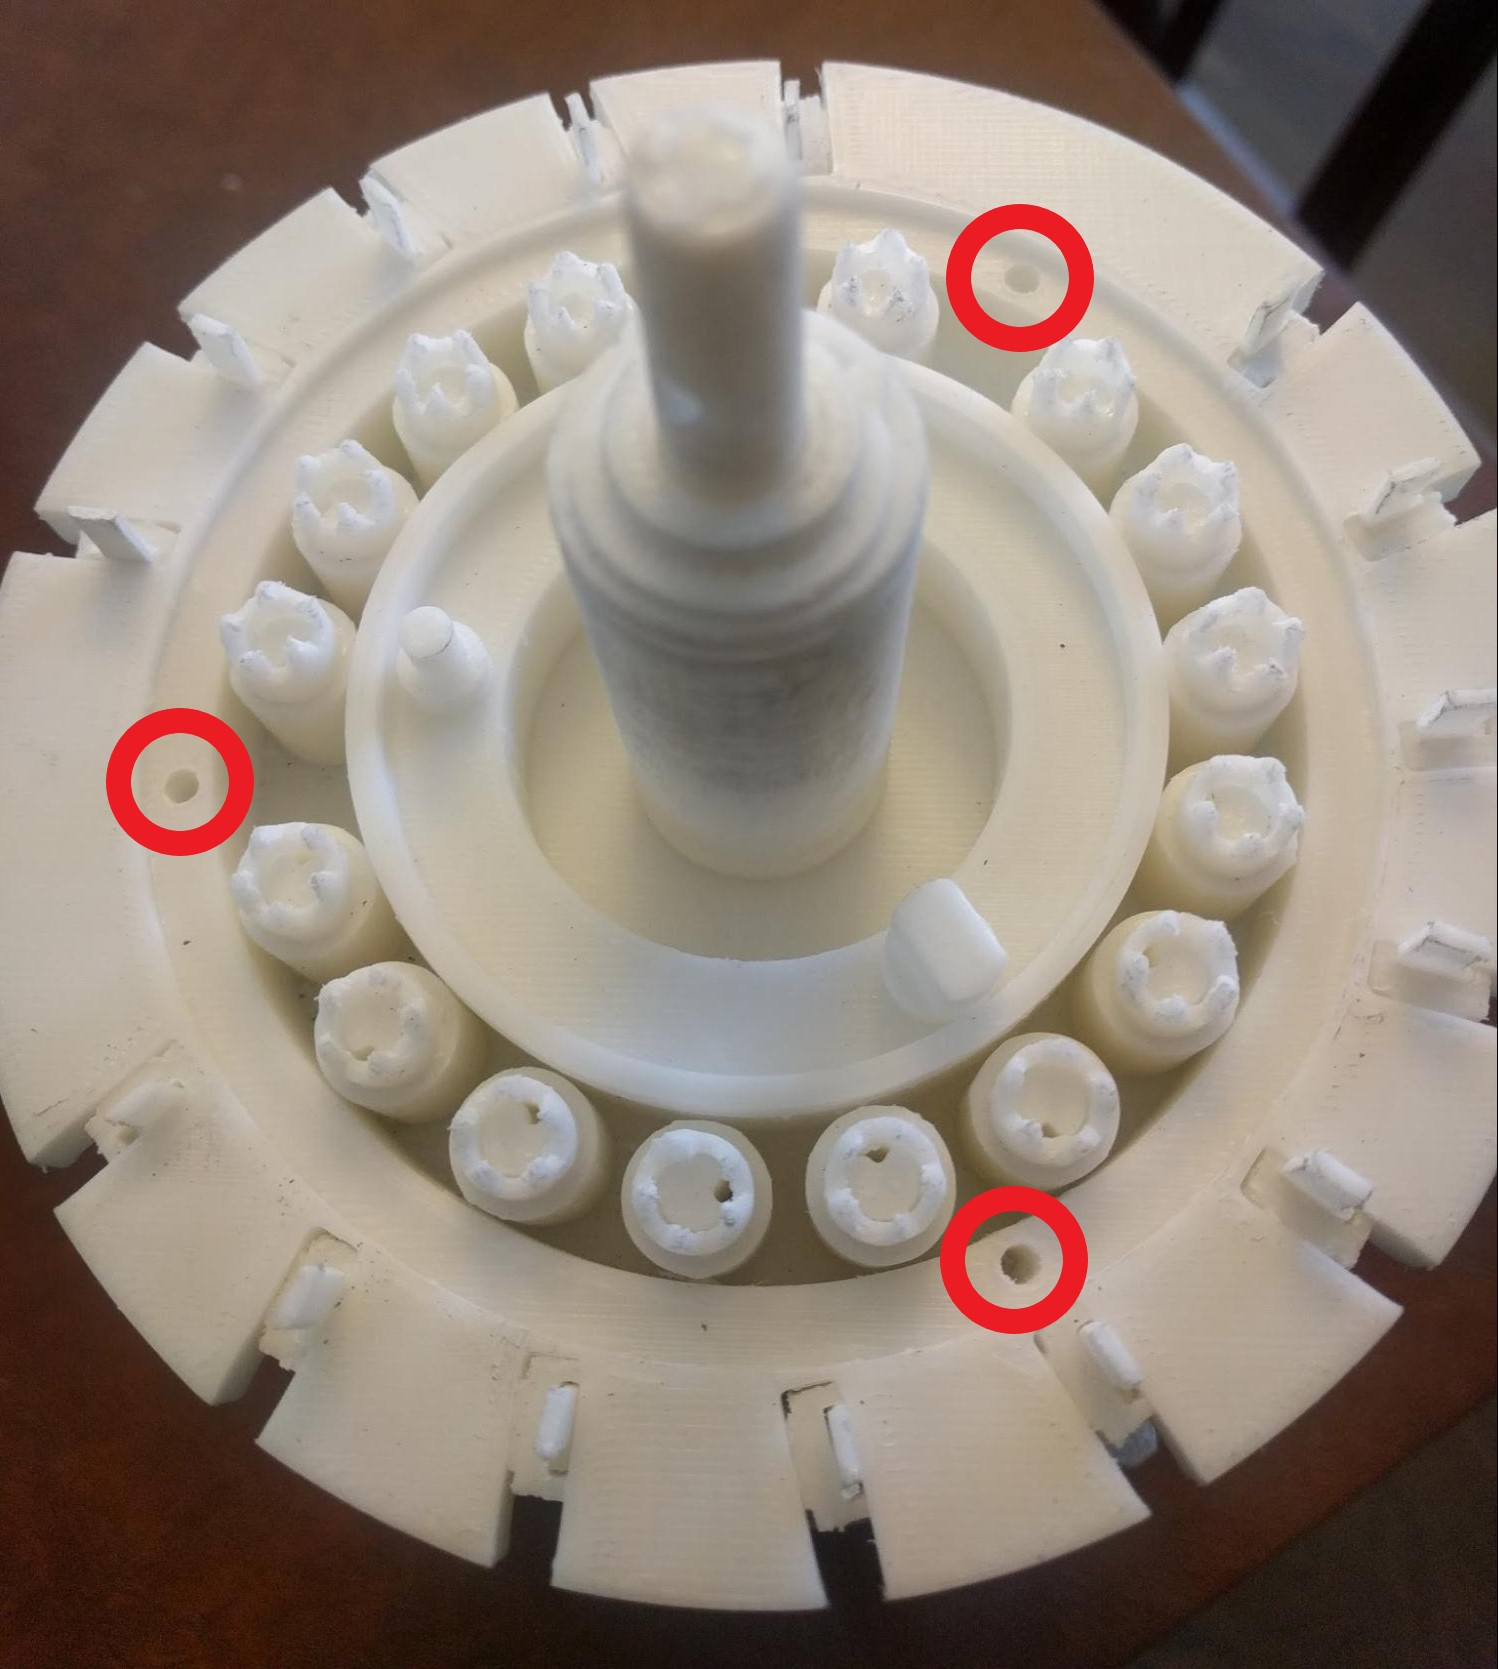
\includegraphics[width=.95\textwidth]{images/image45-circles.jpg}
		\caption{The circled holds need an M3 tap.}
		\label{fig:image45}	
	\end{subfigure}
	\begin{subfigure}{.4\textwidth}
		\centering
		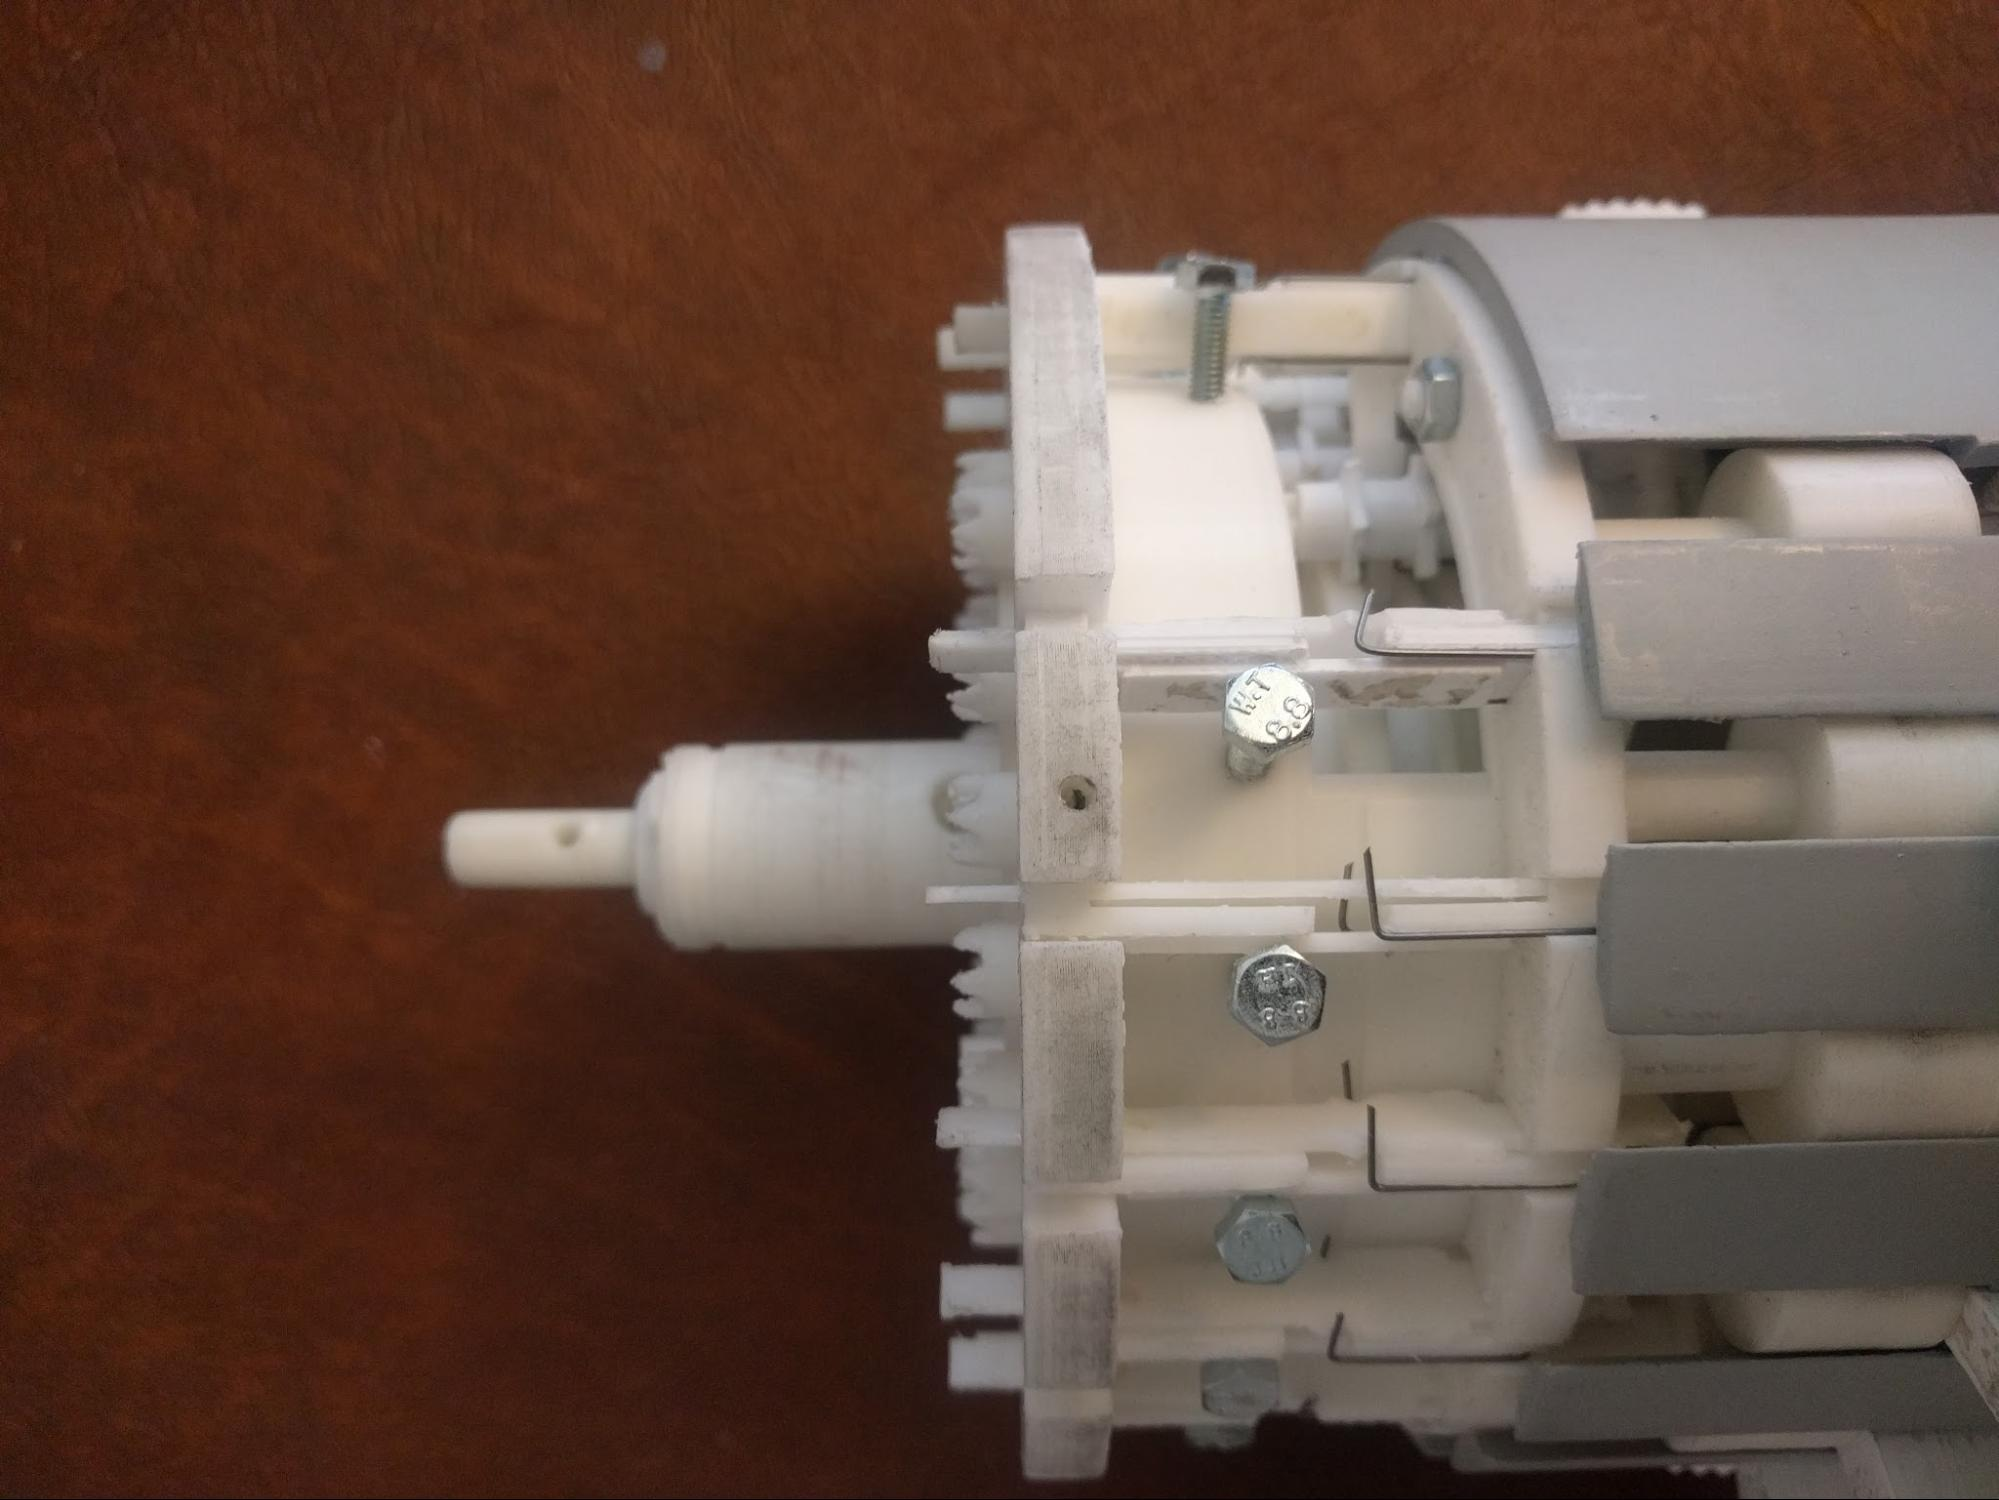
\includegraphics[width=.95\textwidth]{images/image11.jpg}
		\caption{The side holes need an M4 tap. These are pictured containing a bolt.}
		\label{fig:image11}	
	\end{subfigure}
	\caption{Tapping holes in the Main Casting}
\end{figure}

Now handle the threading necessary in the bearing plate. These are the holes to tap (refer to diagram below for locations):
\begin{itemize}
\item The holes for the selector bearing plates need an M4 tap (red in the diagram)
\item The base plate screw holes need an M5 tap (green in the diagram)
\item The hole for the anti-rotation plate screw needs an M5 tap (yellow in the diagram)
\item The anti-reversal pawl hole needs an M5 tap (purple in the diagram)
\end{itemize}

Finally, spray the holes for the transmission axles, main axle, and selector shafts on the bearing plate and the main casting with lubricant. Try to avoid the other holes in the main casting and bearing plate.


\subsection{Bearing Plate Diagram (from the bottom side)}
\begin{figure}[!ht]
	\centering
	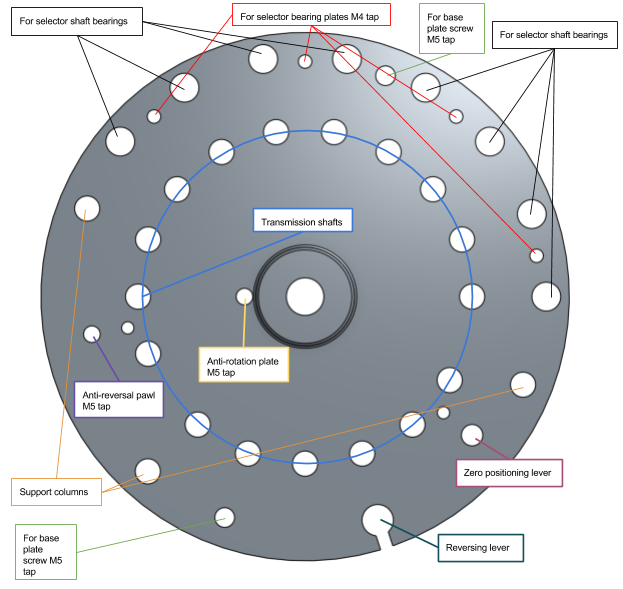
\includegraphics[width=\textwidth]{images/image25.png}
	\caption{Bearing Plate}
	\label{fig:image25}	
\end{figure}



\chapter{Step Drum and Bearing Plate}

\section{Parts Required}

\begin{table}[!ht]
 \centering
 \begin{tabular}{clc}
    Part Number & Part Name & Quantity (if $>1$) \\ \hline
     13 & Step Drum Lower or Step Drum (with main axle) & \\
     45 & Step Drum Upper Or Main Axle Bottom & \\
     49 & Anti-Rotation plate (called Anti-Reversal in BoM) & \\
     57 & Bearing Plate & \\
     78 & Step Drum Pins & 3 
   %  33 & Tens Bell & 
 \end{tabular}
\end{table}

\section{Tools Required}
\begin{itemize}
	\item Hexdriver or screwdriver (Depending on the type of bolts you have)
	\item PTFE spray lubricant
	\item Files
	\item Sandpaper
\end{itemize}

\begin{itemize}
 \item Hex driver or screwdriver (depending on the type of bolts you have)
 \item PTFE spray lubricant
 \item Files
 \item Sandpaper
 \item Superglue (cyanoacrylic)
\end{itemize}




\section{Process}
If you opted for printing the step drum as one piece, fit the main axle bottom into the base of the
step drum. This should be a snug fit with the keys matching up inside the step drum preventing any
rotation of the bottom of the axle relative to the step drum.


%\begin{wrapfigure}{r}{.45\textwidth}
\begin{figure}[!ht]
 \centering
 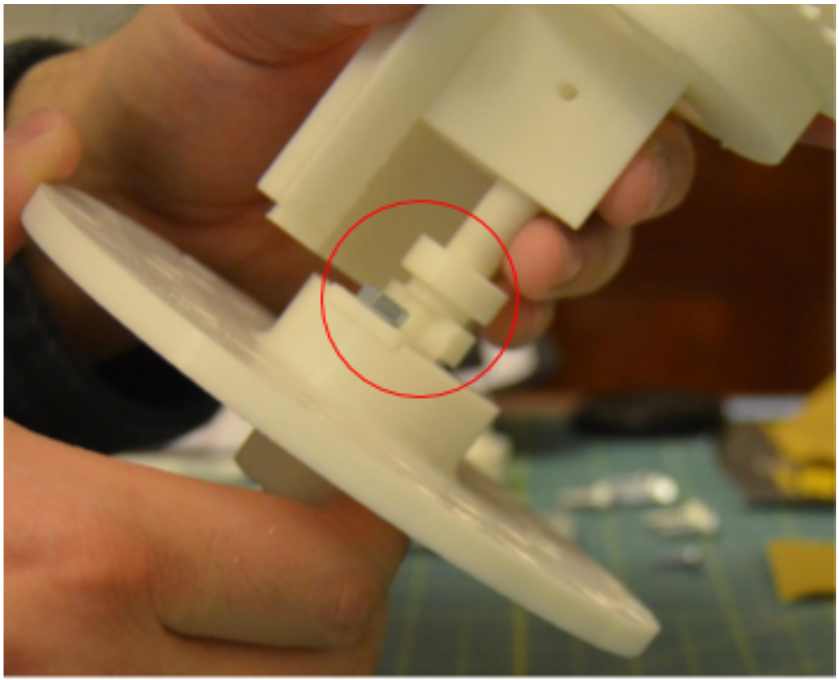
\includegraphics[width=.5\textwidth]{images/anti-rotation-collar.png}
 \caption{Alignment of the anti-rotation collar to the step drum}
\end{figure}
%\end{wrapfigure}

If you opted for printing the step drum in two pieces, fit the three pins into the lower piece of 
the step drum and super them into place. Once that has dried, add super glue to the pins of the lower
step drum and pres the upper half of the step drum onto the pins to combine the upper and lower
portions of the step drum into one piece.




The flat portion of the anti-rotation collar on the base of the axle needs to align with the right
side of the step drum when the toothed face of the step drum is facing you. This ensures that
the Curta will not switch between addition and subtraction when it is mid-rotation.



Now slide the step drum into the center of the bearing plate. The step drum should spin smoothly.
If it does not, file and sand it down until it does. Use some PTFE spray lubricant on the shaft and
the bearing plate. Do not allow the lubricant to reach the teeth of the step drum, but do allow it
to cover the anti-rotation collar. The fit should allow the step drum to spin freely. If you have to
sand further after spraying the lubricant, you will need to respray the parts that have already been
sanded.

\begin{figure}[!ht]
	\centering
	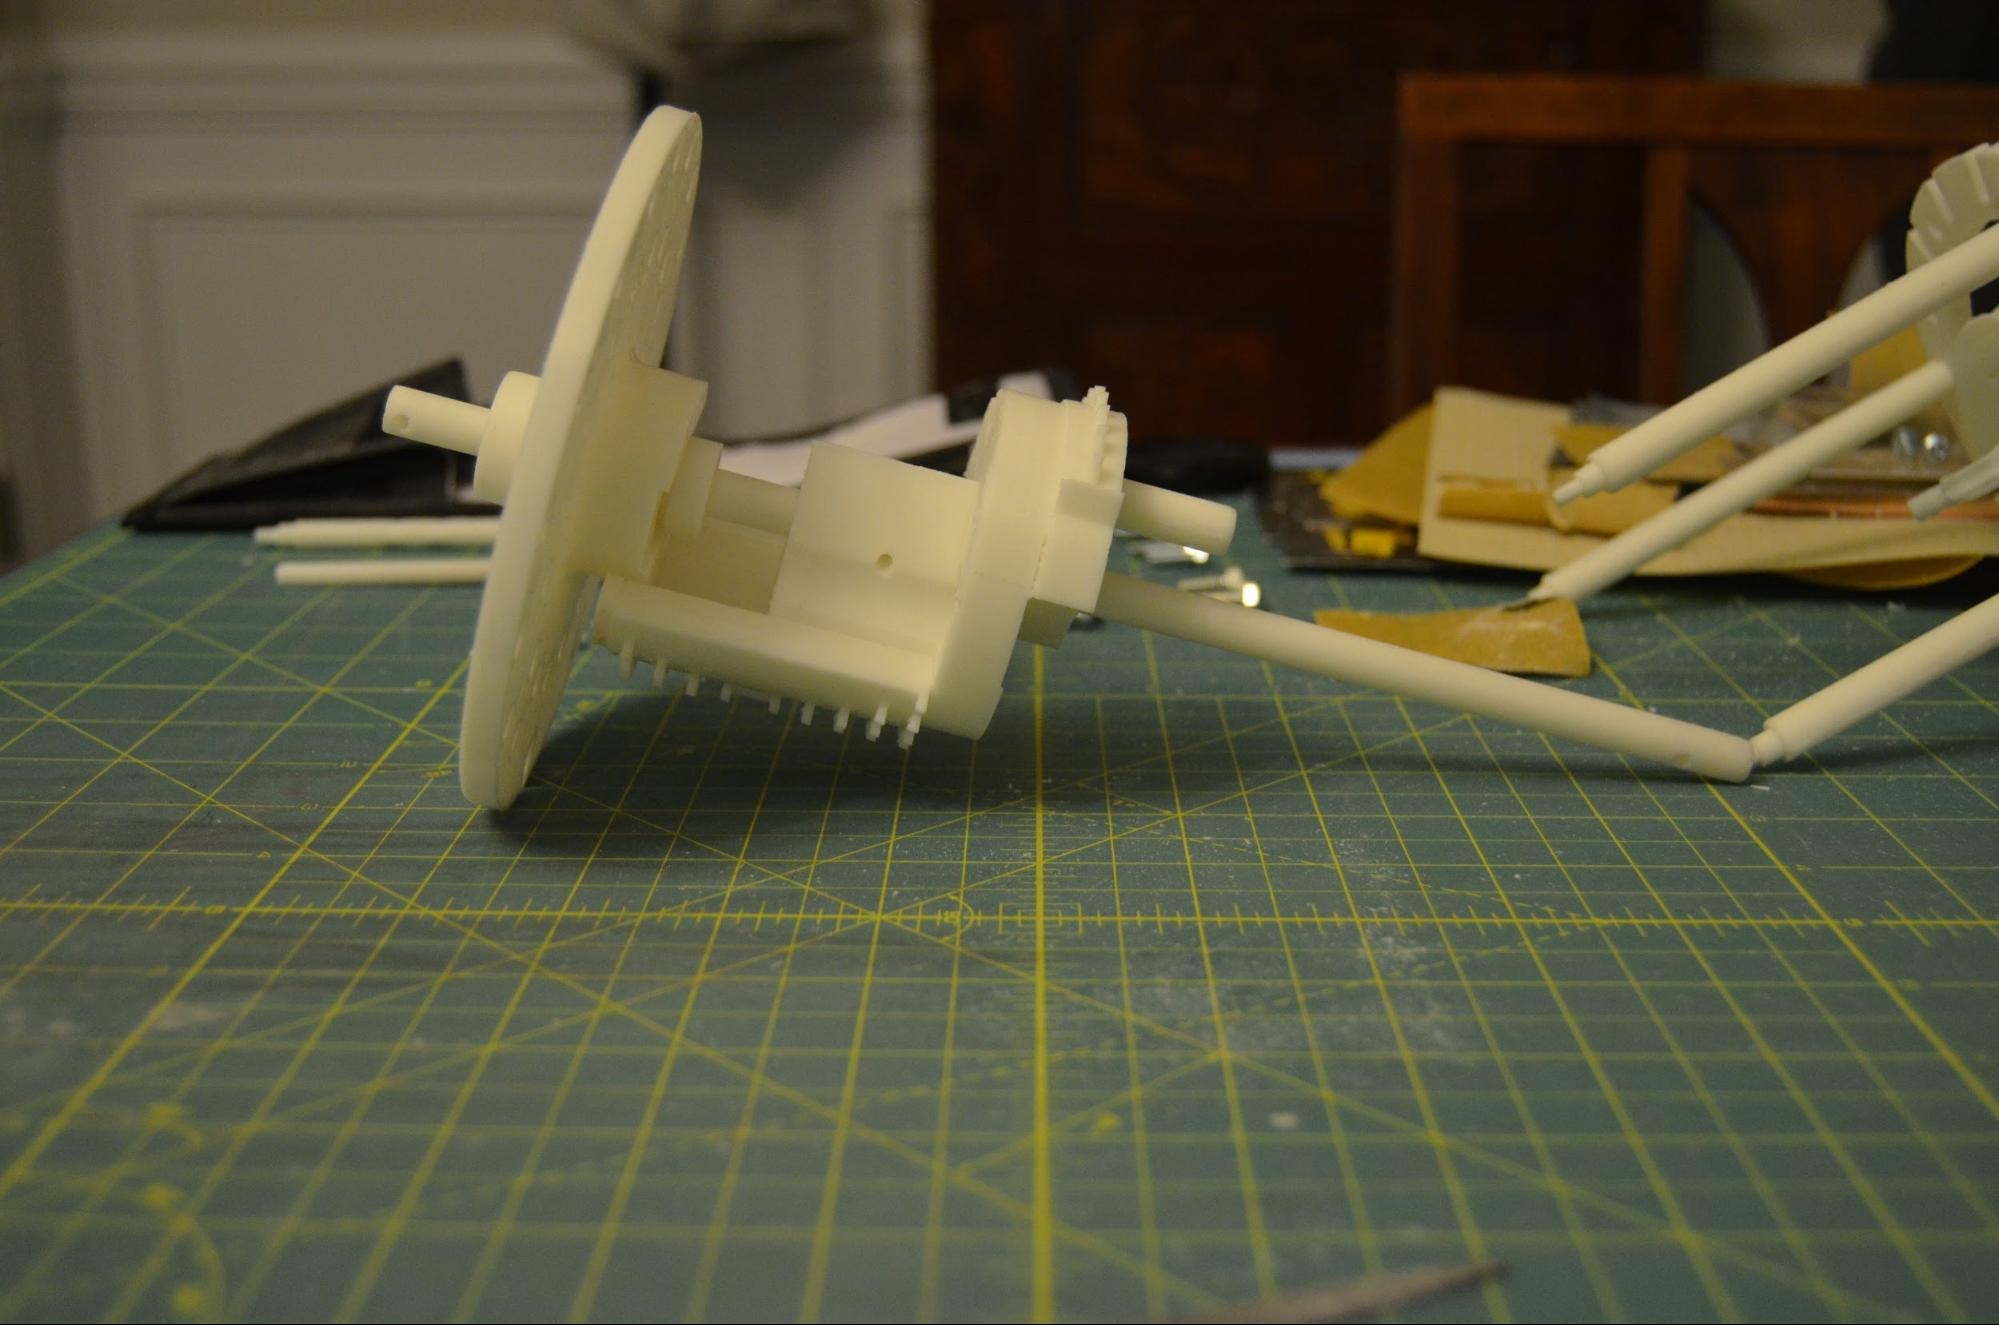
\includegraphics[width=.75\textwidth]{images/image9.jpg}
	\caption{Step Drum connected to the Bearing Plate}
	\label{fig:image9}	
\end{figure}


Place the anti-rotation plate on the recessed portion of the bearing plate near the center. Turn the
step drum until the anti-rotation plate aligns with the collar and then slide the anti-rotation
plate to meet the flat portion of the anti-rotation collar. Test this fit to check that the plate
fits in the slots in the collar and that the step drum still moves freely. Sand and file as necessary
to make that happen. The step drum may need to slide up or down to align the plate with the middle 
section of the collar to get it in the correct position.

Now use a 10mm M5 bolt to secure the anti-rotation plate ensuring that it stays press against the
ant-rotation collar. If you need to, you can put a driver through the hole at the top of the step
drum to reach the bolt. I used plier for this since I had a hex bolt. \textbf{Do not over tighten
any of the screws or nuts in this build. If you strip the plastic the part will need to be reprinted}.
Fasteners should be tight, but don't crank down too much. If it will not stay as secure as you need,
use removeable threadlock.

\begin{figure}[!ht]
	\centering
	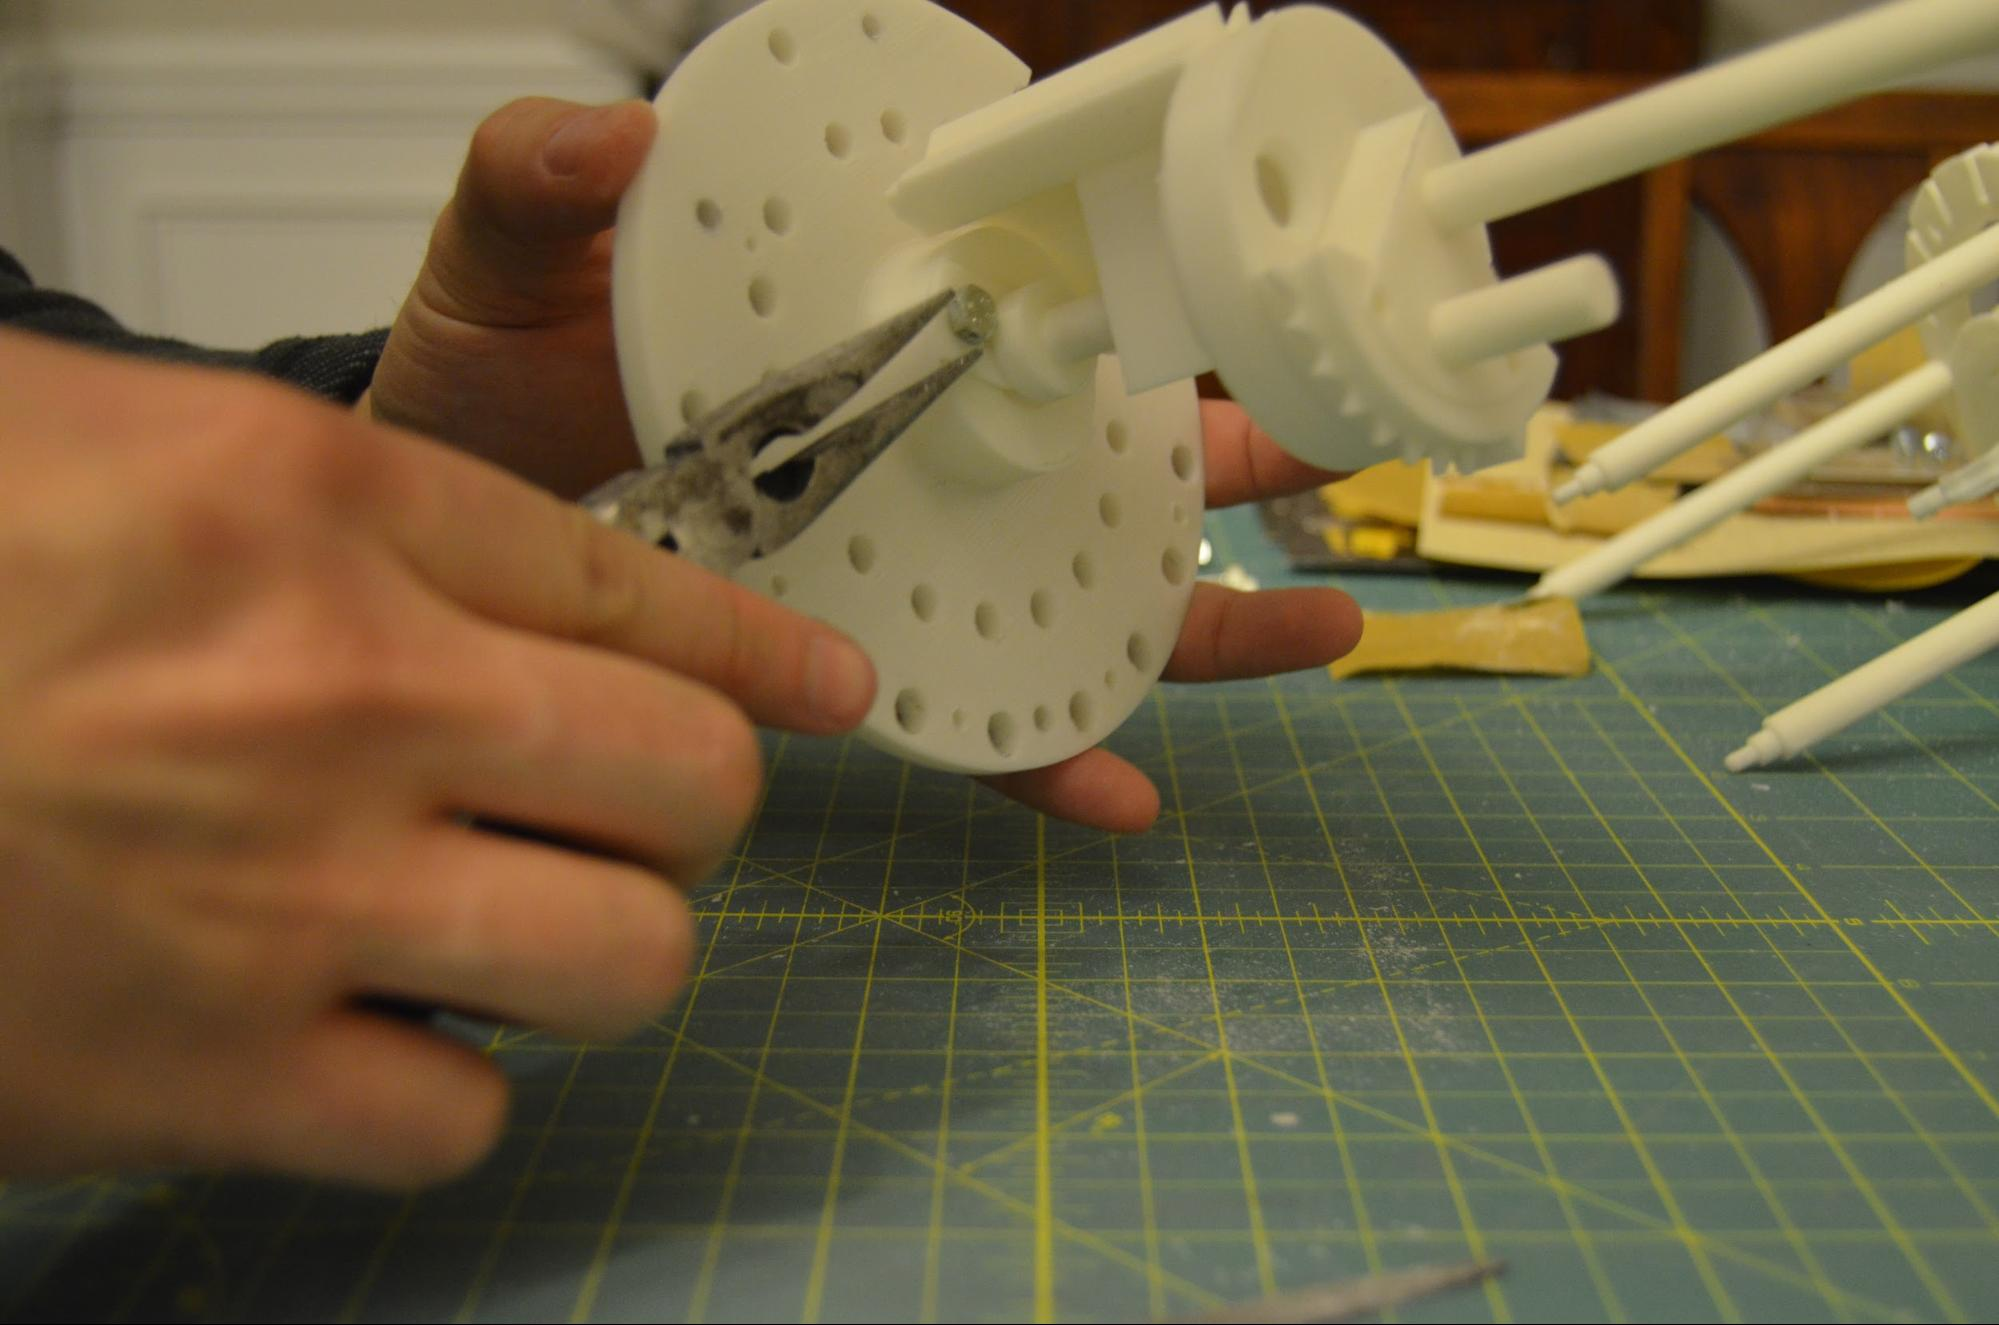
\includegraphics[width=.75\textwidth]{images/image28.jpg}
	\caption{Securing the anti-rotation plate.}
	\label{fig:image28}	
\end{figure}

Finally, double-check that you can still rotate the step drum smoothly and that the step drum can
switch between the raised (subtraction) position and the lowered (addition) position easily. If not,
you may need to file the anti-rotation plate or the collar some more and re-lubricate.



%

\chapter{Tens Bell and Main Casting}

\section{Parts Required}
\begin{table}[!ht]
	\centering
	\begin{tabular}{clc}
		Part Number & Part Name & Quantity (if $>1$) \\ \hline
		26 & Support Columns (Frame Support in BoM) & 3 \\
		33 & Tens Bell & \\
		39 & Tens Bell c-clip & \\
		40 & Tens Bell spring & \\
		48 & Retaining ring for Tens Bell & \\
		56 & Main Casting (main body in BoM) & 
	\end{tabular}
\end{table}


\section{Tools Required}
\begin{itemize}
	\item M4 threading die
	\item M4 tap
	\item Screwdriver
	\item Pliers or 4mm open ended wrench
\end{itemize}

\section{Process}

The tens bell needs to be fitted to the main casting and to the main axle. The main axle only slides up and down in the tens bell and that should move easily, but may have some friction. Some friction here is actually desired to reduce the amount of strength required in the tens bell spring.

The fit of the tens bell in the main casting should spin freely. Once the fit is right, spray the outside and inside of the sleeve of the tens bell with lubricant. Avoid spraying the rings of the tens bell. The outside and inside of the sleeve of the main casting also needs lubrication. Once done, the main casting should make multiple revolutions when holding the tens bell at the bottom and spinning the main casting.

Remove the tens bell and use an M4 tap in the two small holes through the body of the tens bell, see Figure \ref{fig:image54}. Place the tens bell spring inside the tens bell body aligning it with the two threaded holes and the hole for the main shaft, Figure \ref{fig:image4}. Use two M4 screws to secure it. Try not to pry the legs of the spring too far apart with the screwdriver. Slide the tens bell back into the main casting, place the retaining ring over the tens bell so it rests on the main body, and secure the tens bell and retaining ring with the C-clip, Figure \ref{fig:image47}.

\begin{figure}[!ht]
	\centering
	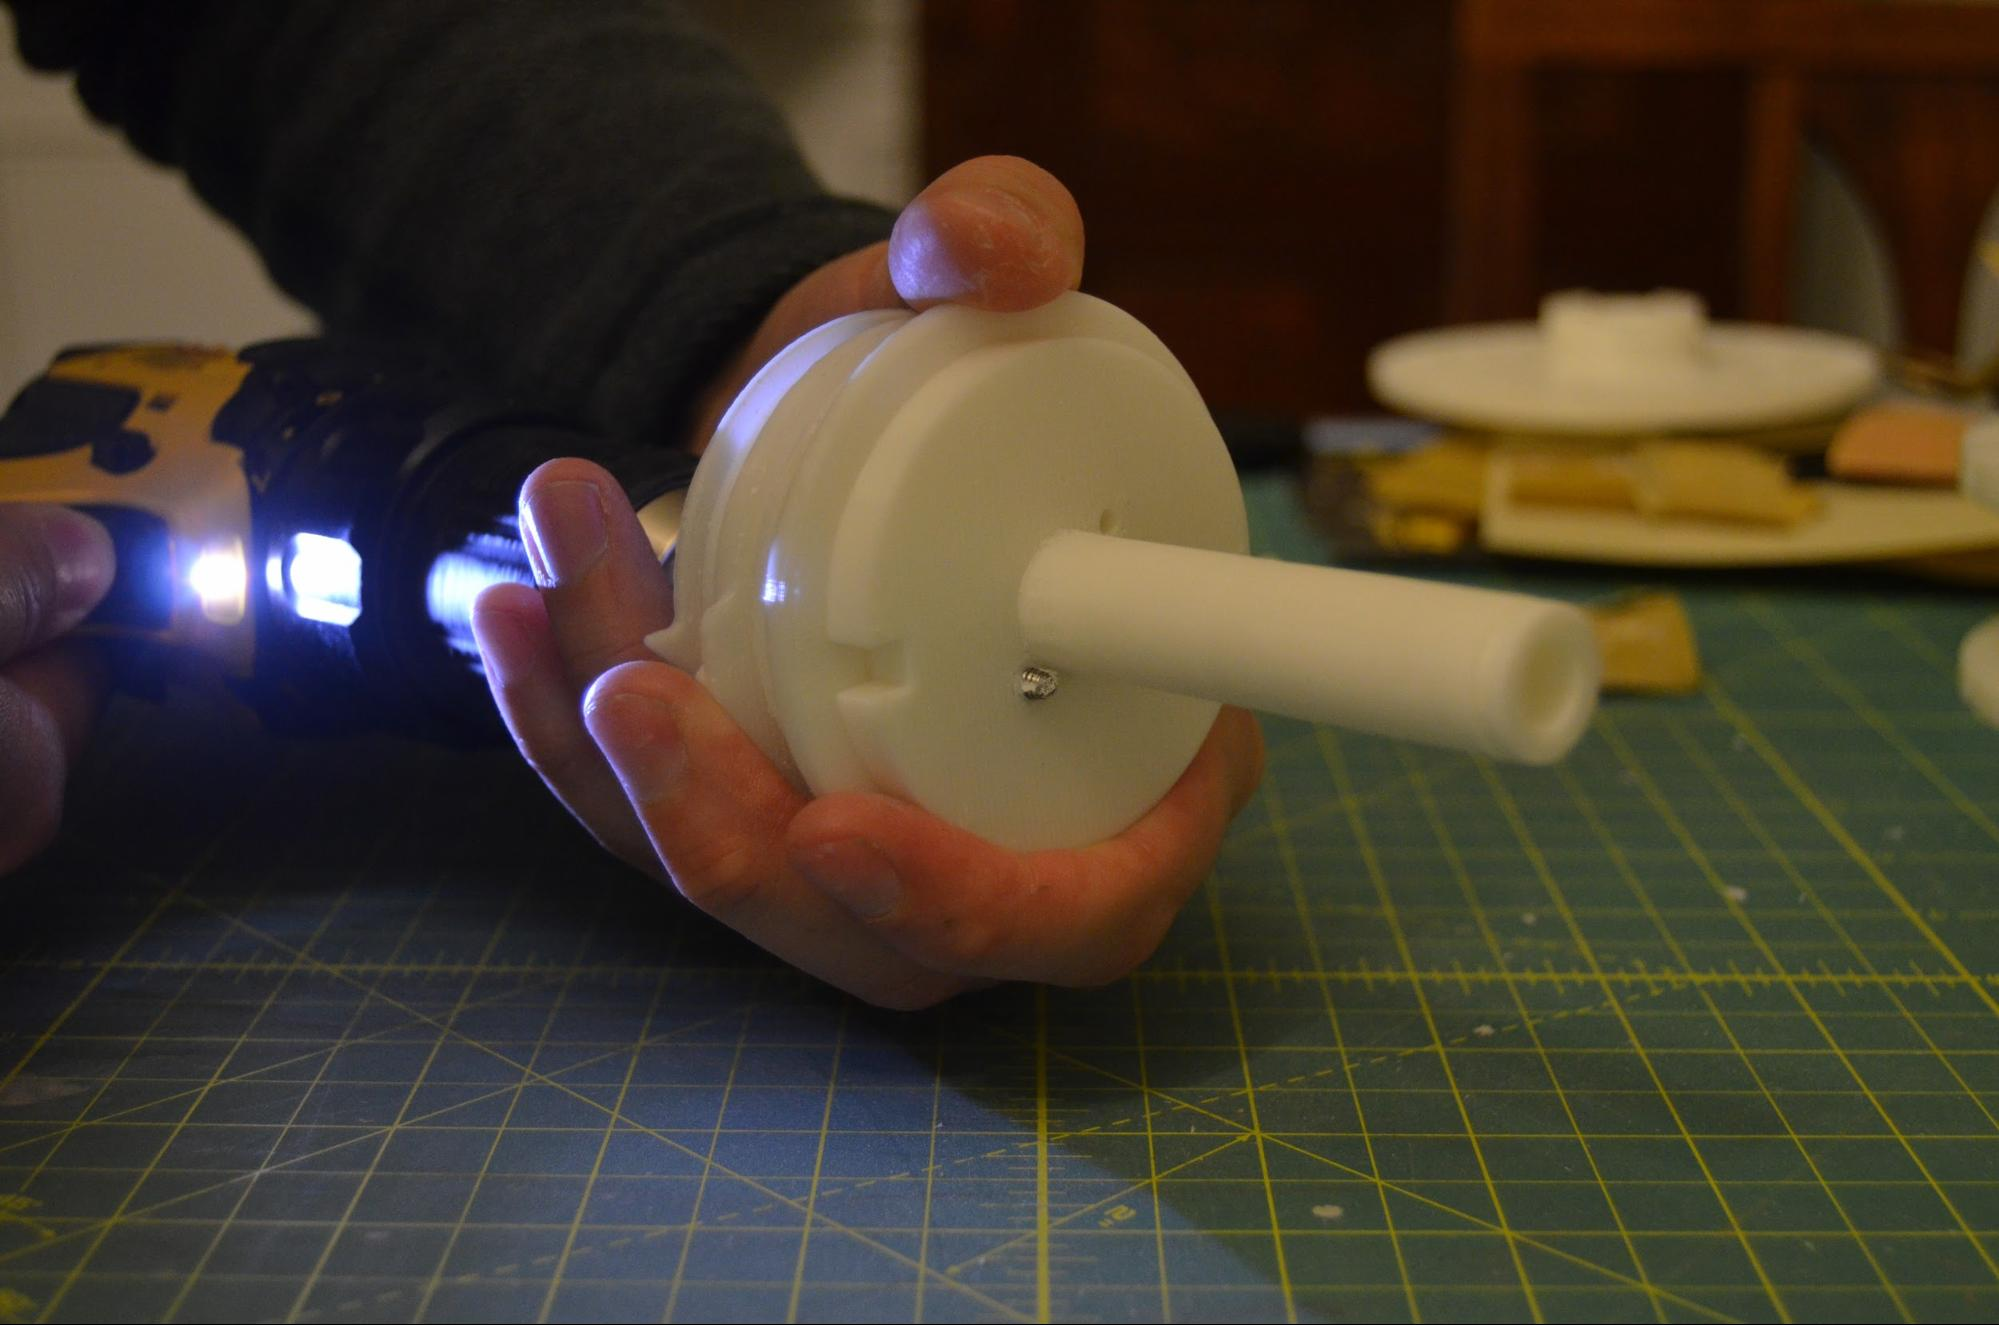
\includegraphics[width=.75\textwidth]{images/image54.jpg}
	\caption{Tapping the holes in the Tens Bell with an M4 tap.}
	\label{fig:image54}	
\end{figure}


\begin{figure}[!ht]
	\centering
	\begin{subfigure}{.4\textwidth}
		\centering
		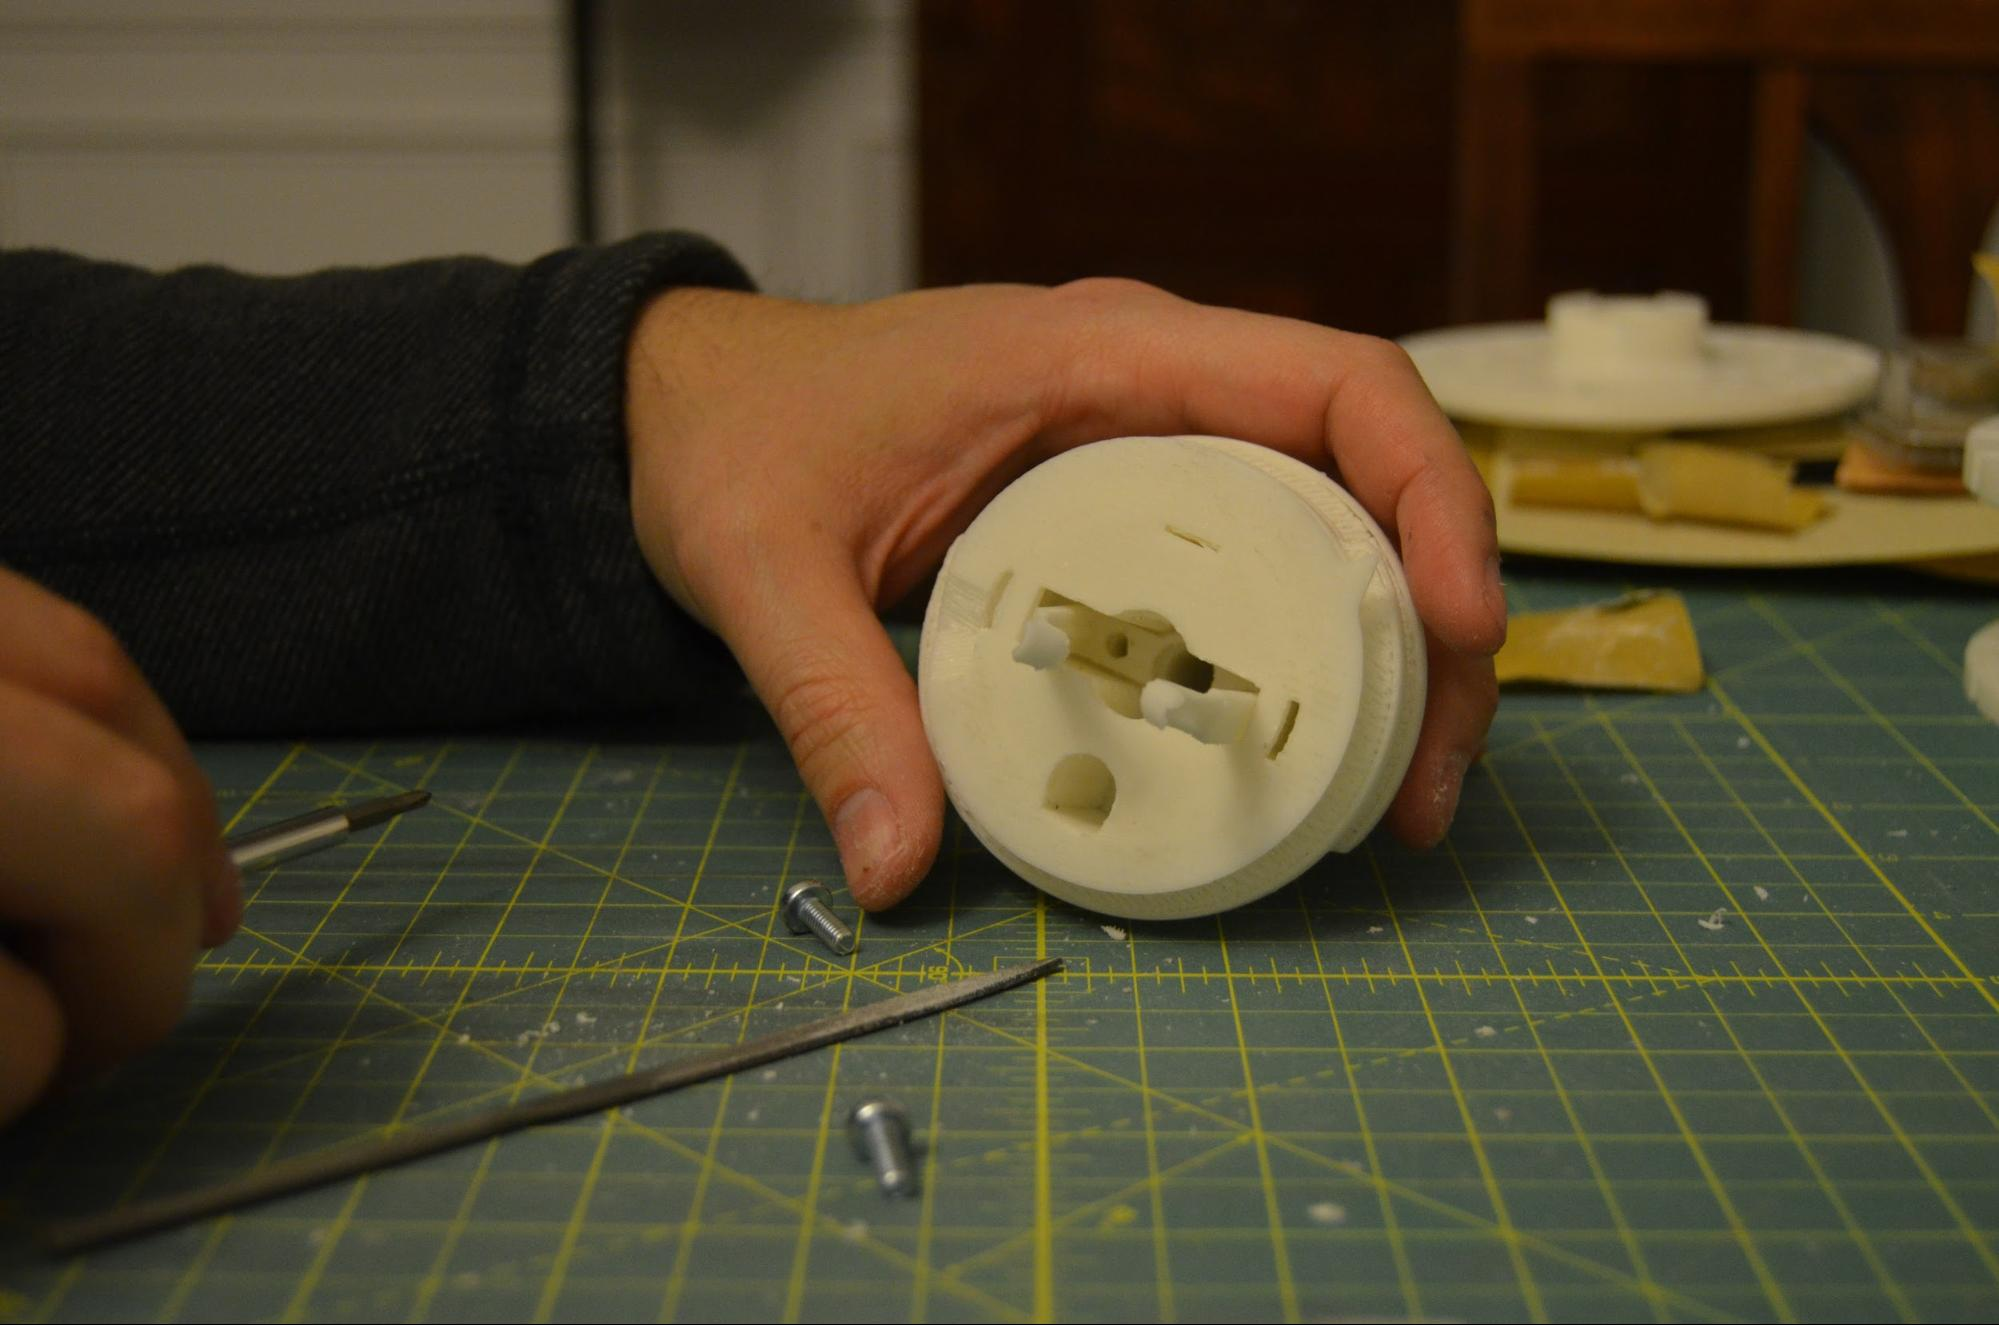
\includegraphics[width=.95\textwidth]{images/image4.jpg}
		\caption{Installing the Tens Bell Spring.}
		\label{fig:image4}	
	\end{subfigure}
	\begin{subfigure}{.4\textwidth}
		\centering
		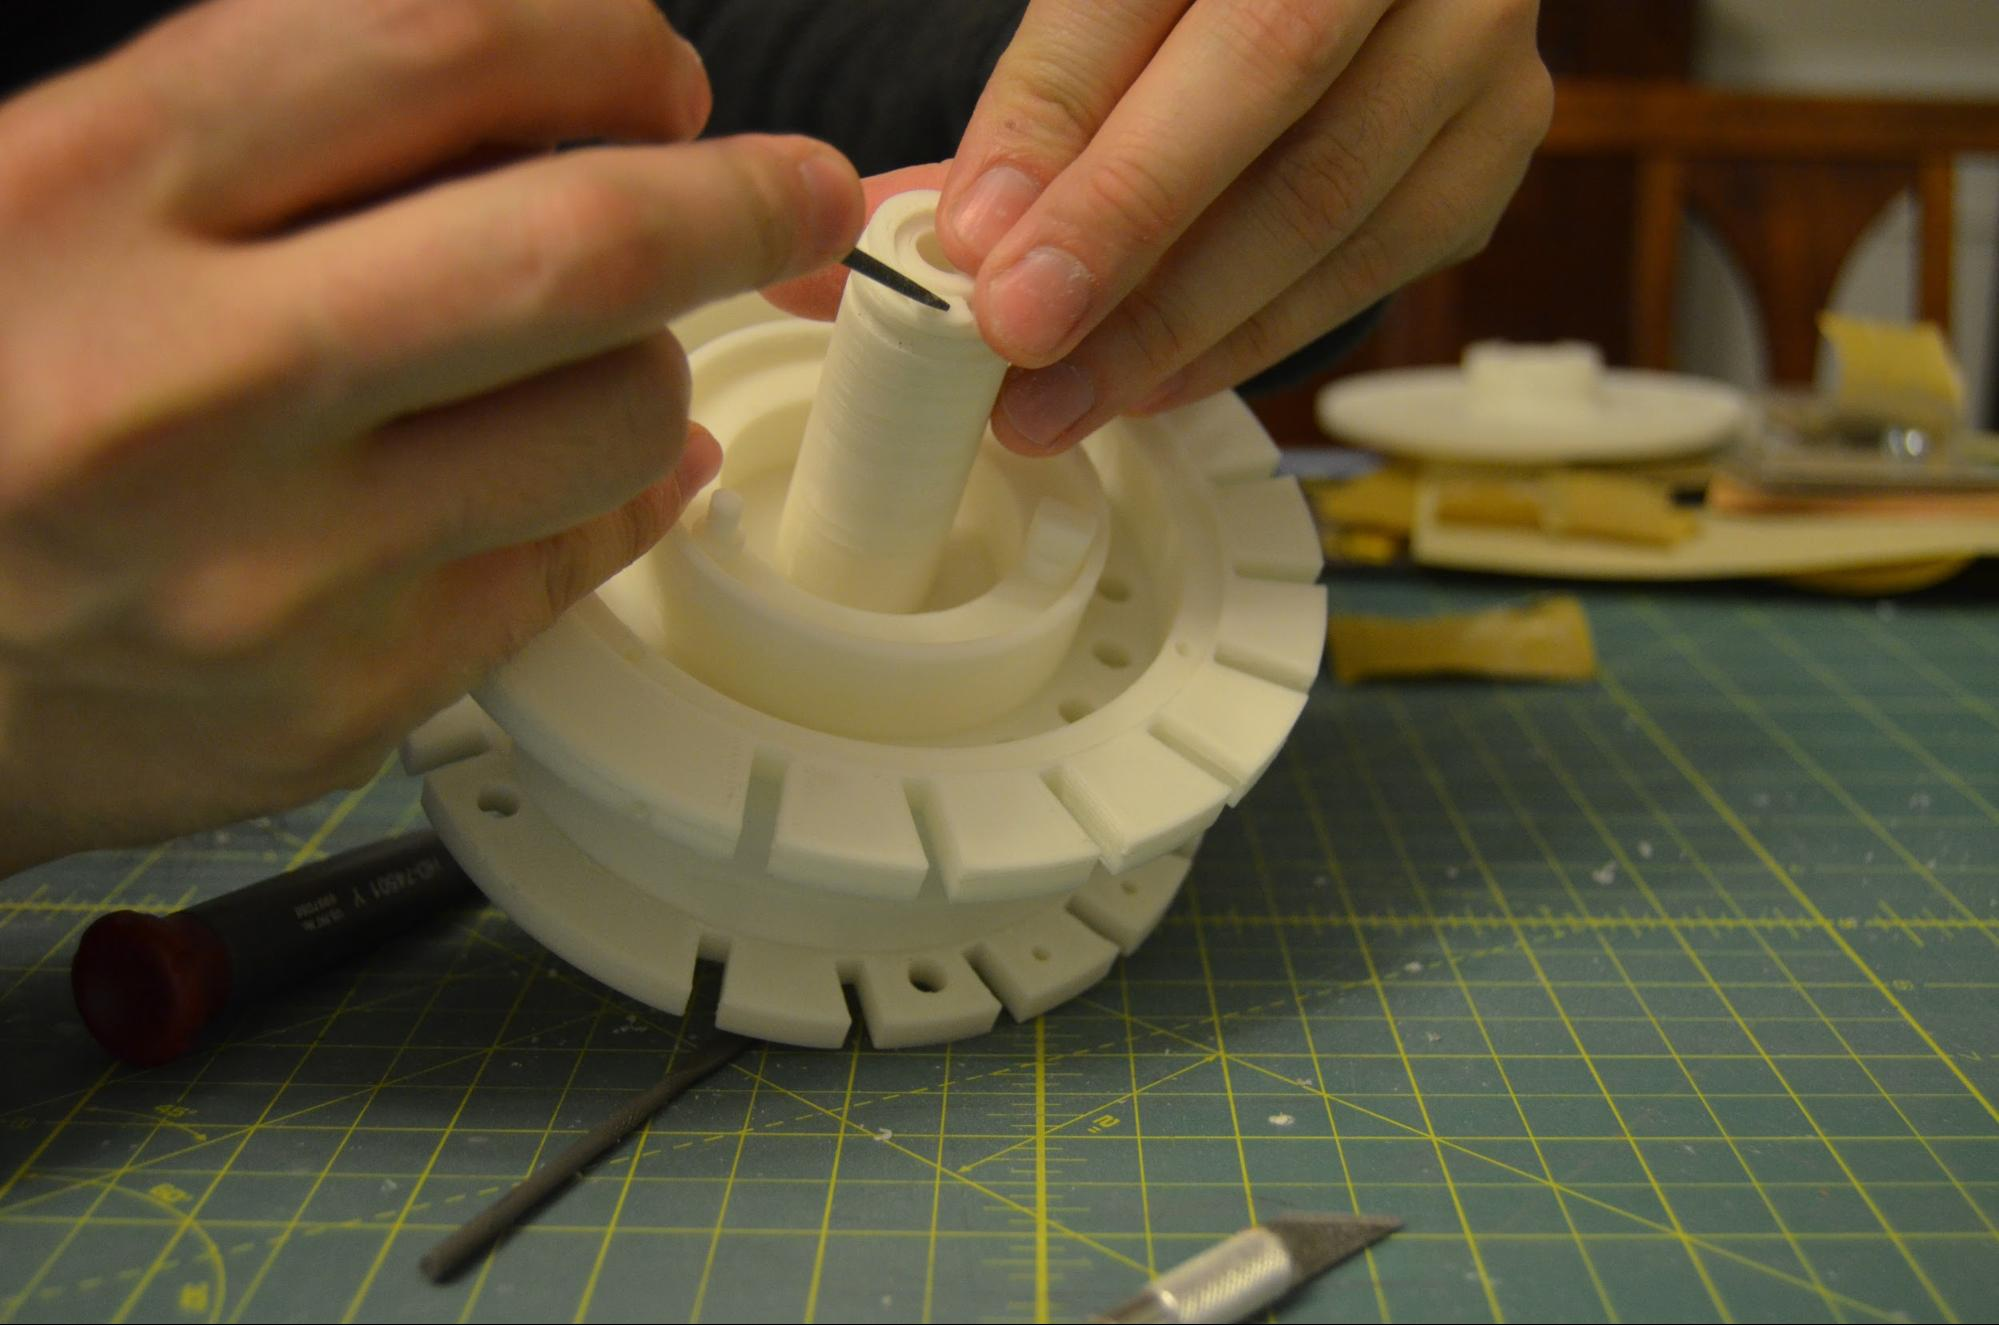
\includegraphics[width=.95\textwidth]{images/image47.jpg}
		\caption{The Tens Bell C-clip goes in the grove in the top of the Tens Bell, over the Retaining Ring.}
		\label{fig:image47}	
	\end{subfigure}
	\caption{}
\end{figure}

The support columns should have been fit earlier, but are not yet threaded. To do that, use an M4 die. The support columns have two steps down in diameter on either end. The first step down fits into the main casting and the bearing plate. The final step down is the portion that needs threading circled in Figure \ref{fig:image14}. File down that portion until the layer lines are not visible and the outer edge is not wider than the highest the threads should be.

\begin{figure}[!ht]
\begin{subfigure}{.4\textwidth}
	\centering
	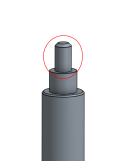
\includegraphics{images/image14.png}
	\caption{Top of the Support Columns, to be threaded with M4 die.}
	\label{fig:image14}	
\end{subfigure}
\begin{subfigure}{.5\textwidth}
	\centering
	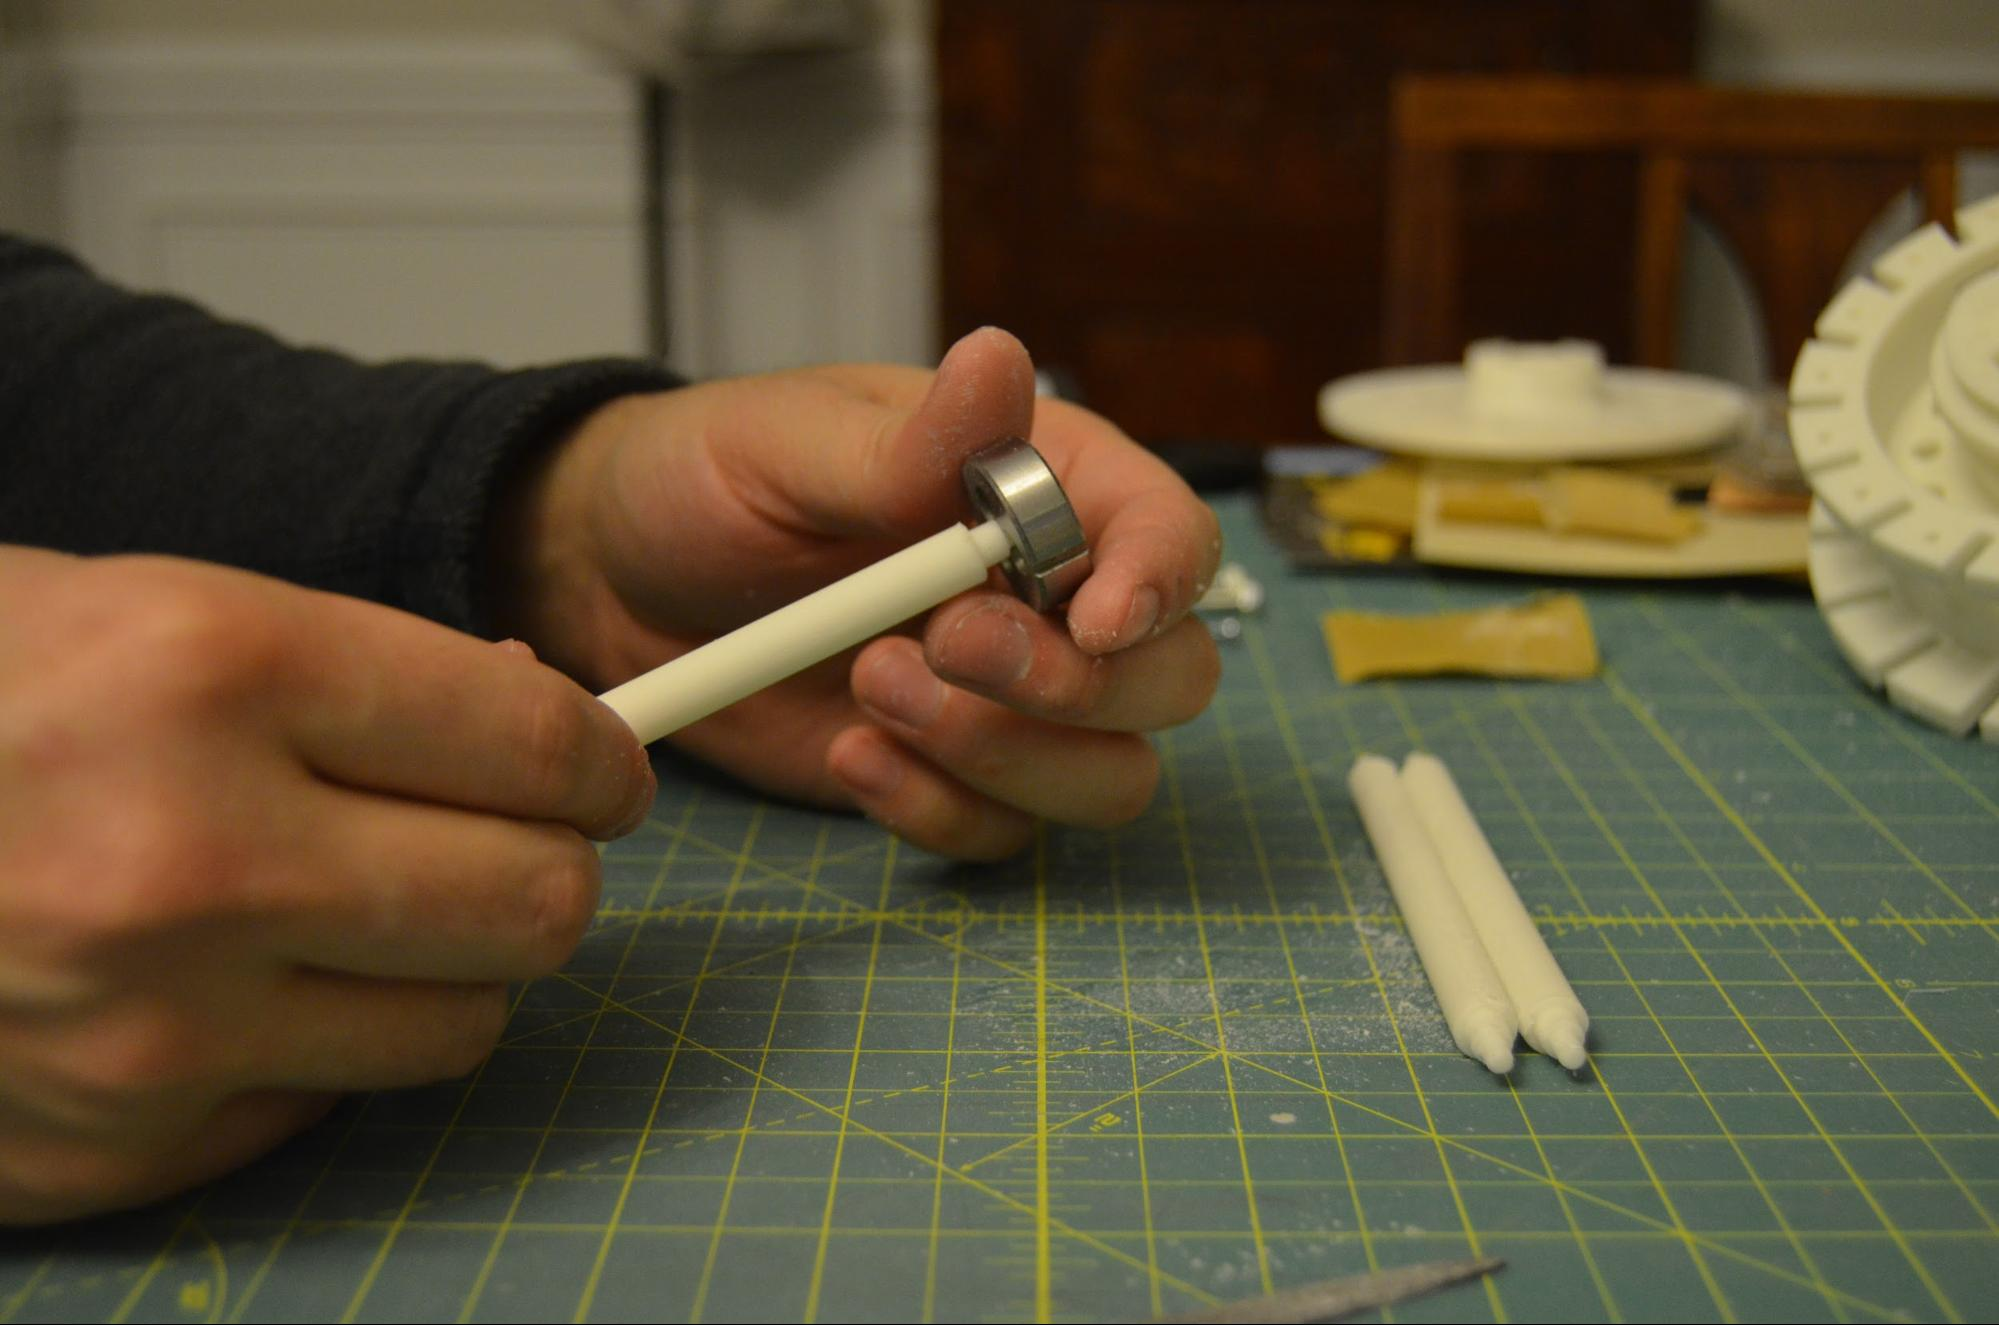
\includegraphics[width=.95\textwidth]{images/image41.jpg}
	\caption{Finish threading the Support Columns.}
	\label{fig:image41}	
\end{subfigure}
\caption{}
\end{figure}

Place the die flat on a table and the support column upright vertically. Hold it straight up while turning the dial counter-clockwise. It is much easier to keep the support column vertical if we don’t turn the column, but turn the die instead. If the column doesn’t get threaded straight, the threads can get stripped or the end can snap off while threading it. After it gets started, it will guide itself at which point the die may be picked up off the table and the column may be turned instead of the die. Every quarter turn, reverse the turn of the die to help clear out the plastic shavings and make the threading happen easier before resuming the original direction.




Once the die has been turned as far as it will go, remove the die from the part, flip the threading die over, and put the support column back through with the die backwards. This way the thread can be cut completely down that section of the support column.

Now place each of the support columns into the main casting and use an M4 nut to secure them. Use the pliers or wrench to tighten the nuts. \textbf{Do not over-tighten!} This is just plastic and those threads can strip easily. The nuts should be snug, but not a lot of force is required. This can now be set to the side for a while as work is done on other parts.

\begin{figure}[!ht]
	\centering
	\begin{subfigure}{.4\textwidth}
		\centering
		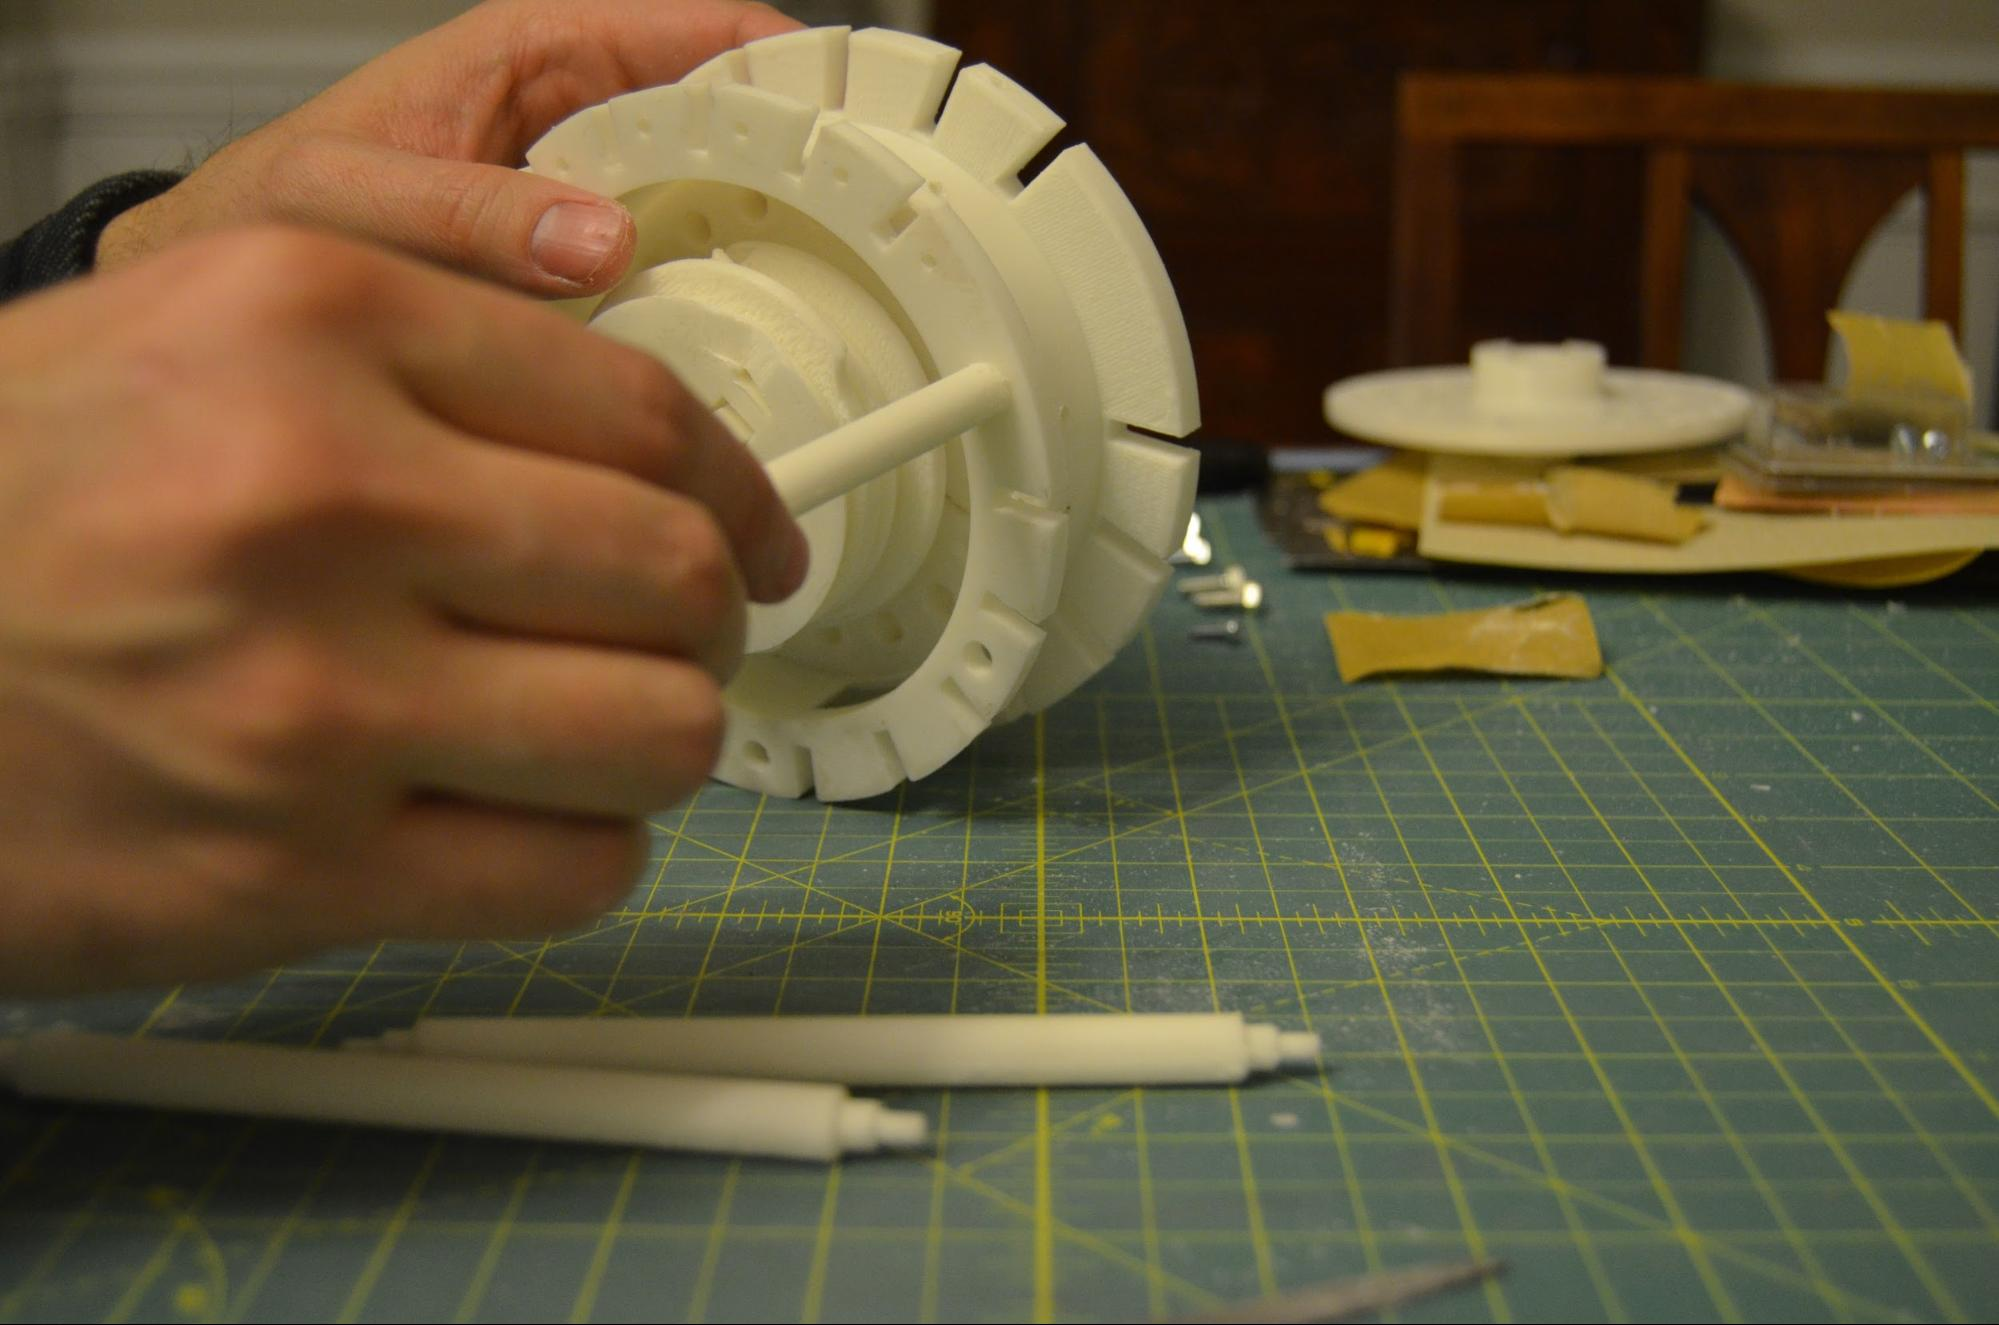
\includegraphics[width=.9\textwidth]{images/image60.jpg}
		\caption{Insert Support Columns into Main Casting.}
		\label{fig:image60}	
	\end{subfigure}
	\begin{subfigure}{.4\textwidth}
		\centering
		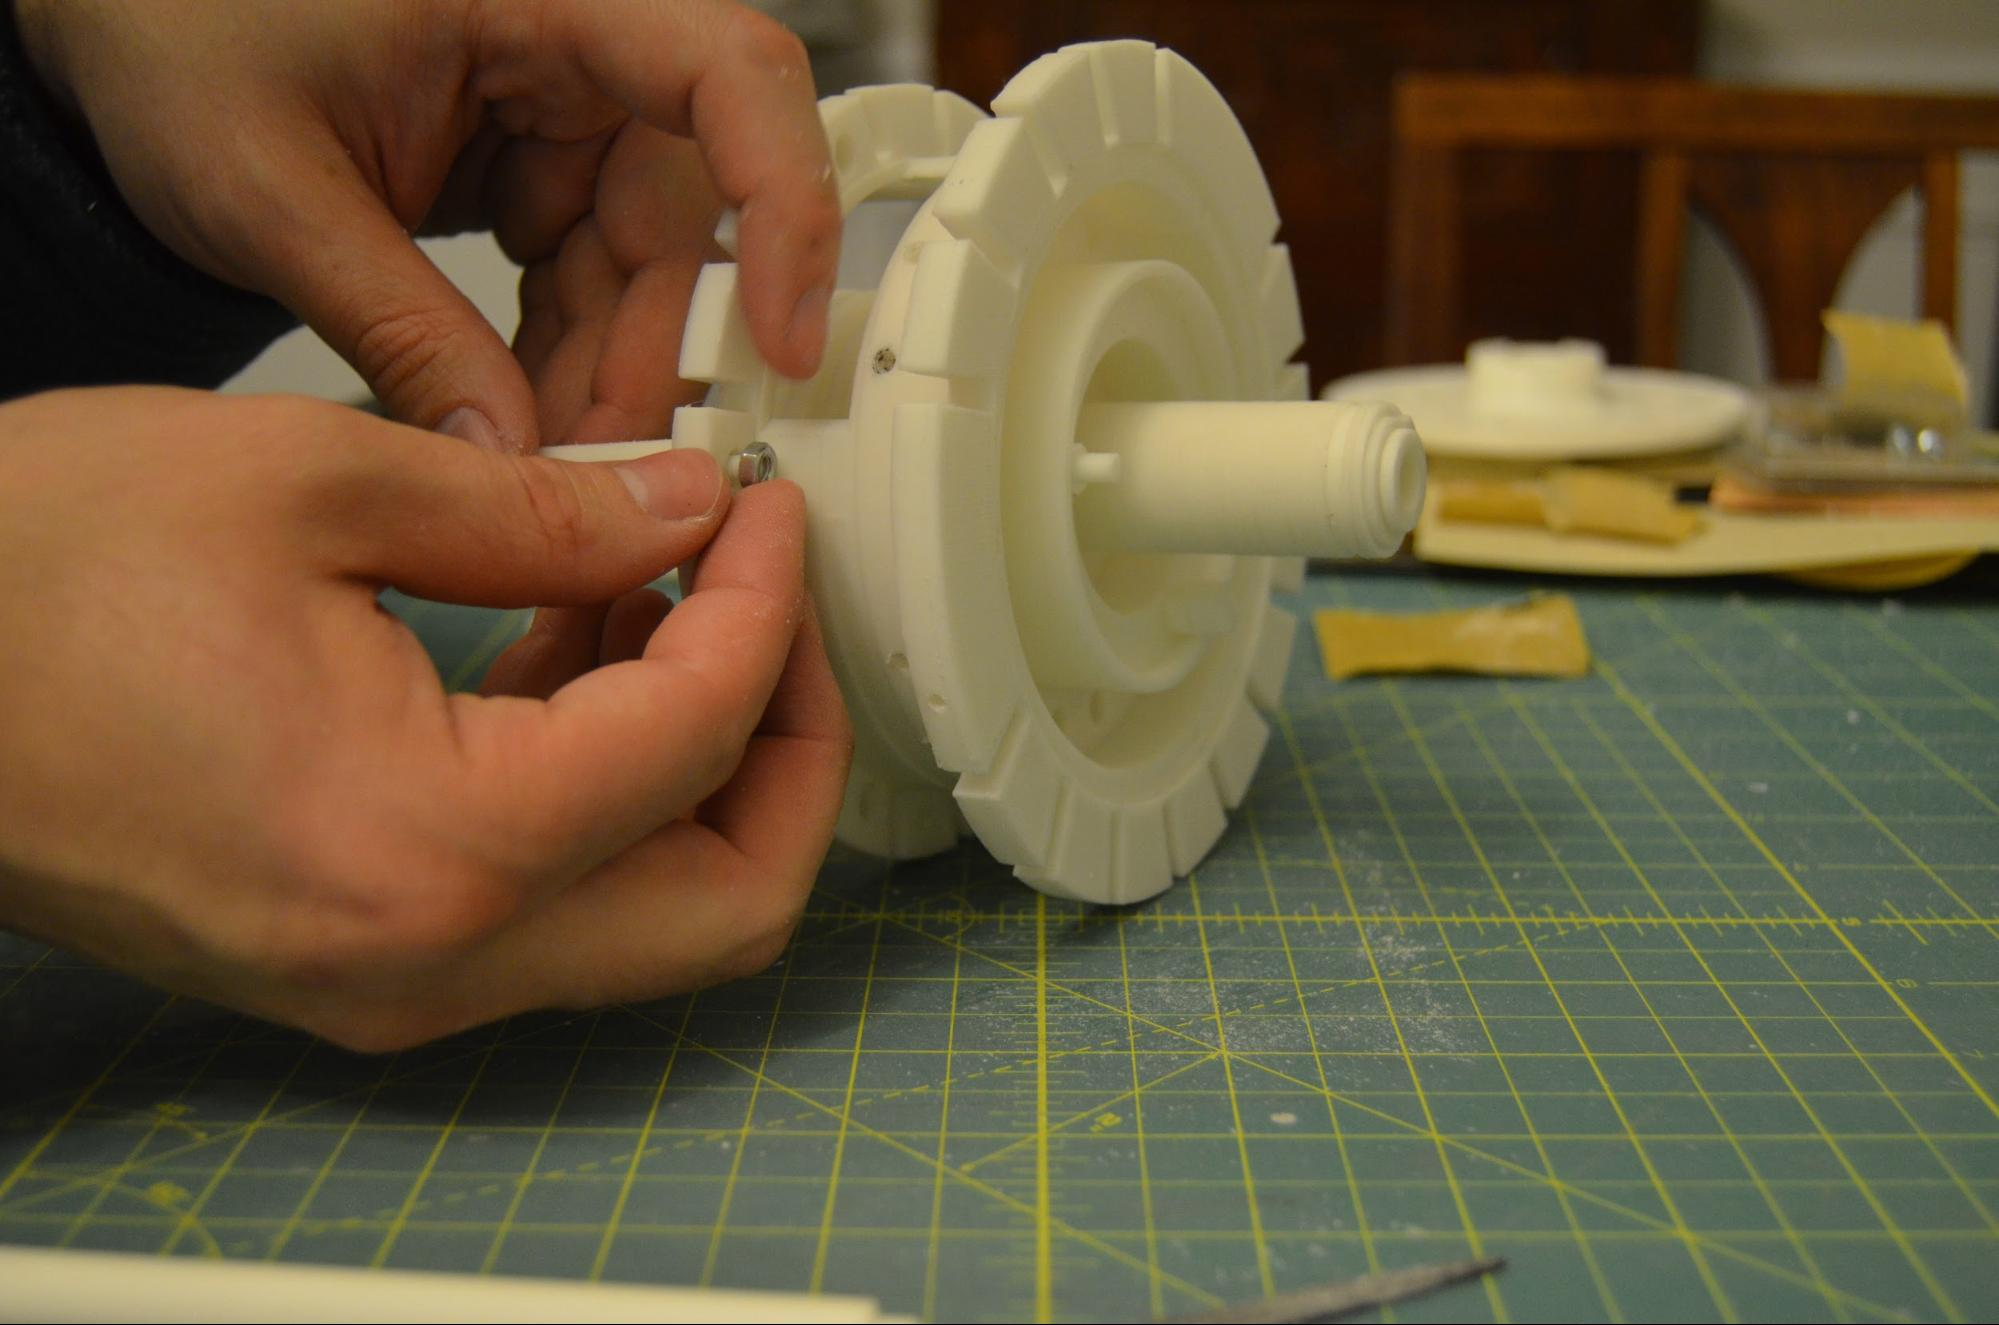
\includegraphics[width=.9\textwidth]{images/image37.jpg}
		\caption{Securing Support Columns with M4 nut.}
		\label{fig:image37}	
	\end{subfigure}
	\caption{}
\end{figure}



\chapter{Springs for Zero Positioning Lever and Anti-Reversal Pawl}
\section{Parts Required}
\begin{table}[!ht]
	\centering
	\begin{tabular}{clc}
		Part Number & Part Name & Quantity (if $>1$) \\ \hline
		17 & 0.6mm Music Wire (0.024in) & \\
		18 & 1.1mm Music Wire (0.043in) & 
	\end{tabular}
\end{table}



\section{Tools Required}
\begin{itemize}
	\item Pliers
	\item Drill
	\item Bench vice if your drill cannot stand on its own
	\item Wire Cutters
	\item $\frac{3}{8}$'' drill bit (9mm or 10mm Metric) with round shank
	\item Leather work gloves
	\item Eye protection
	\item Oven or toaster oven
\end{itemize}

\section{Process}
\textcolor{red}{WARNING:} Please use care when making these springs, the process can be dangerous if care is not taken. Serious injury could result from the wire rapidly unwinding! Wear gloves and eye protection!


Suitable springs for these two parts could not be found so they have to be made. The process is fairly simple, but care must be taken to avoid injury. This step involves working with wire at tension. Please take care to wear eye protection and hand protection.

The basic process is to chuck the music wire and drill bit into your drill and use the drill’s shank to turn torsion springs. Start with the 0.6mm wire. If you are using a 9mm drill bit, you may need to wrap some painter’s tape around it to make it larger (to about 9.5mm). Make sure that the music wire is held securely by the chuck of the drill and runs along the drill bit. Bend the wire 90 degrees away from the drill bit. Rotate the drill chuck to put the wire trailing off to the left of the drill. These are left-hand wound springs, but they wind the opposite direction that the drill turns so set the drill for clockwise / forward rotation.

Wearing your safety goggles and work gloves, grab the wire near the drill bit with your left hand. With your right hand, \textbf{slowly} run the drill while putting tension on the wire with your left hand to keep the wraps tight and the trailing wire slightly behind the current wrap. As it rotates, the current wrap will have a little gap between it and the previous wrap, but as wrapping continues the next wrap will press it against the previous.

The first spring needs seven wraps, but turn a few more wraps than you need. Once you have your spring turned, reverse the drill’s turning direction and run it slowly to release the tension on the wire. Once the tension is released, unchuck the drill bit and spring. Clip the spring off of the wire in the box of music wire leaving a little extra as a leg. The inside diameter should measure about 15mm. A millimeter or so more is ok, but smaller than 15mm will be a problem.

The second spring uses the 1.1mm diameter wire. It needs to have a 15.6mm inner diameter, but the thicker wire will not rebound as much so we need a larger arbor. To do this, tightly wrap the shank of the drill with painter’s tape until it is about 11.5mm in diameter. An 11mm drill bit may be able to be used, but I haven’t tried. With the tape-wrapped drill bit, proceed with the same process as before, but this time you don’t need as many turns of the wire. When the bit and wire are chucked into the drill, it may not chuck as tightly since the tape will compress some. Be sure that the wire is secure! This second spring requires five wraps, but as before, turn a few more than you need.

Once both springs have been turned, place them in an oven at $450^\circ$F ($232^\circ$C) for 30 minutes. A small toaster oven will suffice. Be careful here and make sure to keep an eye on it. A little bit of oil on the wire could cause a fire. Allow the springs to cool slowly / naturally inside the oven. 

Once the wires are cool, cut the wires to length. With the spring utilizing the smaller wire diameter, place one leg of the spring to your left and count seven wraps upwards. Insert your pliers 90 degrees from when it would complete the 8th wrap and bend the wire 90 degrees at that point to create the second leg. Extra coil may need to be straightened. Clip off extra leaving about $\frac{3}{4}$" or about two centimeters on each leg.

On the spring made from the larger diameter wire, insert the pliers 50 degrees from when it would complete the 6th wrap and bend the wire 90 degrees to create the second leg. Again, extra coil may need to be straightened and extra should be clipped off.

\begin{figure}[!ht]
	\centering
	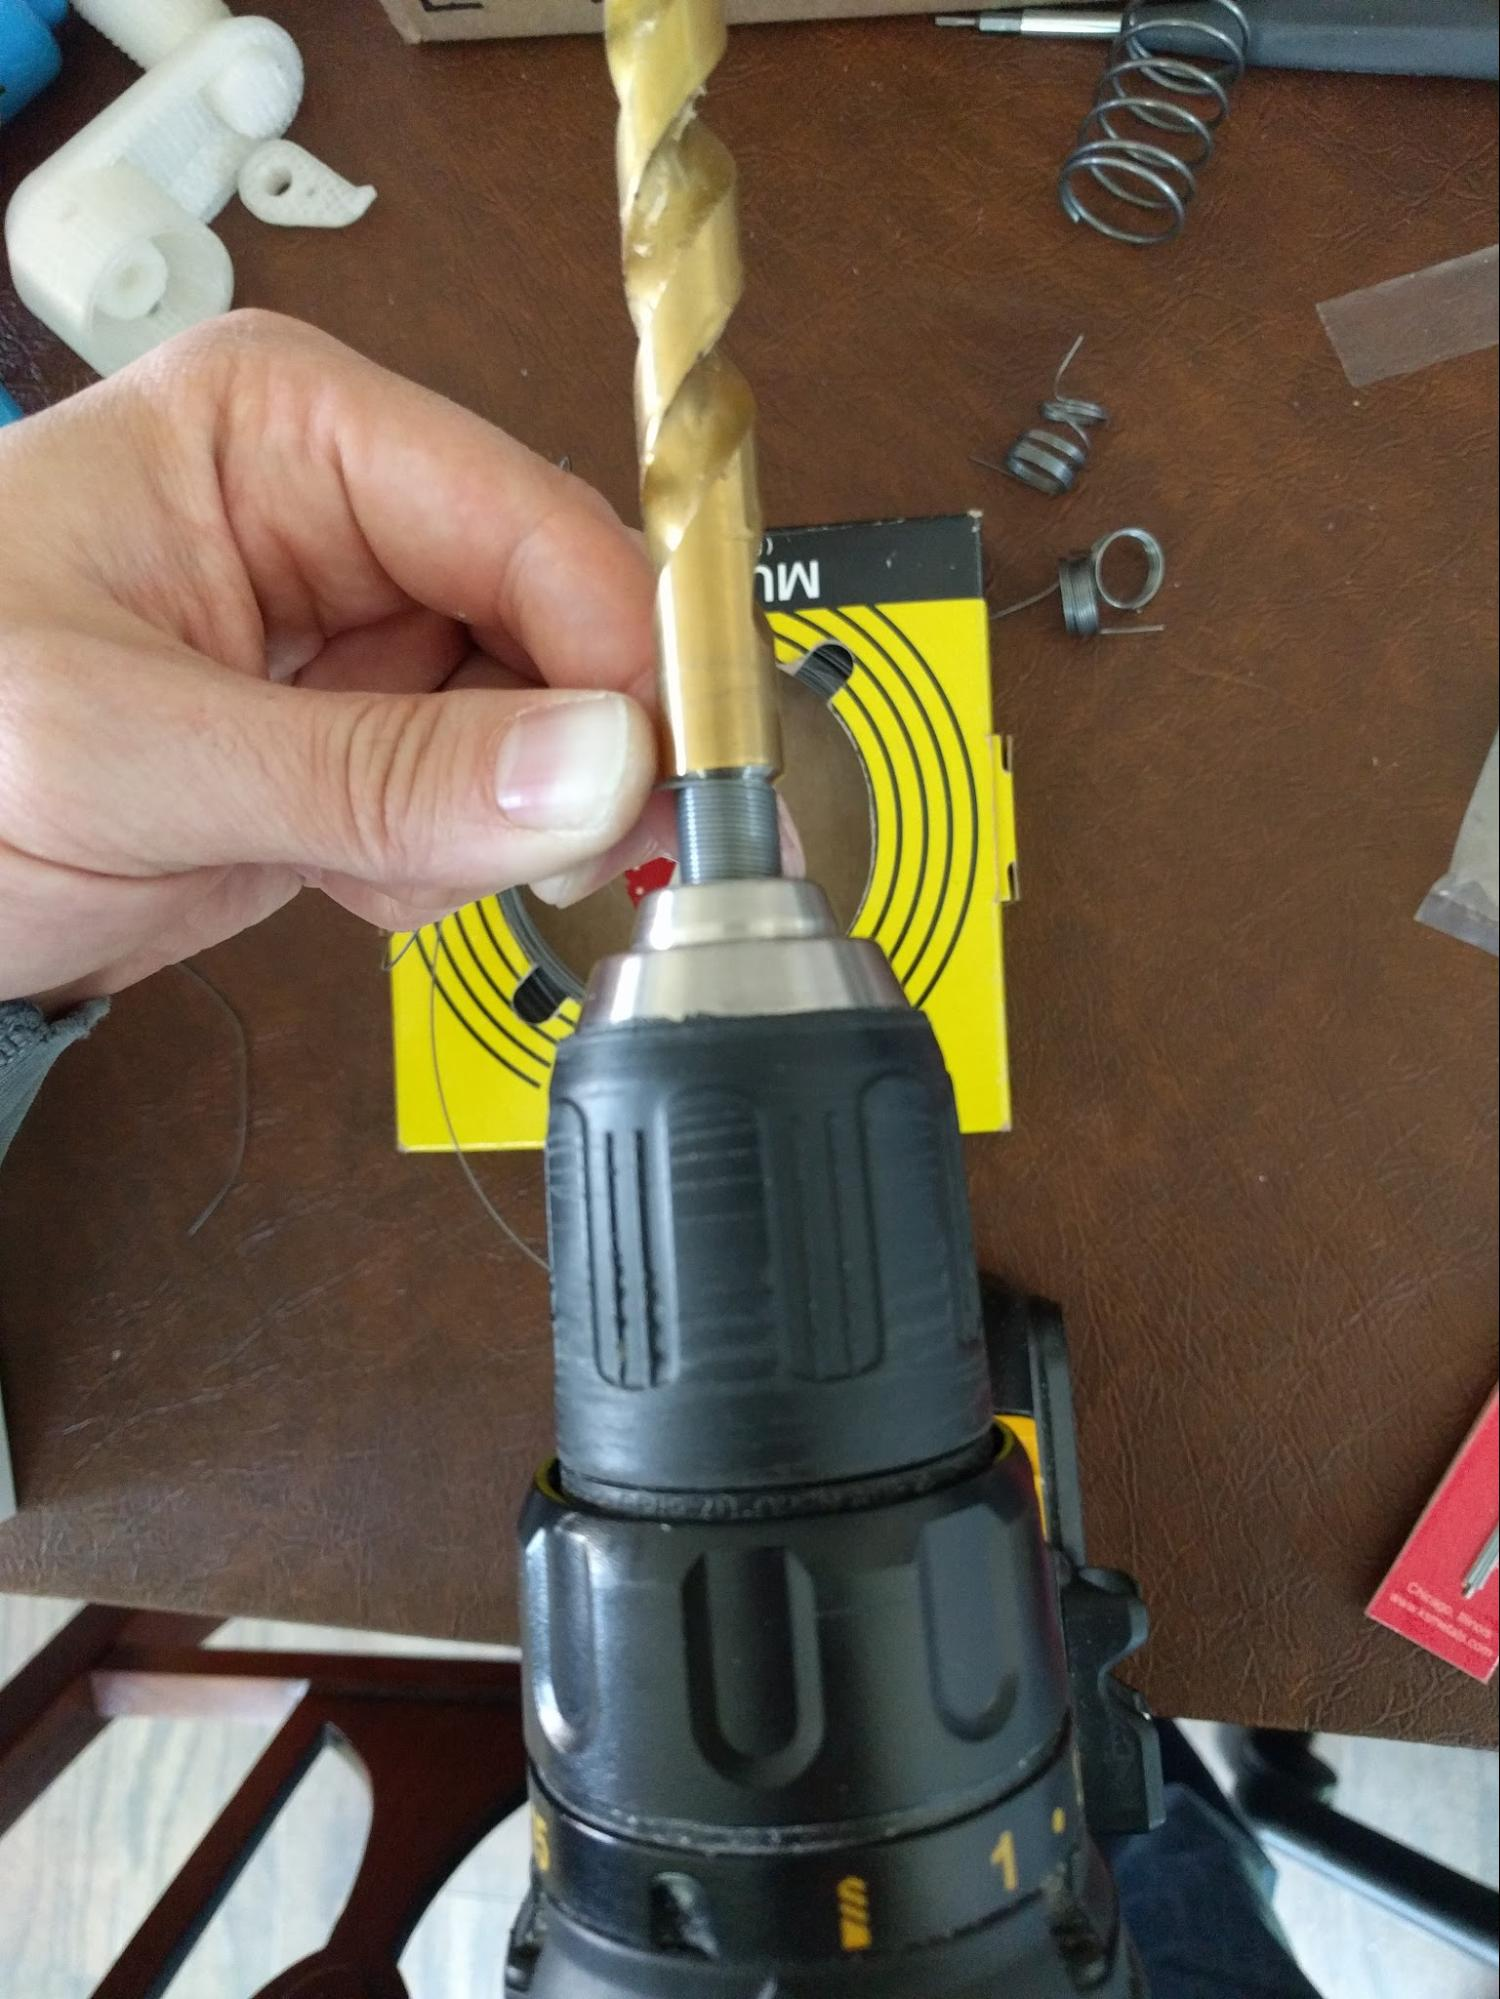
\includegraphics[width=.75\textwidth]{images/image26.jpg}
	\caption{Chucking the drill and wire together to make the spring.}
	\label{fig:image26}	
\end{figure}



\chapter{Zero Positioning Disk}
\section{Parts Required}

\begin{table}[!ht]
	\centering
	\begin{tabular}{clc}
		Part Number & Part Name & Quantity (if $>1$) \\ \hline
		25 & Zero Positioning Disc Roller & \\
		27 & Zero Positioning Disc & \\
		66 & Anti Reversal Pawl (Reverse Rotation Prevention Pawl) & \\
		67 & Zero Positioning Disc Lever & \\
		71 & Main Axle Pin for Zero Positioning Disc & \\
		74 & Zero Positioning Disc Clip (Zero Positioning Plate Securing Spring) & \\
		76 & Zero Positioning Lever Bolt Sleeve & \\
		77 & Anti-Reversal Pawl Bolt Sleeve & \\ \hline \hline
		- & Anti-Reversal Pawl Spring & \\
		- & Zero Positioning Lever Spring & \\ \hline \hline
		1 & M5 hex head 10mm & 1 \\
		2 & M5 hex head 20mm & 1 \\
		3 & M5 hex head 30mm & 1 \\
		4 & M5 nut & 2
	\end{tabular}
\end{table}

\section{Tools Required}
\begin{itemize}
	\item Pliers
	\item Thread lock
	\item Hex wrench sized for M3 bolts
\end{itemize}


\section{Process}
The original Curta design called for shoulder bolts to secure the anti-reversal pawl and the zero positioning lever. Shoulder bolts of the proper size would be difficult to find, so instead sleeves were designed to create shoulder bolts from hex head bolts. The 20mm bolt should be paired with the shorter sleeve while the longer 30mm bolt is paired with the longer sleeve. Now combine the longer bolt / sleeve combination with the zero positioning lever and the shorter bolt / sleeve combination with the anti-reversal pawl. Both of the bolts should easily slide into their sleeves but the hex heads should prevent them from turning relative to the sleeve with little to no filing necessary.

Put the 10mm bolt through the zero positioning lever at the smaller end of the lever with the threads extending in the same direction as the threads for the shoulder bolt. Place the positioning lever roller over the threads of the bolt on the other side of the lever and secure it with thread lock and an M5 nut tightly enough to prevent the roller from wobbling, but loosely enough to allow it to roll easily. The bolt should fit easily through both the lever and the roller with little to no filing necessary.

Slide the larger diameter spring over the zero positioning lever with one leg going through the middle opening in the lever (which hole is used can be played with later to adjust the tension on the positioning lever). Slide the zero positioning lever with its spring into the hole for the zero positioning lever from the bottom side of the bearing plate (refer to Figure \ref{fig:image25}, the diagram of the bearing plate holes). While looking at the bottom of the bearing plate oriented such that the zero positioning lever is at the bottom of the plate, the lever should extend to the right. Add a small amount of thread lock to the threads of an M5 nut and secure the reversing lever from the top side of the bearing plate.

Lift the zero positioning lever away from the main axle and slide the zero positioning disc onto the bottom of the bearing plate. This should fit easily with little to no filing necessary and it should spin freely on the bearing plate. Position the zero positioning disc so that the roller on the positioning lever sits in the recess in the zero positioning disc. Secure the zero positioning disc to the bearing plate with the printed spring clip allowing it to slide into the cutouts in the sleeve of the zero positioning disc, see Figure \ref{fig:image29}. Orient the main axle and step drum to its zero position by ensuring that the step drum can raise and lower. Brace the end of the zero positioning disc against a solid object and use the flat edge of a tool (the side of some pliers should do) to hammer the main axle pin in place, see Figure \ref{fig:mainaxlepin}. This should be a tight fit, but also shouldn’t require too much force (don’t break anything). If it does, file down the pin some. 

\begin{figure}[!ht]
	\centering
	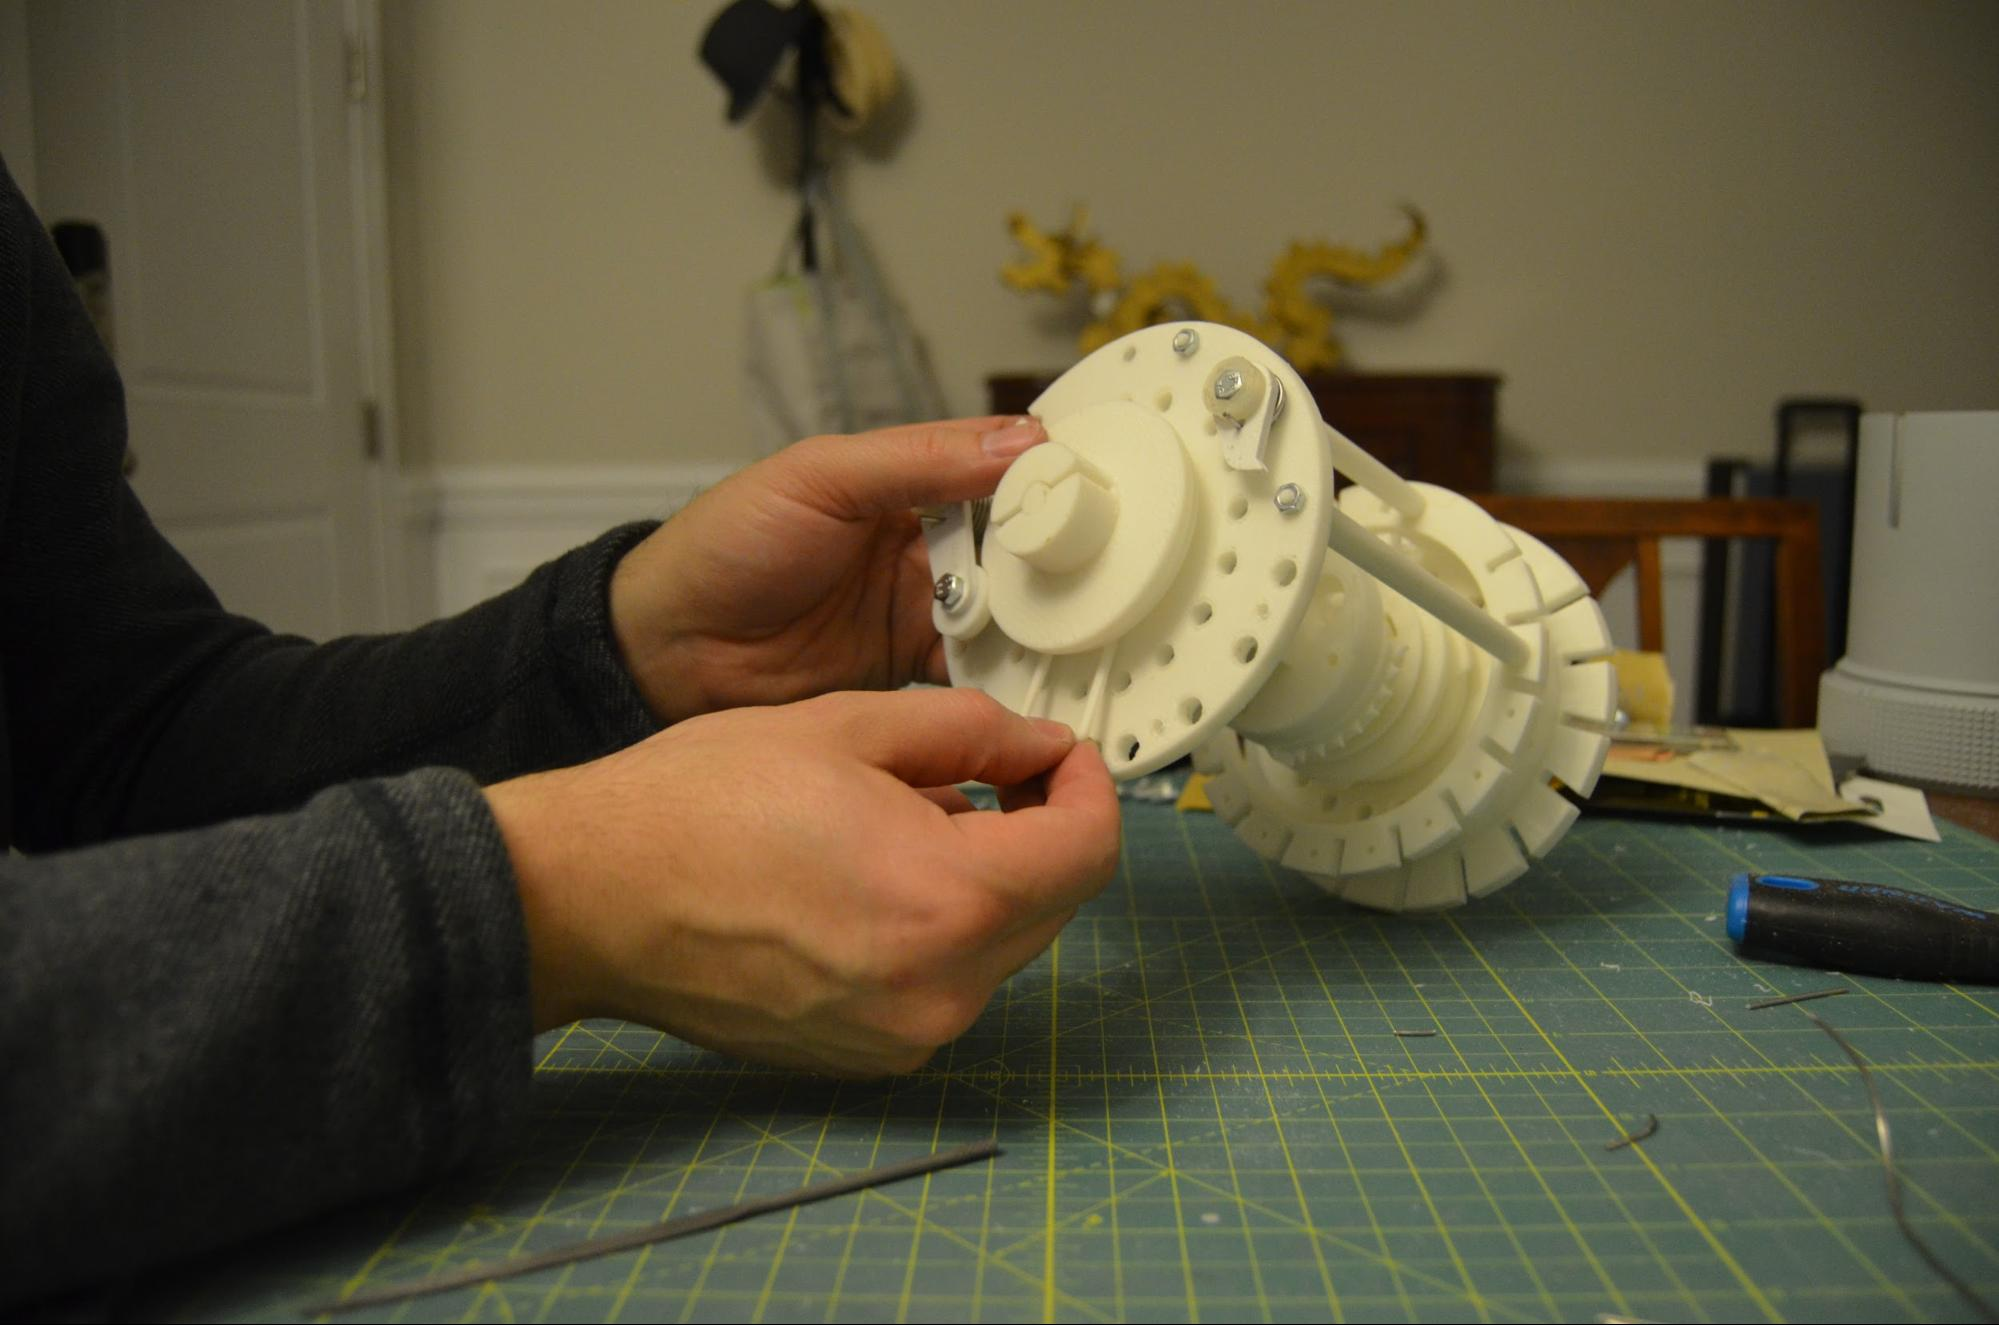
\includegraphics[width=.75\textwidth]{images/image29.jpg}
	\caption{Placing the Zero Positioning Disc Clip to secure the Zero Positioning Disc to the Bearing Plate.}
	\label{fig:image29}	
\end{figure}


\begin{figure}[!ht]
	\centering
	\begin{subfigure}{.45\textwidth}
		\centering
		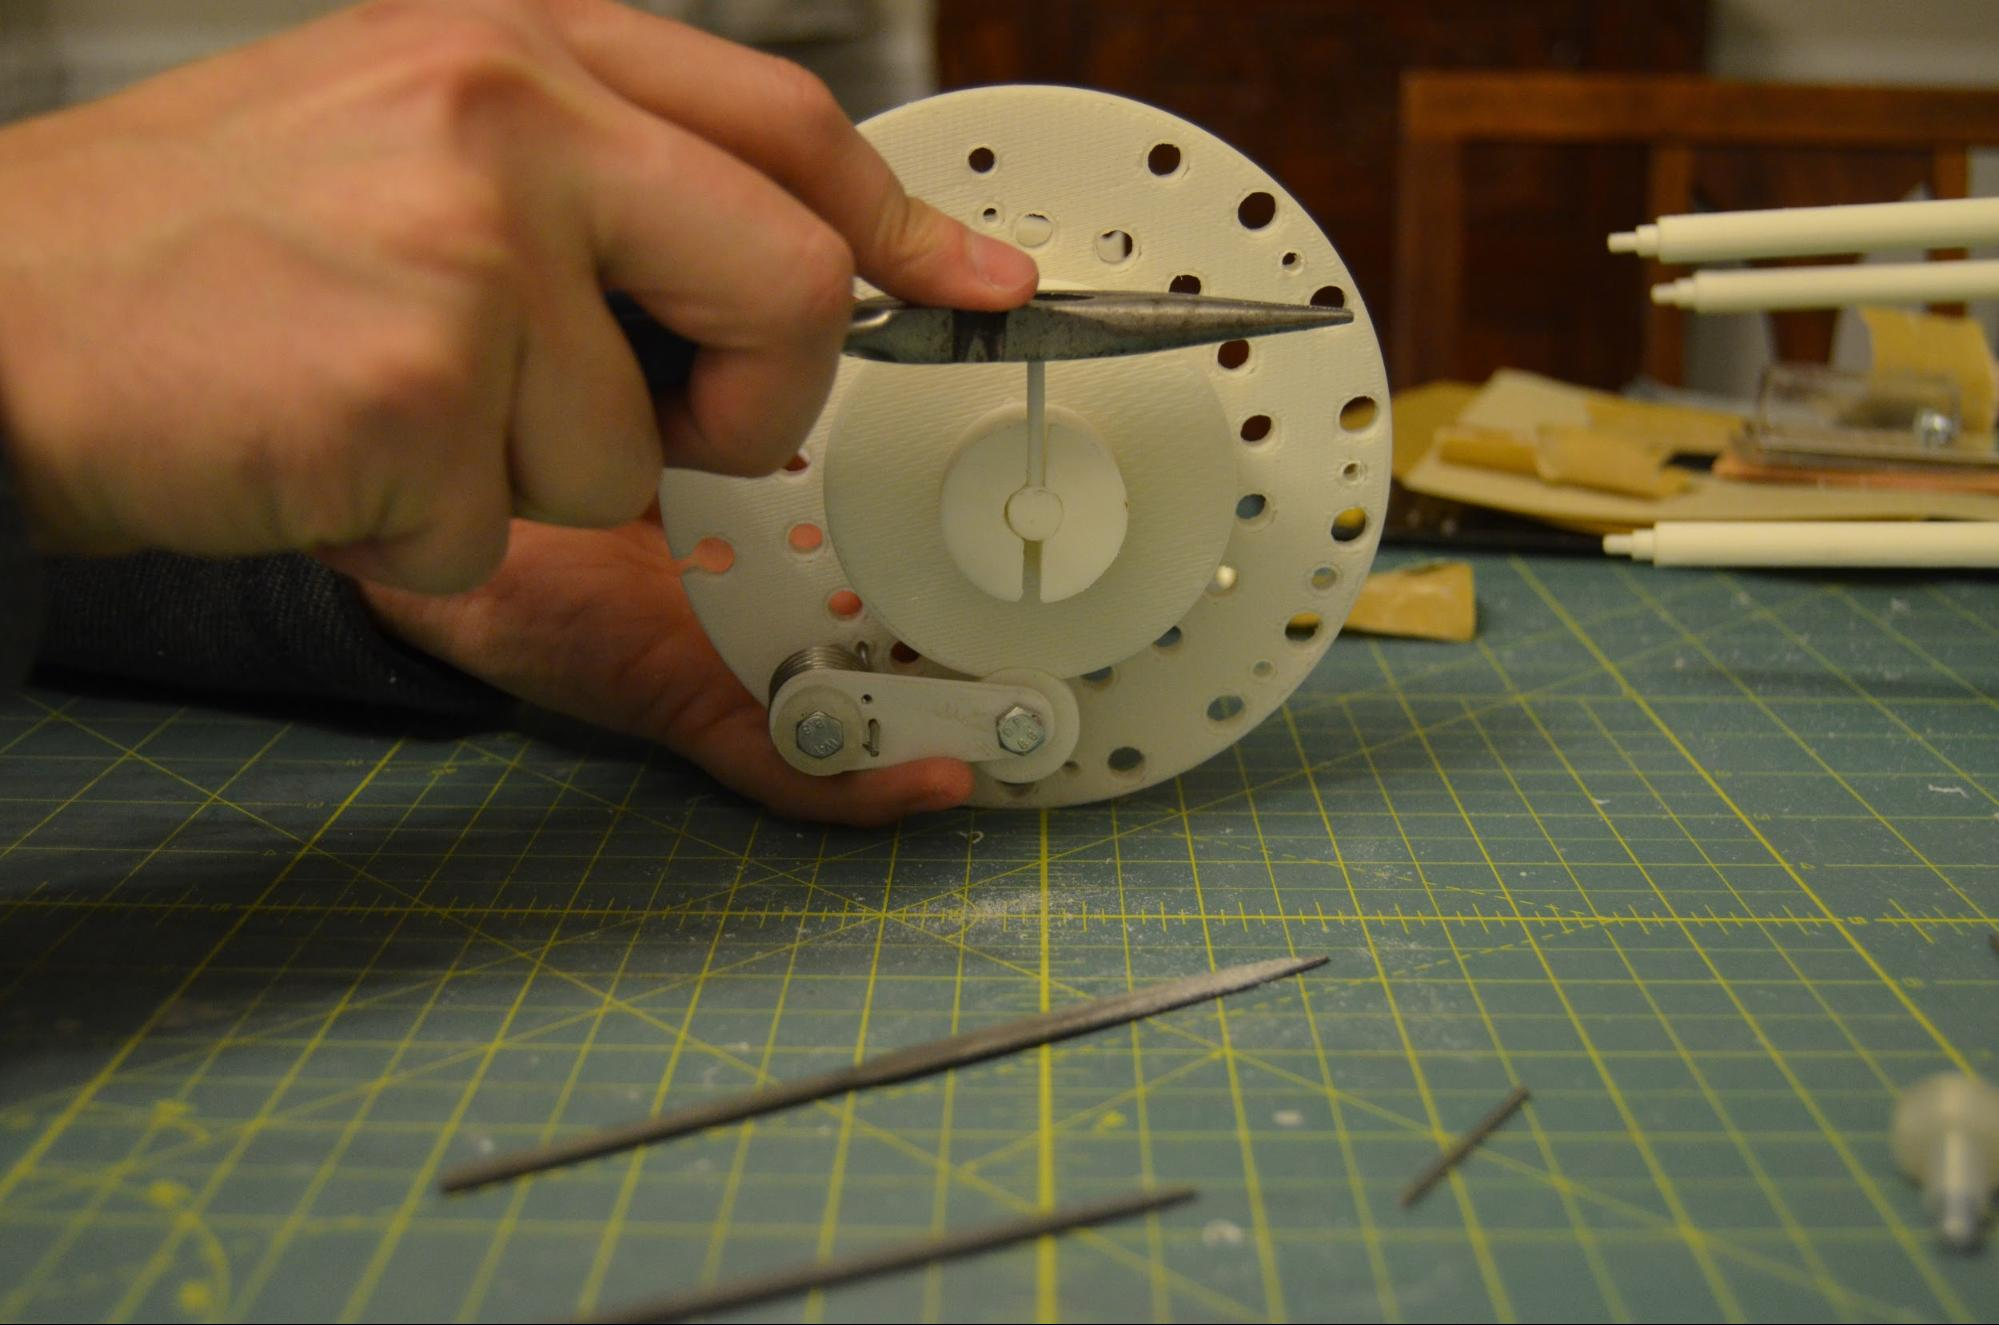
\includegraphics[width=.9\textwidth]{images/image18.jpg}
		%\caption{Image 18}
		\label{fig:image18}	
	\end{subfigure}
	\begin{subfigure}{.45\textwidth}
		\centering
		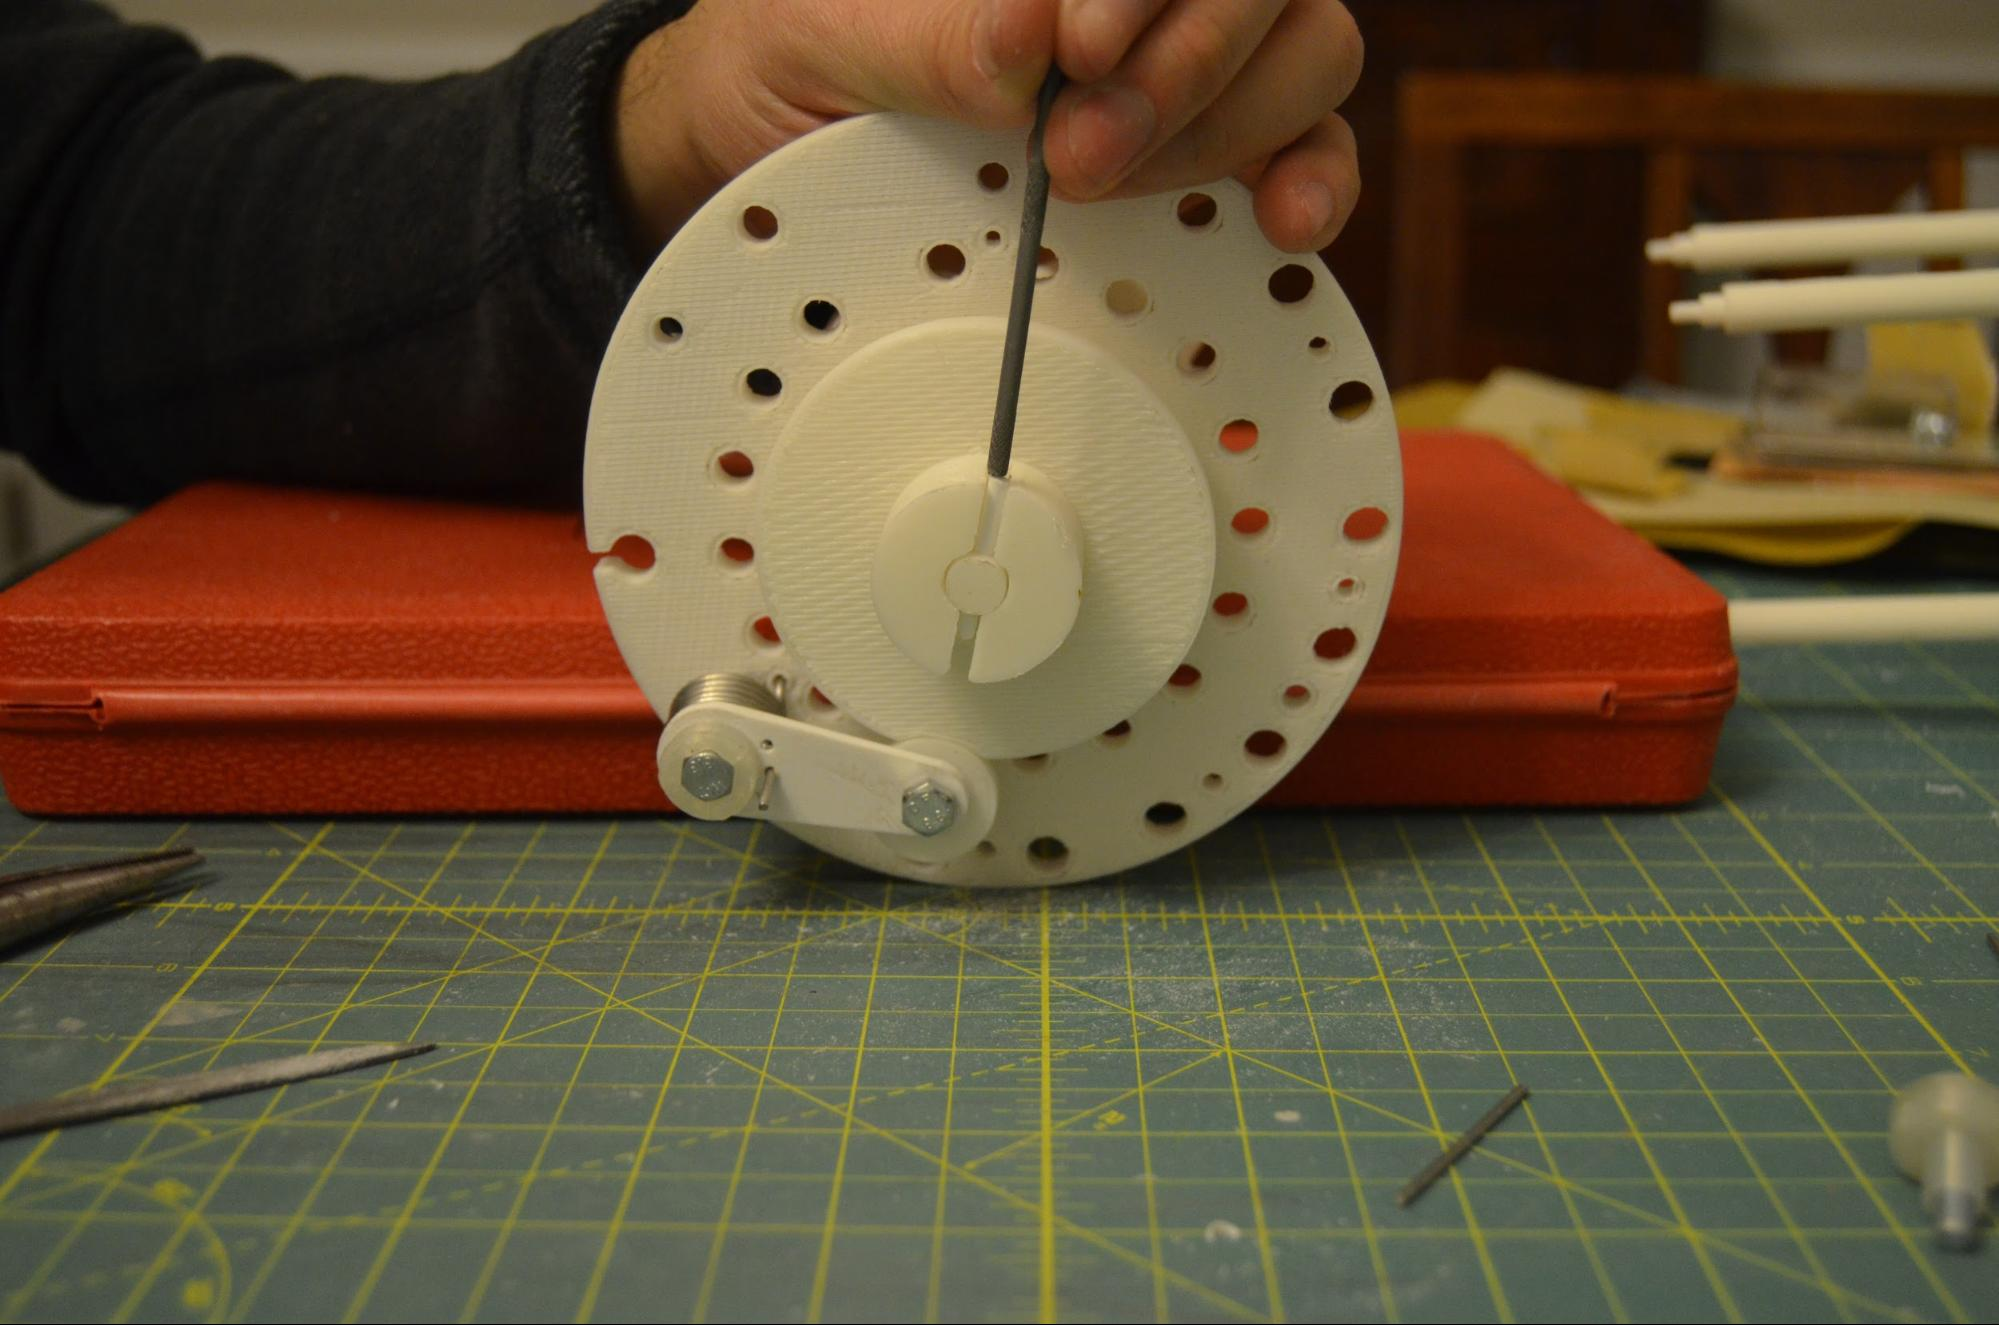
\includegraphics[width=.9\textwidth]{images/image3.jpg}
		%\caption{Image 3}
		\label{fig:image3}	
	\end{subfigure}
	\caption{Securing the Tens Bell with the Main Axle Pin.}
	\label{fig:mainaxlepin}
\end{figure}


Place the hex wrench into the hole at the top of the step drum and give the step drum a few rotations. It should turn easily (though probably with a small increase in friction than before) and the stop at the zero position should be clearly noticeable. If it does not turn easily, take the zero positioning lever and disc off and file down any irregularities. Take note of any bumps or unevenness on the bottom of the bearing plate and the inside of the zero positioning disc.

Slide the smaller diameter spring over the anti-reversal pawl with one leg sliding into the hole in it. Thread the anti-reversal pawl into the bottom side of the bearing plate (the same side as the zero positioning lever) making sure that the pointed edge of the pawl interfaces with the teeth on the zero positioning disc and the other leg of the spring slides into the hole for it in the bearing plate. Test the pawl by quickly moving a small screwdriver or other thin tool between the pawl and the zero positioning disc at a tangent to the disc. It should lift the pawl away from the teeth until the tool moves past the pawl and then the spring should snap the pawl back to the teeth of the disc. This should require minimal force. If the pawl doesn’t return to the zero positioning disc, check that the spring isn’t caught between the bottom of the pawl and the bearing plate. 

Once again, use a hex wrench through the top hole of the step drum to turn the step drum a few times. It should still turn easily but now it should only turn clockwise. Check (with light pressure) that it doesn’t turn in reverse.



\chapter{Main Casting and Bearing Plate}
\section{Parts Required}
\begin{table}[!ht]
	\centering
	\begin{tabular}{clc}
		Part Number & Part Name & Quantity (if $>1$) \\ \hline
		- & Assembled Main Casting and Tens Bell with Support Columns & \\
		- & Assembled Bearing Plate, Main Axle, and Step Drum & \\ \hline \hline
		8 & M4 nuts & 3
	\end{tabular}
\end{table}

\section{Tools Required}
\begin{itemize}
	\item Pliers or open ended 4mm wrench
\end{itemize}


\section{Process}
In a previous step, the support columns should already have both ends threaded and should have already been test-fit to the bearing plate. The main shaft should have also been test fit in the tens bell. It is easier to do those steps earlier rather than now since so many parts are coming together.

Slide the main casting over the main axle until the support columns meet the bearing plate. Turn the bearing plate until the holes for the support columns align with the support columns. Press the bearing plate onto the support columns, then secure each column with an M4 nut.

\begin{figure}[!ht]
	\centering
	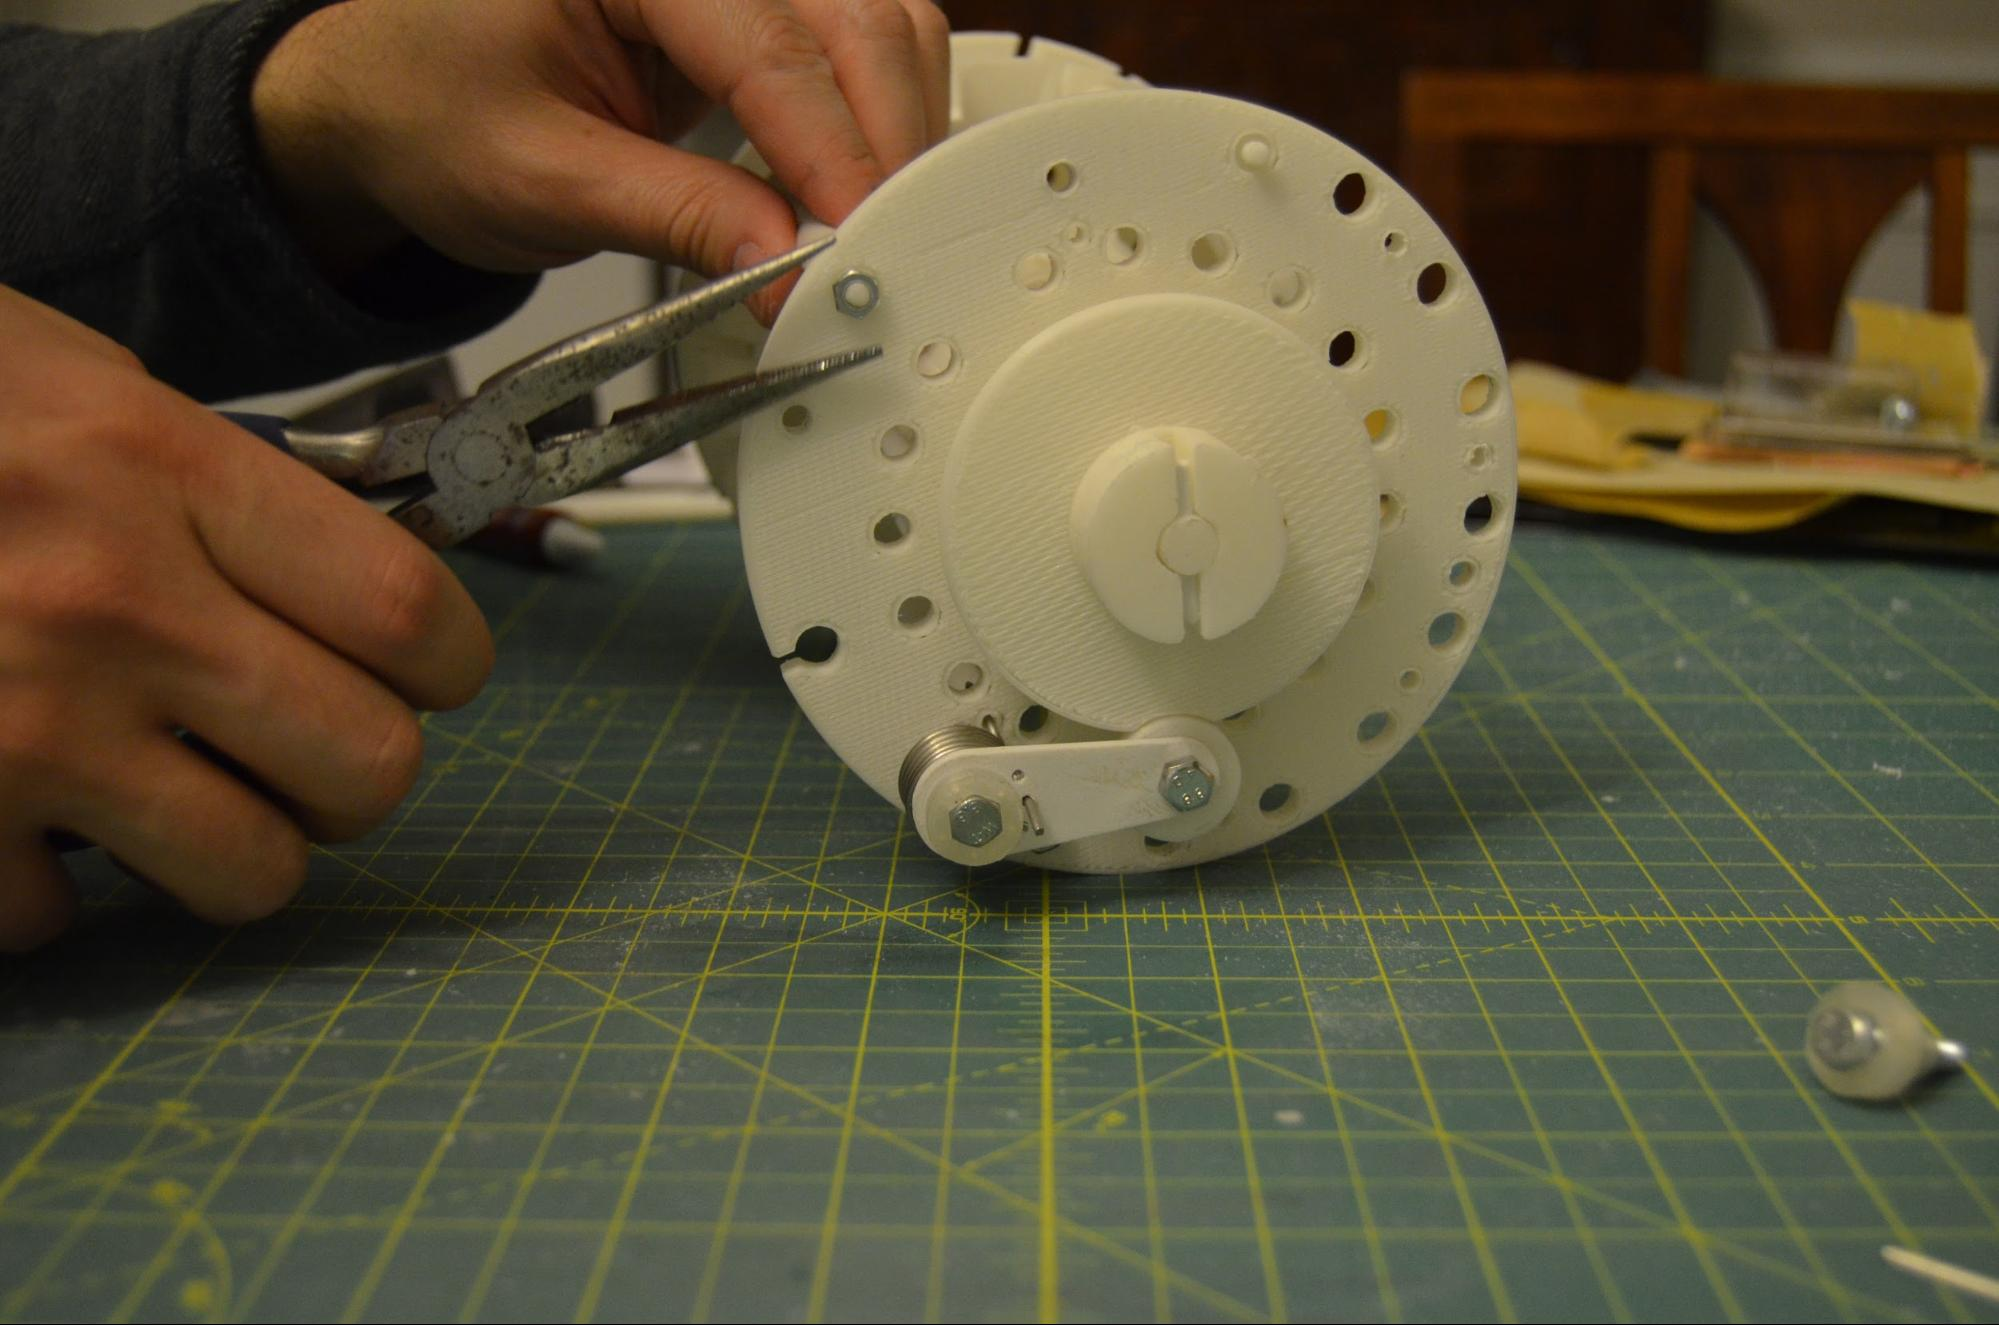
\includegraphics[width=.75\textwidth]{images/image32.jpg}
	\caption{Securing Support Columns to the Bearing Plate.}
	\label{fig:image32}	
\end{figure}


Double-check that the main axle can shift up and down in the zero position, that it cannot when mid-turn, that the main axle turns easily, and that it does not turn in reverse. If there is a significant increase in friction, backtrack one step at a time until the source of the friction is found. Additional filing to fit parts or spray lubricant may be necessary.




\chapter{Transmission Shafts}
\section{Parts Required}
\begin{table}[!ht]
	\centering
	\begin{tabular}{clc}
		Part Number & Part Name & Quantity (if $>1$) \\ \hline
		6 & Double Transmission Gear &  \\
		7 & Standard Transmission Gear & 15 \\
		8 & Lockout &  \\
		9 & Triple Transmission Gear & \\
		10 & Tall Lockout & \\
		11 & Lockout with Transmission Gear & 15 \\
		28 & Ones Results Transmission Shaft & \\
		29 & Ones Turns Transmission Shaft & \\
		30 & Transmission Shaft & 12 \\
		31 & 9, 10, 11 Digits Transmission Shaft & 3 \\
		59 & Transmission Lock Ring (Cover Ring) & \\ \hline \hline
		11 & M3 10mm Screws & 3
	\end{tabular}
\end{table}

\section{Tools Required}
\begin{itemize} 
	\item Thread lock
\end{itemize}

\section{Process}
It's important to know the difference between the transmission gears and lockouts. Switching these
parts will cause the Curta to either not rotate properly or to break. Figure \ref{fig:transmission:dif}
shows a top-down profile of both a gear and lockout. Note that some transmission gears have both
gears and lockouts. 

\begin{figure}[!ht]
	\centering
	\begin{subfigure}{.4\textwidth}
		\centering
		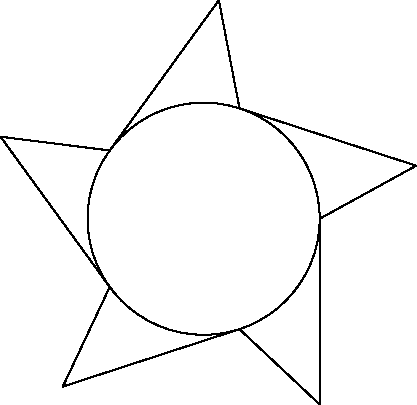
\includegraphics[width=.45\textwidth]{images/transmission-gear.pdf}
		\caption{Transmission Gear}
	\end{subfigure}
	\begin{subfigure}{.4\textwidth}
		\centering
		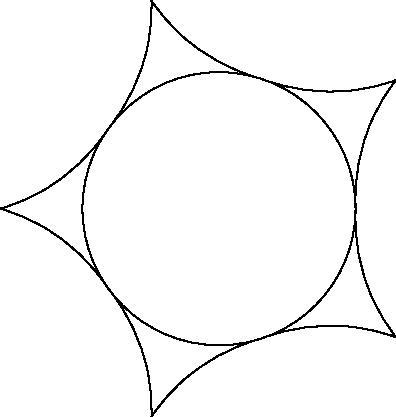
\includegraphics[width=.45\textwidth]{images/transmission-lockout.pdf}
		\caption{Transmission Lockout}
	\end{subfigure}
	\caption{Comparing gears and lockout.}
	\label{fig:transmission:dif}
\end{figure}



Additionally, be sure to orient the gears correctly. If they are placed upside down, they will not turn properly. One easy way to know is that the tab on the inside that slots into the groove in the transmission shaft starts at the base, but does not reach all the way to the top. Figure \ref{fig:gearorient} shows the orientation of the gears.

\begin{figure}[!ht]
	\centering
	\begin{subfigure}{.46\textwidth}
		\centering
		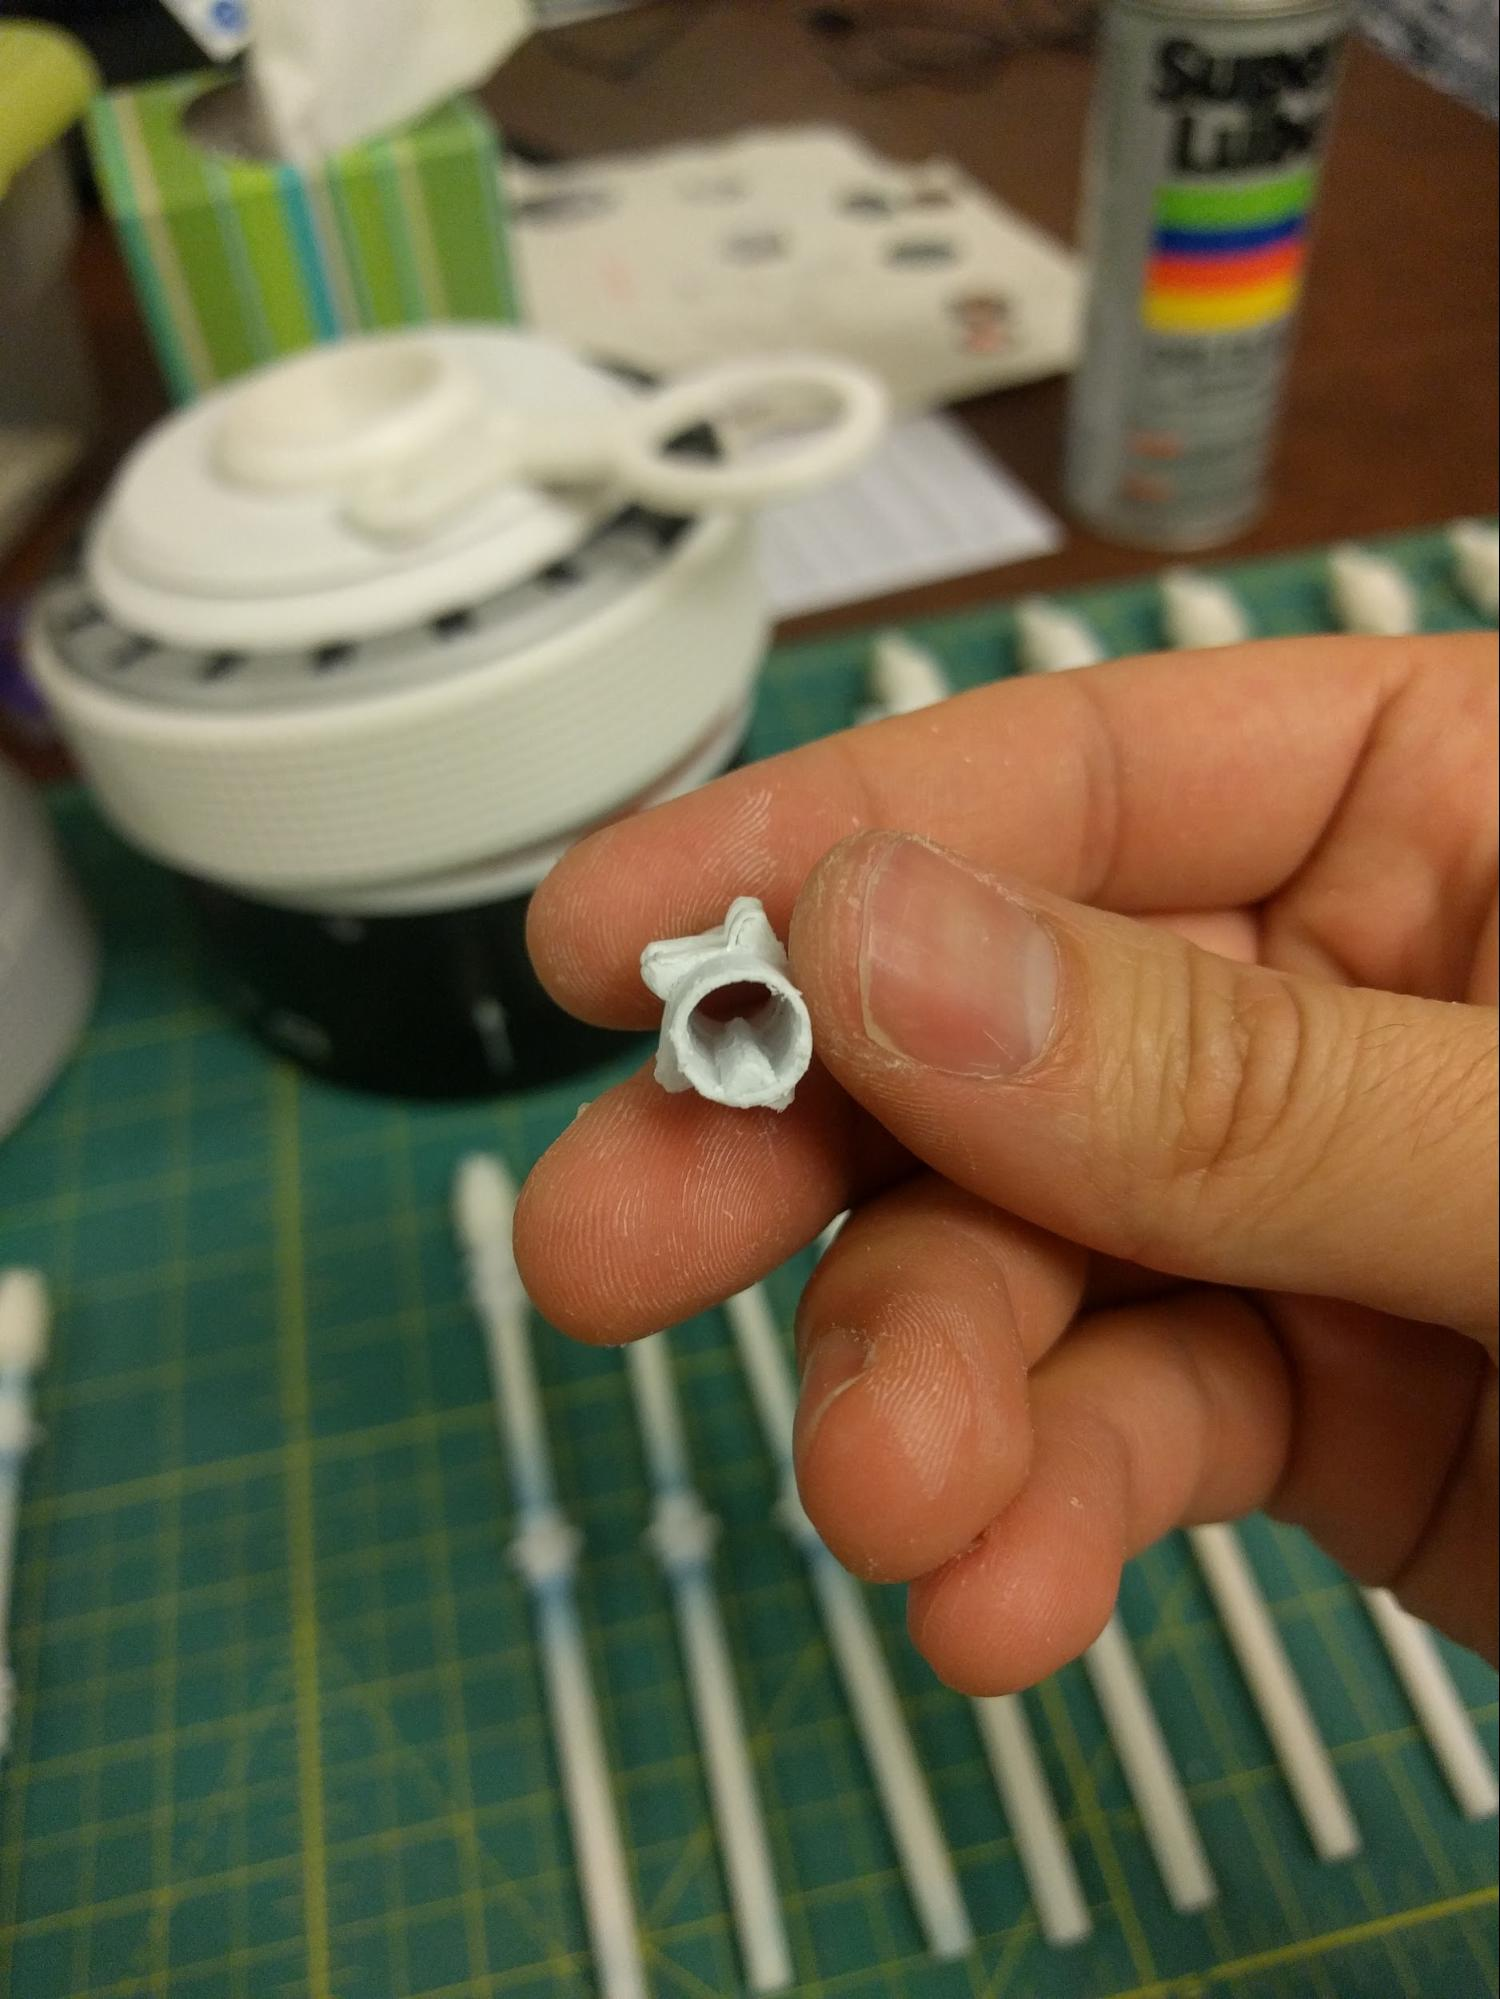
\includegraphics[width=.95\textwidth]{images/image56.jpg}
		\caption{Bottom of the gears, should face the bearing plate.}
		\label{fig:image56}	
	\end{subfigure}
	\begin{subfigure}{.46\textwidth}
		\centering
		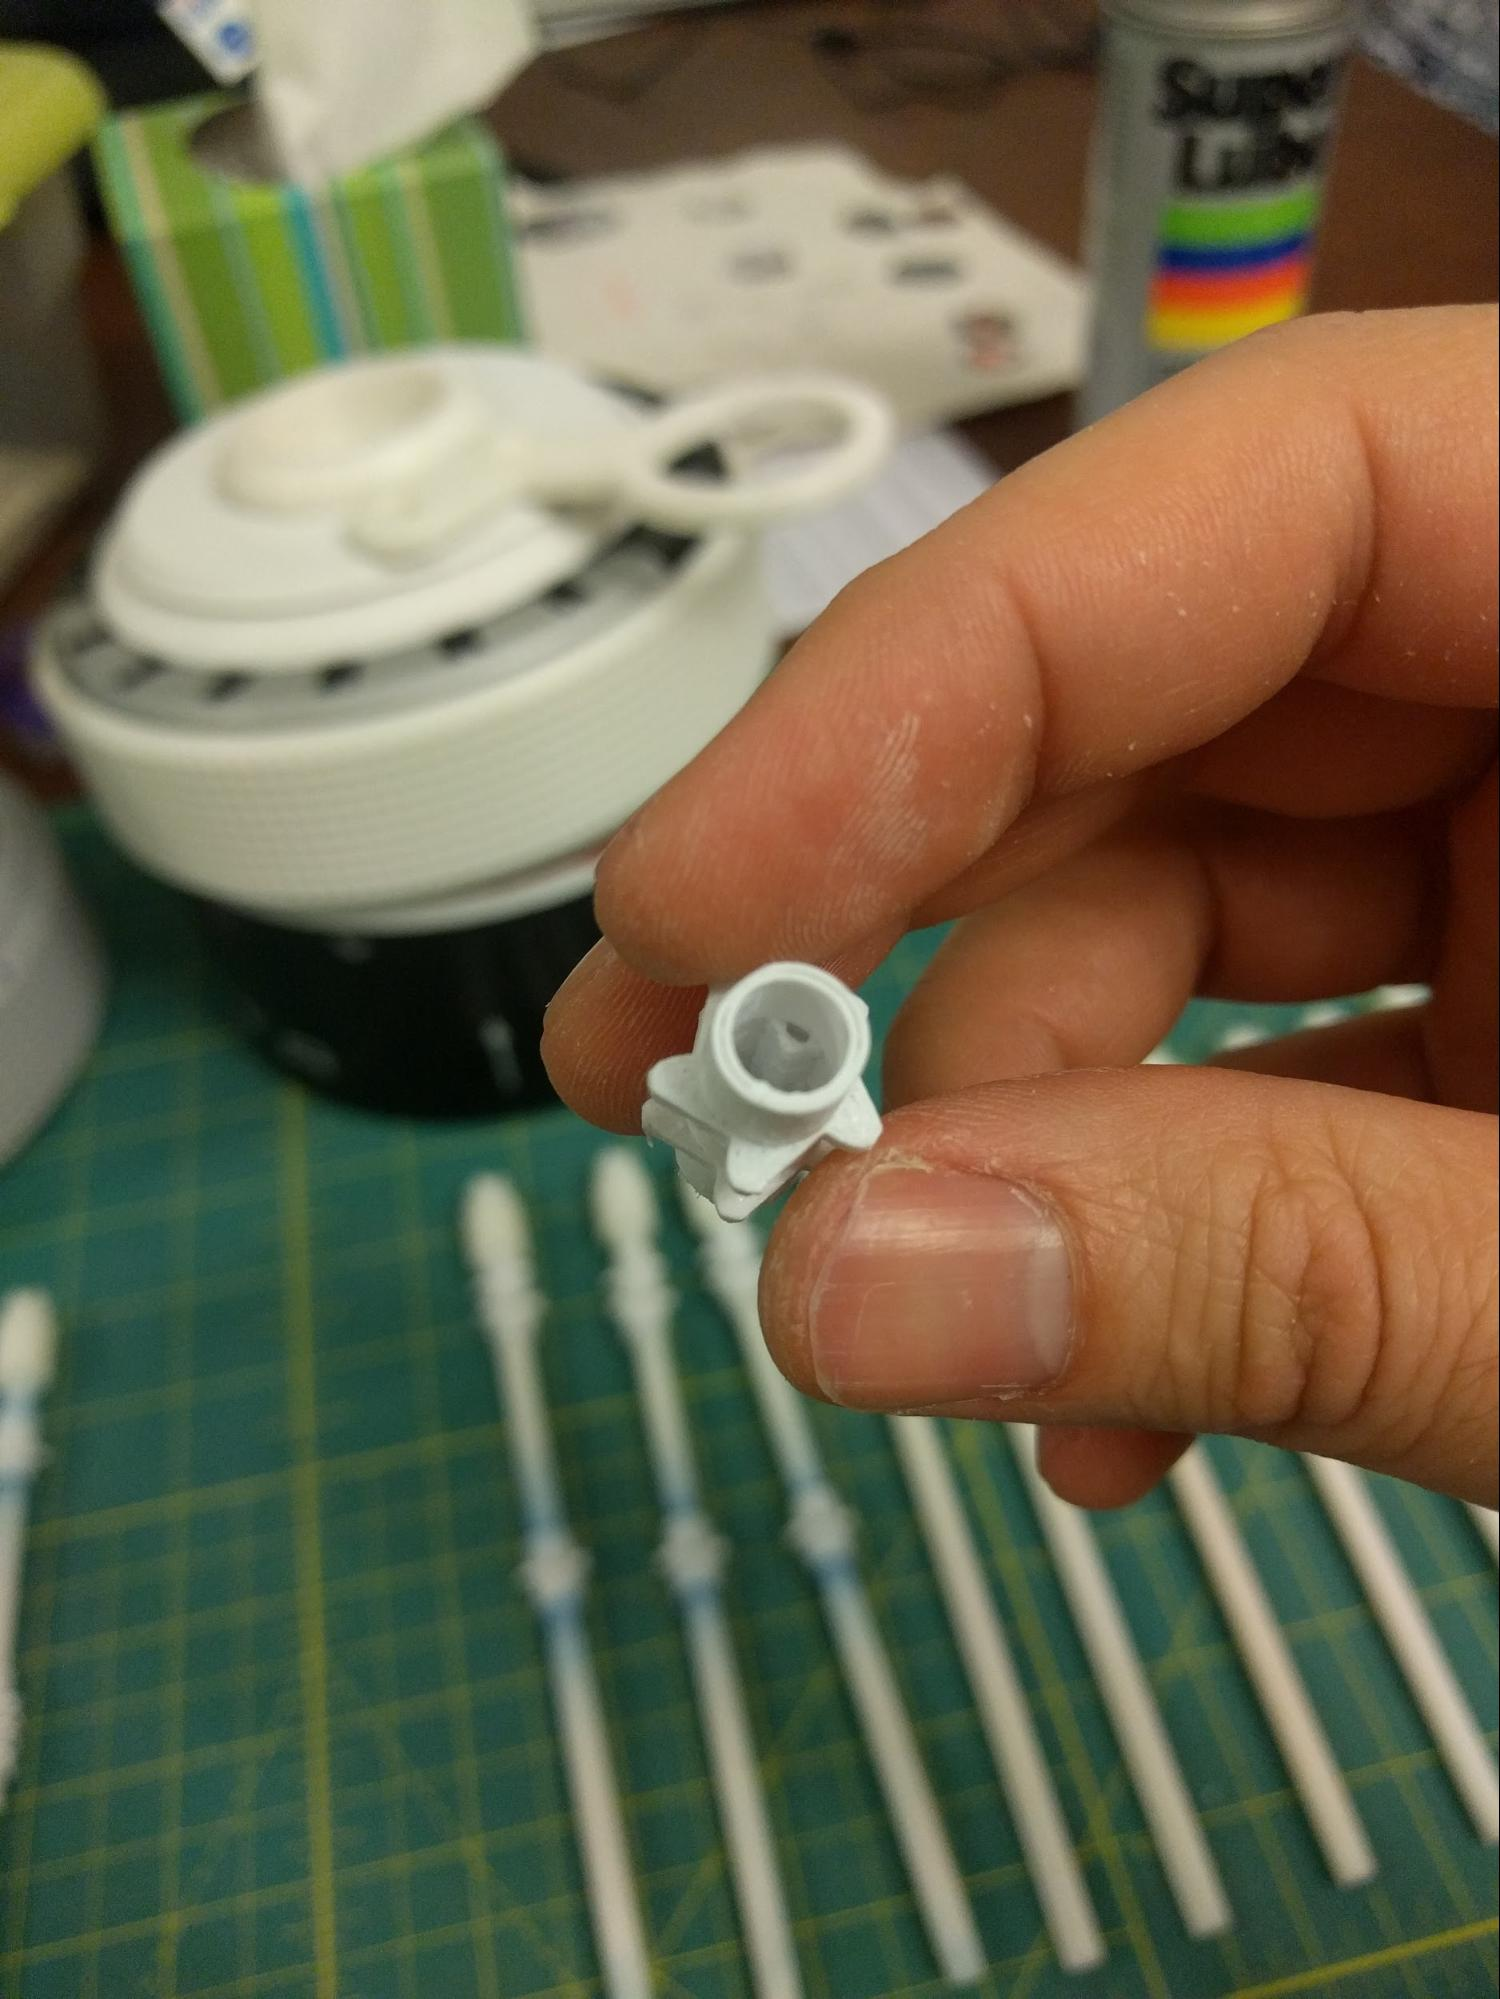
\includegraphics[width=.95\textwidth]{images/image38.jpg}
		\caption{Top of the gears, should face the main casting.}
		\label{fig:image38}	
	\end{subfigure}
 	\caption{Be sure to orient the gears correctly}
 	\label{fig:gearorient}
\end{figure}




There are 4 distinct transmission shaft types, and each type gets a specific set of gears. Figure
\ref{fig:transmission:gearlayout} shows each shaft type and what gears they receive, and their relative
order (this is also described below). Some of the gears must be secured in place. The original Curta uses small clips, but the printed equivalents did not stay in place so thread lock is used. What is great about it is that it still allows disassembly and reassembly. Apply the thread lock and let it dry completely, then carefully disassemble and reassemble in the Curta. Disassembly will be tough, but should yield parts that hold together snugly.
Figure \ref{fig:image24} shows the process of securing with threadlock.


\begin{figure}[!ht]
	\centering
	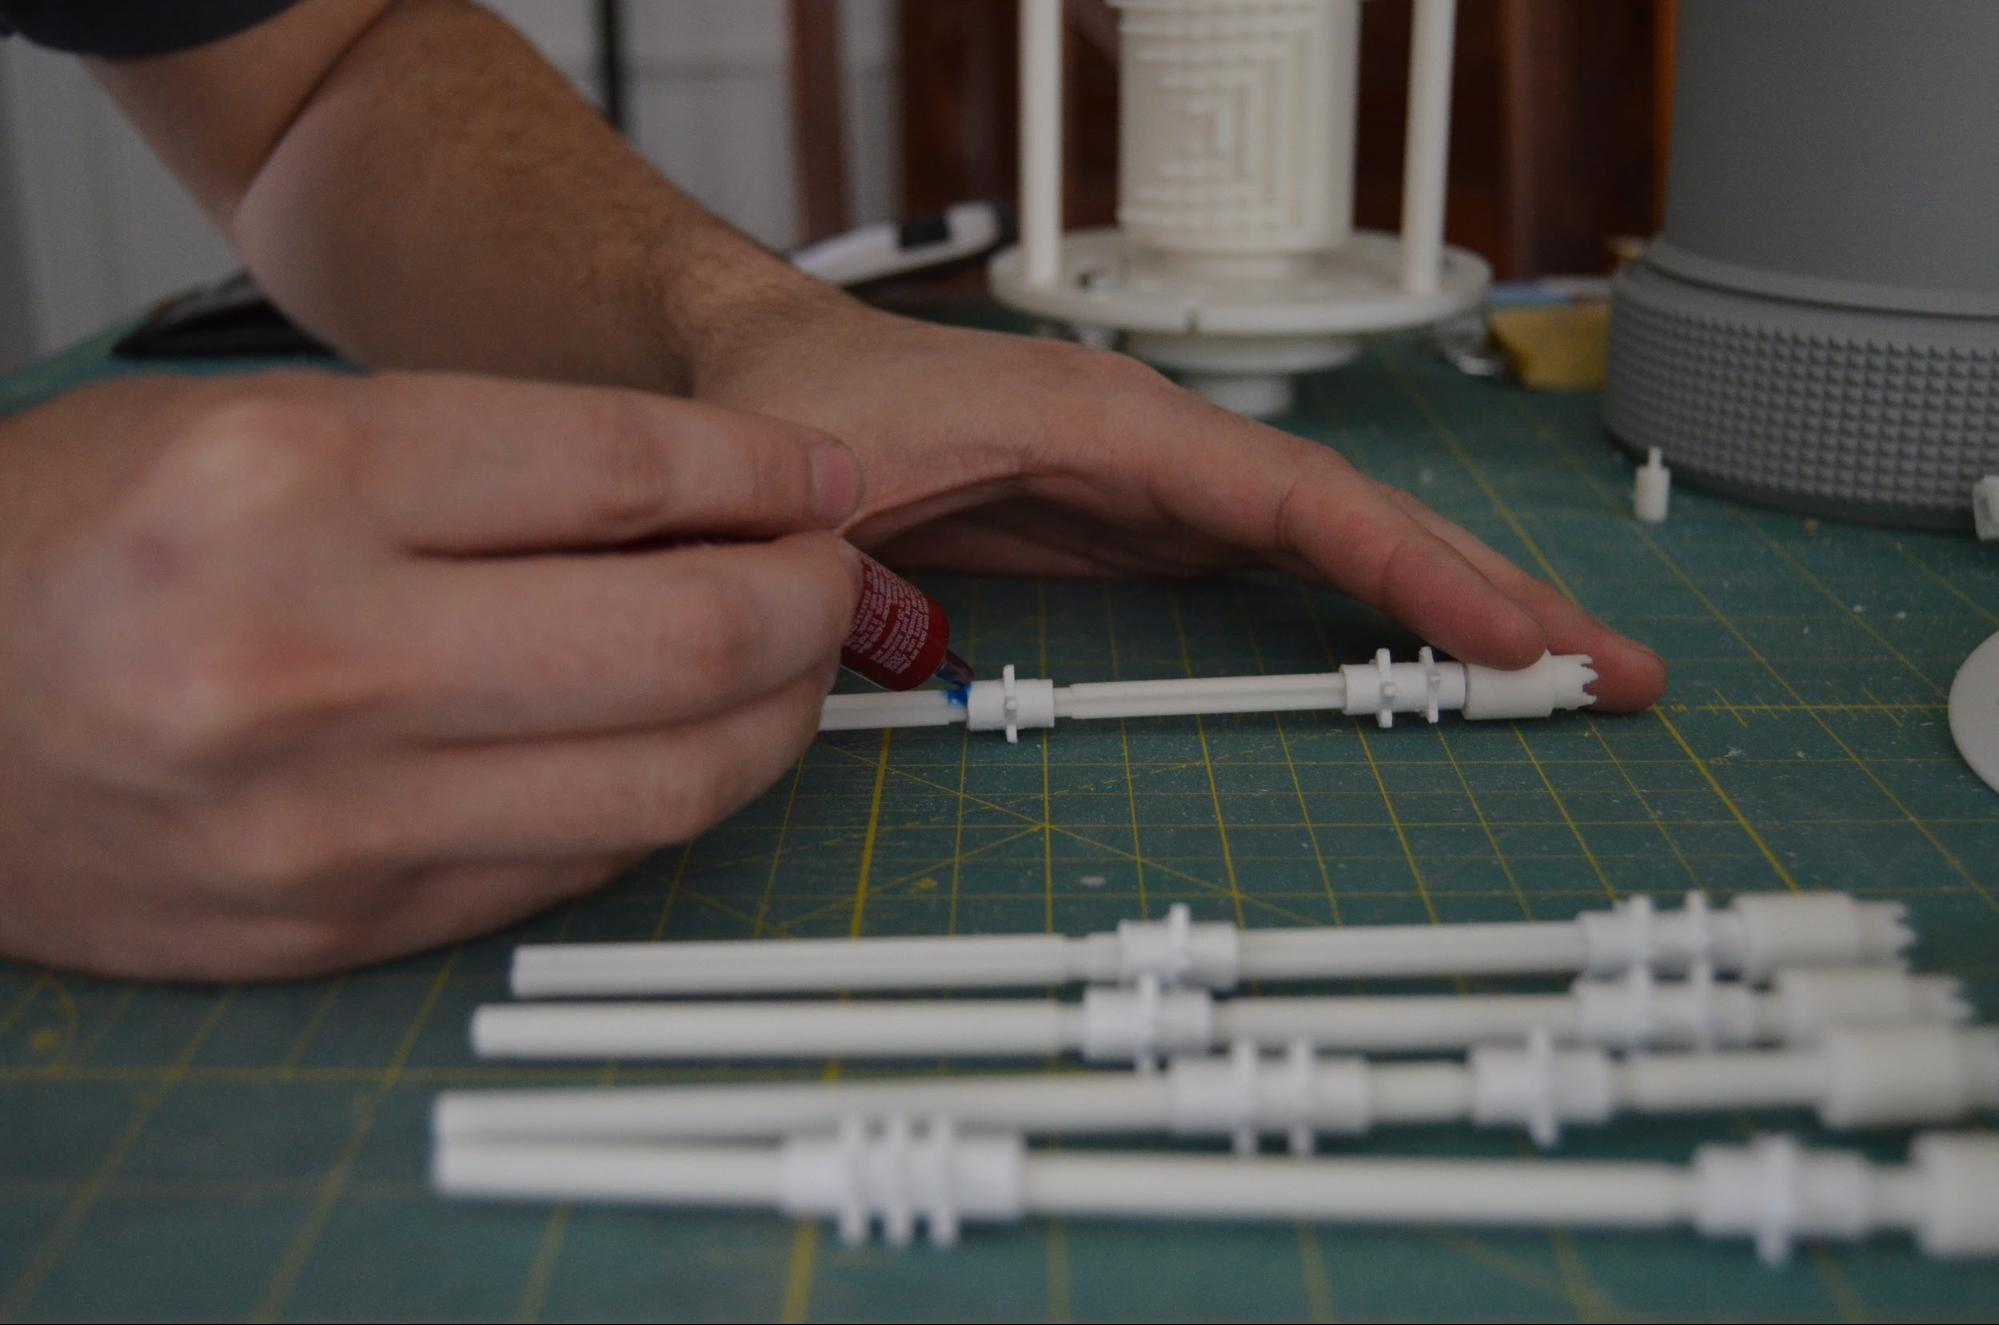
\includegraphics[width=.75\textwidth]{images/image24.jpg}
	\caption{Applying thread lock to secure the gears.}
	\label{fig:image24}	
\end{figure}



\begin{itemize}
 \item The transmission shafts (part 30, Fig \ref{fig:transmission:shaftgear}) receive a lockout 
with transmission gear (part 11) and a standard transmission gear (7).
 \item The 9, 10 ,11 digit transmission shafts (part 31, Fig \ref{fig:transmission:9gear}) receive a lockout with transmission gear (part 11) and a standard transmission gear (7), this gear should be
secured in place.
 \item The ones result transmission shaft (part 28, Fig \ref{fig:transmission:resultgear}) receives a
lockout (8) secured in place and a double transmission gear (6).
 \item The ones turns transmission shaft (part 29, Fig \ref{fig:transmission:turnsgear}) receives a 
tall lockout (10) secured in place and a triple transmission gear (9).
\end{itemize}

\begin{figure}[!ht]
	\centering
	\begin{subfigure}{.2\textwidth}
		\centering
		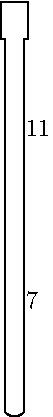
\includegraphics[scale=1]{images/transmission-shaft-gear.pdf}
		\caption{30 - T Shaft}
		\label{fig:transmission:shaftgear}	
	\end{subfigure}
	\begin{subfigure}{.2\textwidth}
		\centering
		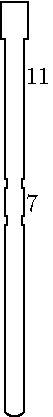
\includegraphics[scale=1]{images/transmission-result-9-gear.pdf}
		\caption{31 - 9, 10, 11 T}
		\label{fig:transmission:9gear}	
	\end{subfigure}
	\begin{subfigure}{.2\textwidth}
		\centering
		
\includegraphics[scale=1]{images/transmission-result-one-gear.pdf}
		\caption{28 - One Result}
		\label{fig:transmission:resultgear}	
	\end{subfigure}
	\begin{subfigure}{.2\textwidth}
		\centering
		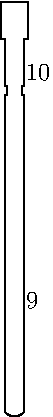
\includegraphics[scale=1]{images/transmission-turns-one-gear.pdf}
		\caption{29 - One Turn}
		\label{fig:transmission:turnsgear}	
	\end{subfigure}
	\caption{Gear layout on the transmission shafts.}
	\label{fig:transmission:gearlayout}
\end{figure}



Figure \ref{fig:transmission} shows the configurations of the results and turns counter transmission shafts. The results set is larger. They are both oriented with the smallest significant digit to the right and largest to the left -- the same order they go in the Curta. Figure \ref{fig:transmission}
shows a full color layout of the shafts with each gear in the correct location and secured in place.
At this point double check to be sure you didn't switch a gear with a lockout and your gears 
are in the correct order.



\begin{figure}[!ht]
	\centering
	\begin{subfigure}{.4\textwidth}
		\centering
		
\includegraphics[width=.05\textwidth]{images/transmission-result-9.pdf}\, 
		
\includegraphics[width=.05\textwidth]{images/transmission-result-9.pdf}\,
		
\includegraphics[width=.05\textwidth]{images/transmission-result-9.pdf}\,
		
\includegraphics[width=.05\textwidth]{images/transmission-shaft.pdf}\,
		
\includegraphics[width=.05\textwidth]{images/transmission-shaft.pdf}\,
		
\includegraphics[width=.05\textwidth]{images/transmission-shaft.pdf}\,
		
\includegraphics[width=.05\textwidth]{images/transmission-shaft.pdf}\,
		
\includegraphics[width=.05\textwidth]{images/transmission-shaft.pdf}\,
		
\includegraphics[width=.05\textwidth]{images/transmission-shaft.pdf}\,
		
\includegraphics[width=.05\textwidth]{images/transmission-shaft.pdf}\,
		
\includegraphics[width=.05\textwidth]{images/transmission-result-one.pdf}
		\caption{Results Shafts}
	\end{subfigure}
	\begin{subfigure}{.4\textwidth}
		\centering
    		
\includegraphics[width=.05\textwidth]{images/transmission-shaft.pdf}\,
		
\includegraphics[width=.05\textwidth]{images/transmission-shaft.pdf}\,
		
\includegraphics[width=.05\textwidth]{images/transmission-shaft.pdf}\,
		
\includegraphics[width=.05\textwidth]{images/transmission-shaft.pdf}\,
		
\includegraphics[width=.05\textwidth]{images/transmission-shaft.pdf}\, 
		
\includegraphics[width=.05\textwidth]{images/transmission-turns-one.pdf}  
		\caption{Turns Counters}
	\end{subfigure}
	\caption{Layout of the transmission shafts, notice the notches on some shafts.}
	\label{fig:transmission:shafts}
\end{figure}







\begin{figure}[!ht]
	\centering
	\begin{subfigure}{.4\textwidth}
		\centering
		\includegraphics[width=.95\textwidth]{images/image21.jpg}
		\caption{Results Shafts}
		\label{fig:image21}	
	\end{subfigure}
	\begin{subfigure}{.4\textwidth}
		\centering
		\includegraphics[width=.95\textwidth]{images/image40.jpg}
		\caption{Turns Counters}
		\label{fig:image40}	
	\end{subfigure}
	\caption{Transmission Shafts}
	\label{fig:transmission}
\end{figure}


%The first results transmission shaft has two recessed sections near the top. A rotation lockout segment %goes there and a double gear sleeve slides on underneath it. The last three results transmission shafts have two recessed sections midway up the shaft. These all take a sleeve with lockout and gear at the top and a normal gear between the recessed sections. The rest of the results transmission shafts have the rotation lockout with gear sleeve and a single gear sleeve.

%For the turns counter transmission shafts, only the first one is special. It has one recessed section near the top. It receives a rotation lockout (without the gear) and a triple gear sleeve under that. The rest of the turns counter shafts are normal with the rotation lockout with gear sleeve at the top and a single gear sleeve under it. 





Each shaft should be fit to the transmission shaft holes in the Curta body. The shafts should rotate freely with little friction in the Curta. Spray each shaft with lubricant. Then the sleeves for it should be fit to the shaft. Each sleeve should slide up and down the shaft easily. Use PTFE lubricant to help.

%The lockout for the first results and turns counter shafts as well as the gears for the final three results shafts should be secured in place. The original Curta uses small clips, but the printed equivalents did not stay in place so thread lock is used. What is great about it is that it still allows disassembly and reassembly. Apply the thread lock and let it dry completely, then carefully disassemble and reassemble in the Curta. Disassembly will be tough, but should yield parts that hold together snugly.




Once you have paired the lockout sleeves and gear sleeves to each transmission shaft, put the transmission shafts into the Curta one at a time, testing that friction doesn't add up too much with each shaft. The first results axle has a double-gear and the first turns counter axle has a triple gear. For friction tests, I left those two gear sleeves out and replace them when I am done. The rest of the results gears can rest all the way down against the bearing plate without interfering with the step drum. For each new axle added, rotate the step drum, then lift the axle and rotate it again from the subtraction position. It should turn easily after each axle is added. If the Curta hangs or stutters, find the source of friction and eliminate it.

\begin{figure}[!ht]
	\centering
	\includegraphics[width=.75\textwidth]{images/image50.jpg}
	\caption{Installing the Transmission Shafts.}
	\label{fig:image50}	
\end{figure}

Secure the transmission shafts in place with the transmission lock ring and three M3 10mm screws.

\begin{figure}[!ht]
	\centering
	\includegraphics[width=.75\textwidth]{images/image15.jpg}
	\caption{Securing the Transmission Shafts with the Transmission Lock Ring.}
	\label{fig:image15}	
\end{figure}


\chapter{Reversing Lever}
\section{Parts Required}
\begin{table}[!ht]
	\centering
	\begin{tabular}{clc}
		Part Number & Part Name & Quantity (if $>1$) \\ \hline
		20 & Upper Reversing Lever Spacer & \\
		21 & Lower Reversing Lever Spacer & \\
		22 & Reversing Lever & \\
		23 & Reversing Lever Shaft & \\ \hline \hline
		8 & M4 Nut & 1
	\end{tabular}
\end{table}


\section{Tools Required}
\begin{itemize}
	\item Pliers or open ended 4mm wrench
\end{itemize}

\section{Process}
\textcolor{red}{WARNING:} During this step spring-loaded ball bearings can go flying. Take the proper safety precautions. Eye protection is recommended.

Use an M4 die to cut threads into the top of the reversing lever axle in the same way it was done for the support columns. Remember to flip the die over to finish cutting the threads all the way to the end of the section of the reversing lever axle.

Slide the triple gear for the first turns counter shaft and the single gear for the rest of the turns counter shafts towards the middle of their shafts. Align the gears so they are at the same height from each other. The center gear of the triple gear sleeve should align with the rest.

Assemble the reversing lever. Place the spring into the knob of the reversing lever and the ball bearing on top of the spring. Use a tool (such as the ink tube from a ball point pen or a needle file) to press the ball bearing and spring down into the reversing lever knob. With the ball bearing held down, slide the reversing lever shaft through the button of the reversing lever knob until it stops against the tool being used to hold the ball bearing down. Maneuver the shaft such that it partially covers the hole the ball bearing is in and remove the tool holding the ball bearing down. As soon as possible, move the shaft through the rest of the reversing lever knob so that the ball bearing and spring are held in place by the shaft. Rotate and position the shaft so that the ball bearing drops into one of the two divots in the shaft.

Align the reversing lever knob with the lined up gears on the turns counter axles. Lower the reversing lever into place making sure that each gear is between the top and bottom edges of the reversing lever bracket. Slide the base of the reversing lever axle through the gap at the bottom of the Curta in the bearing plate. Shift the reversing lever axle upwards so that the tip of it slides into place in the upper main casting and use an M4 nut to secure it.





\chapter{Carry Levers}
\section{Parts Required}
\begin{table}[!ht]
	\centering
	\begin{tabular}{clc}
		Part Number & Part Name & Quantity (if $>1$) \\ \hline
		37 & Results Carry Levers (Tens Slider for Results) & 10 \\
		38 & Turns Counter Carry Lever (Tens Slider for Turns Counter) & 5 \\
		68 & Carry Lever Bearings (Tens Slide Bearing) & 15 \\ \hline \hline
		6 & 16mm M4 Screws & 25 \\
		7 & 0.6mm Music Wire & 
	\end{tabular}
\end{table}

\section{Tools Required}
\begin{itemize}
	\item Pliers
	\item 3D Printed Carry Lever Tool
\end{itemize}


\section{Process}
Straighten a length of music wire and cut off a 57mm(?) length. Insert one end of it into the corner of the carry lever spring tool as far as it will go, and bend it to about 90 degrees. Remove the wire, put the opposite end in the same hole and again bend to about 90 degrees. This should leave a 6-7mm middle segment with two longer legs. Insert the legs into the two holes in the middle edge of the carry lever spring tool as far as they will go and bend the whole thing over 90 degrees. This should leave you with a carry lever spring. Using some pliers, clean up the shape making sure that the two legs are symmetrical in shape and tension. Make 15 of these. It is not a bad idea to have one or two extra, but they aren’t very likely to break.

\begin{figure}[!ht]
	\centering
	\includegraphics[width=.75\textwidth]{images/image44.jpg}
	\caption{Installing a Carry Lever.}
	\label{fig:image44}	
\end{figure}

Each carry lever should be paired with a carry lever bearing and a carry lever spring. Do any cleanup of the prints necessary and make sure that the carry levers move easily in the bearings. Spray the inside of the bearing and both sides of the carry lever with PTFE spray lubricant. The carry levers that look like a capital ‘L’ are for the results axles. The ones that have the higher leg that is longer and a shorter leg at the bottom are for the turns counter axles.

With each set in turn, make sure that the bearing fits into the slots in the main casting. The carry lever leg should slide into place between the lockout and the gear of the lockout with gear sleeves. Start by fitting the bearing into position at its highest position. If anything doesn’t slide into place, don’t force it -- clean the parts up and try again. The levers can break easily since they are thin parts. Secure the bearing in place with a 16mm hex head M4 screw. The head of the screw should overlap the edge of the bearing so that it is held in place. Do not over-tighten. The bearings can bend and deform if the bolts are too tight. This can cause the carry levers to operate incorrectly. Ensure that the transmission shaft and sleeve rotate smoothly with the carry lever in place. You will have to rotate the main axle and step drum to do this since the anti-rotation lockout will be in position to prevent the shafts from turning when at the home position.

\begin{figure}[!ht]
	\centering
	\includegraphics[width=.75\textwidth]{images/image52.jpg}
	\caption{Testing the Carry Lever.}
	\label{fig:image52}	
\end{figure}


\begin{figure}[!ht]
	\centering
	\includegraphics[width=.75\textwidth]{images/image57.jpg}
	\caption{A secured Carry Lever.}
	\label{fig:image57}	
\end{figure}

Each carry lever should pop from the upper position to the lower position with a light touch of a finger. The lever should return to the upper position with a rotation of the step drum and the rotation with the new lever in place should not add too much friction. If this does not happen, try shifting the bearing down a small amount in the main casting and try again. If adjusting the bearing position does not result in this action and friction is not the problem, remove the bearing, spring, and carry lever and adjust the feet of the spring with pliers -- I typically have luck increasing the bend.

Adjusting these carry levers to be perfect is one of the most difficult parts. It will take time to figure out how to get them all to operate consistently, but this is a key element to getting the Curta to function flawlessly.



\chapter{Selector Shafts}
\section{Parts Required}
\begin{table}[!ht]
	\centering
	\begin{tabular}{clc}
		Part Number & Part Name & Quantity (if $>1$) \\ \hline
		1 & Selector Shaft (Selector Shaft Bottom) & 8 \\
		2 & Selector Shaft Top & 8 \\
		4 & Selector Shaft Bearing & 8 \\
		19 & Selector Shaft Bearing Cover Plates (Setting Axle Holding Plate) & 2 \\
		63 & Selector Shaft Guide Screw (Digit Selector Screw) & 8 \\
		65 & Selector Knob & 8 \\  \hline \hline 
		5 & M4 10 mm Screws & 4 \\
		9 & 5mm Ball Bearings & 8 \\
		10 & Cheap Ball Point Pen Springs & 8 
	\end{tabular}
\end{table}

\section{Tools Required}
\begin{itemize}
	\item Pliers
	\item M4 Tap
	\item M4 Die
\end{itemize}



\section{Process}
\textcolor{red}{WARNING:} During this step spring-loaded ball bearings can go flying. Take the proper safety precautions. Eye protection is recommended.

Ensure that the selector shafts run easily through the selector knobs. Ensure that the selector shaft bearings fit to the bottom of the selector shafts and that the shafts spin freely on the bearings. Fit each selector shaft top to the tops of each selector shaft.

Tap the smaller hole in each selector shaft knob with an M4 tap and run each selector shaft guide screw through an M4 die, reversing the M4 die to get complete threads on the guide screws. Screw each selector shaft guide screw into a selector shaft knob and ensure that the selector shafts continue to slide easily through the selector shaft knob. Now the selector shafts should rotate as they slide through the selector knobs.




\begin{figure}[!ht]
	\centering
	\begin{subfigure}{.4\textwidth}
		\centering
		\includegraphics[width=.95\textwidth]{images/image59.jpg}
%		\caption{Image 59}
		\label{fig:image59}	
	\end{subfigure}
	\begin{subfigure}{.4\textwidth}
		\centering
		\includegraphics[width=.95\textwidth]{images/image8.jpg}		
%		\caption{Image 8}
		\label{fig:image8}	
	\end{subfigure}

\bigskip

	\begin{subfigure}{.4\textwidth}
	\centering
	\includegraphics[width=.95\textwidth]{images/image16.jpg}
%	\caption{Image 16}
	\label{fig:image16}	
\end{subfigure}
\begin{subfigure}{.4\textwidth}
	\centering
	\includegraphics[width=.95\textwidth]{images/image2.jpg}
%	\caption{Image 2}
	\label{fig:image2}	
\end{subfigure}
\caption{Cutting threads in the Selector Shaft Guide Screw.}
\label{fig:guidescrew}
\end{figure}

\begin{figure}[!ht]
	\centering
	\includegraphics[width=.75\textwidth]{images/image6.jpg}
	\caption{Tapping the Selector Knob with an M4 tap.}
	\label{fig:image6}	
\end{figure}


If it is desired to have painted the selector shafts and the selector knobs, now is the time to do so. The knobs and the dials at the top of the shafts should be painted. The dials should be black with white numbering and the knobs should be black (to follow the traditional color scheme -- one may of course paint it however one likes).

For each selector shaft and knob combination, remove the selector shaft and place it through the knob upside down so that the opening for the spring and ball bearing remain open. Place a finger over the other end of the opening in the selector knob for the shaft. Insert a ball point pen spring followed by a ball bearing into the selector knob. Using a tool (such as the ink tube from a ball point pen or a needle file) to press the ball bearing down into place and then holding it in place, remove the selector shaft and slide it in place in the correct orientation until covering part of the opening that the ball bearing is pressed into. Remove the tool holding the ball bearing down allowing the ball bearing to be stopped by the selector shaft, then slide the selector shaft the rest of the way into place.

\begin{figure}[!ht]
	\centering
	\includegraphics[width=.75\textwidth]{images/image49.jpg}
	\caption{Placing the 5mm ball bearing into the Selector Knob.}
	\label{fig:image49}	
\end{figure}


With each assembled selector shaft and selector knob, place it in the Curta so that it controls the height of a transmission axle gear sleeve. The first selector knob will control the position of a double-gear sleeve. The selector knob’s fingers should surround the lower gear. Position the gear about halfway down the transmission axle. Place the selector knob’s fingers around the gear, then slide the shaft upwards to allow the tip of the selector knob to slide into place in the hole at the bottom of the upper main casting. Slide a selector knob bearing with its pin upwards through the bottom of the bearing plate and into the bottom of the selector knob.

\begin{figure}[!ht]
	\centering
	\includegraphics[width=.75\textwidth]{images/image33.jpg}
	\caption{Installing the Selector Shafts into the Curta.}
	\label{fig:image33}	
\end{figure}

When four of the eight selector knobs are in place, secure them with two screws and a selector shaft bearing plate at the bottom of the bearing plate. Repeat this to secure the last four when all eight are in place.

At this point, run some more friction tests. Position all selector knobs to the zero position (all the way up). Give the main axle a few turns. It should run easily and smoothly with no hangups or stutters. Press the carry levers down and rotate the axle -- all carry levers should pop back up, returning to their upper positions. Lift the main axle into the subtraction position and turn it. The transmission axles should make two complete rotations with no noticeable hangups or catches. Finally, set all of the inputs to their lowest position (9) and run it a few more times in addition and subtraction modes also ensuring there are no noticeable hangups or catches. Be sure to also check both positions of the reversing lever in addition and subtraction. If necessary, disassemble portions and clear up any extra friction in the system.



\chapter{Collar and Lower Housing}
\section{Parts Required}
\begin{table}[!ht]
	\centering
	\begin{tabular}{clc}
		Part Number & Part Name & Quantity (if $>1$) \\ \hline
		52 & Lower Housing & \\
		64 & Curta Collar (Upper Outer Sleeve) & \\
		69 & Position Markers & 5 \\ \hline \hline
		11 & M3 10mm Screws & 3 \\
		13 & Position Marker Spring ($0.4\times3\times5$mm spring) & 5 \\
		14 & 3mm Position Marker Ball Bearings & 5 
	\end{tabular}
\end{table}

\section{Tools Required}
\begin{itemize}
	\item M4 Tap
	\item Screwdriver
\end{itemize}


\section{Process}
Use an M4 tap to thread the hole in the channel on the lower housing. Make sure that the position marker springs and ball bearings fit in the position markers. The spring goes in first, then the ball bearing. Once fit, they can be removed for painting.

If you wish to paint these external facing parts of the Curta, now is the time to do that. The Collar has the “Curta” lettering and two arrows indicating the first digit of the results and the turns counter. The lower housing has small numbering to indicate the digit position of each input digit and the reversing lever has arrows to indicate the positions of the lever. These parts are traditionally black with white lettering / numbering. When painting these parts, fit the parts first, making sure that they go together well. Before painting them, tape off the interior to ensure that any stray paint spray does not affect the final fit. The position markers should be painted a metallic silver color.

With each position marker, press a spring and then a ball bearing into the hole in it, then press the position marker into place in the channel on the lower housing at the opening that was threaded earlier. Don't let the ball bearing fall into the threaded hole. It may help to place an M4 grub screw in place temporarily to prevent the ball bearings from falling into the hole. Slide the position markers down the channel as each one is placed.

Slide the collar down from the top and align the three screw holes with the holes in the top of the upper main casting. Secure the collar with the three M3 screws. The lower housing just slides onto the bottom of the Curta. Position the first selector knob in the first slot of the housing and the reversing lever in the shorter slot. Care may need to be taken to ensure that each of the fingers of the lower housing slide under the collar. Also pay attention to the zero positioning lever and its spring at the bottom of the Curta which may prevent the lower housing from sliding completely into place. If this happens, use an x-acto blade or other similar tool to scrape away some plastic on the inside edge of the lower housing until the lower housing slides on easily.

Congratulations, the lower portion of the Curta is now complete and it may now be set aside as the upper portion is completed.





\chapter{Carriage Casting Preparation}
\section{Parts Required}
\begin{table}[!ht]
	\centering
	\begin{tabular}{clc}
		Part Number & Part Name & Quantity (if $>1$) \\ \hline
		14 & Carriage Casting (Counter Body) & \\
		15 & Counter Body Stop Pin & \\
		16 & Counter Body Spider Spring Pin & 2 \\
		53 & Clearing Stop Pin Sleeve & \\
		70 & Digits Axle & 17 \\ \hline \hline
		12 & 6mm Ball Bearing & 1
	\end{tabular}
\end{table}

\section{Tools Required}
\begin{itemize}
	\item Hammer (optional)
	\item Drill (optional)
\end{itemize}



\section{Process}
First, do a basic fit each of the results dial axles to one of the results dials. The dial should spin freely and easily on the axles. If necessary, this process can be sped up by chucking each axle into a drill and using the drill to spin the axle at a slow speed, run sandpaper over it. Be careful because an axle can snap off with too much pressure. Fitting the results dials first reduces the work later after the axles are mounted into the carriage casting. They may be removed to fine tune fit later, but it may be difficult if the fit is snug.

Fit a 6mm bearing ball through each of the holes in the top of the carriage casting. They should pass through easily. If not, use a needle file on the inside of the holes.

Fit the each of the results dial axles to the carriage casting. They don’t have to rotate, so a snug fit is ok. At the same time, the carriage cage and the upper housing will hold everything in place, so a loose fit is also ok. The flat edge at the end of the axle should face upwards where the flat edge of the carriage casting is the top and the side with the fins is the bottom.


Fit the larger counter body stop pin to the underside of the carriage casting. It should protrude about halfway from the bottom and be a snug fit.

\begin{figure}[!ht]
	\centering
	\begin{subfigure}{.4\textwidth}
		\centering
		\includegraphics[width=.95\textwidth]{images/image53.jpg}
		\caption{Counter Body Stop Pin (?)}
		\label{fig:image53}	
	\end{subfigure}
	\begin{subfigure}{.4\textwidth}
		\centering
		\includegraphics[width=.95\textwidth]{images/image17.jpg}
		\caption{Spider Spring Pins.}
		\label{fig:image17}	
	\end{subfigure}
	\caption{}
\end{figure}

Fit the two spider spring pins in the top of the carriage casting. They should also fit snug and protrude from the top about halfway.

Finally, fit the clearing stop pin sleeve into the carriage casting. It should fit snugly all the way down into the casting so that the bottom of the sleeve is even with the bottom of the casting.

\begin{figure}[!ht]
	\centering
	\begin{subfigure}{.4\textwidth}
		\centering
		\includegraphics[width=.95\textwidth]{images/image31.jpg}
		\caption{}
		\label{fig:image31}	
	\end{subfigure}
	\begin{subfigure}{.4\textwidth}
		\centering
		\includegraphics[width=.95\textwidth]{images/image10.jpg}
		\caption{}
		\label{fig:image10}	
	\end{subfigure}
	\caption{}
\end{figure}


\chapter{Results Dials}
\section{Parts Required}

\begin{table}[!ht]
	\centering
	\begin{tabular}{clc}
		Part Number & Part Name & Quantity (if $>1$) \\ \hline
		43 & Results Dial Type 2 & 13 \\
		44 & Results Dial Type 1 & 4 \\
		60 & Half Carry Pins (Number roll carry pin half) & 8\\
		61 & Full Carry Pins (Number roll carry pin full) & 7
	\end{tabular}
\end{table}

\section{Tools Required}

\section{Process}
There are four results dials that have a divided section in the gear. Two of these will start the results section and the other two will start the turns counter section. All four of these should have a half carry pin. The pin should extend towards the gears. The fit should be tight and the half pins should be inserted so that the flat edge is roughly at a 36° angle to horizontal.

\begin{figure}[!ht]
	\centering
	\includegraphics[width=.55\textwidth]{images/image46.png}
	\caption{}
	\label{fig:image46}	
\end{figure}


\begin{figure}[!ht]
	\centering
	\begin{subfigure}{.4\textwidth}
		\centering
		\includegraphics[width=.95\textwidth]{images/image58.jpg}
		\caption{}
		\label{fig:image58}	
	\end{subfigure}
	\begin{subfigure}{.4\textwidth}
		\centering
		\includegraphics[width=.95\textwidth]{images/image43.jpg}
		\caption{}
		\label{fig:image43}	
	\end{subfigure}
	
	\begin{subfigure}{.4\textwidth}
		\centering
		\includegraphics[width=.95\textwidth]{images/image51.jpg}
		\caption{}
		\label{fig:image51}	
	\end{subfigure}
	\caption{}
\end{figure}

After the divided gear results dials come two non-divided gears with half pins for both the results set and the turns counter set.

The last dial in each set has no pin (these dials have no carry levers to trigger). Between this no pin dial and the half pin dials, all the dials are non divided full pin dials.

All of these dials should be fit to their axles so that they spin freely. If painting the dials, they are painted black with white numbering. Use filler on the edge of the pin's hole if the printer did not complete the perimeter. Be sure to prevent paint from reaching inside the dials or on the gears. If not painting them, success was had using printed numbers and double-wides tape to secure them to the dials. Either way, be sure to center the number, ‘6’ to the pin (or the hole where the pin would be).

\begin{figure}[!ht]
	\centering
	\includegraphics[width=.75\textwidth]{images/image19.jpg}
	\caption{}
	\label{fig:image19}	
\end{figure}



\chapter{Carriage Cage and Upper Housing}
\section{Parts Required}
\begin{table}[!ht]
	\centering
	\begin{tabular}{clc}
		Part Number & Part Name & Quantity (if $>1$) \\ \hline
		- & Carriage with Dial Axles and Dials & \\
		36 & Upper Housing & \\
		55 & Carriage Cage (Digits Cover) & \\
		73 & Upper Housing Pin (Carriage Pin) & 
	\end{tabular}
\end{table}

\section{Tools Required}
\begin{itemize}
	\item Pencil
	\item Drill
\end{itemize}

\section{Process}
Fit the carriage cage onto the carriage with the axles and dials installed. The axles should snap into place. Ensure that each dial spins freely. Some leftover brim or incompletely inserted carry pins may prevent dials from spinning smoothly.


\begin{figure}[!ht]
	\centering
	\includegraphics[width=.75\textwidth]{images/image1.jpg}
	\caption{}
	\label{fig:image1}	
\end{figure}

Thread the carriage cage and carriage assembly onto the upper housing. Tighten it until the carriage has no slack between the cage and upper housing. Ensure the dials still spin freely.

Lightly mark where the cage and upper housing meet with a pencil. Unscrew the carriage cage and remove the carriage with the dials. Screw the carriage cage and upper housing back together so that the marks meet, then use a 3/32 inch (2.4mm for metric) drill bit at an angle through the edge of the upper housing so that it crosses through the threads of the carriage cage.

Now is the time to paint the carriage cage and upper housing if desired. The carriage cage should be black with a metallic silver slice covering the turns counter section. The upper housing should be black with white numbering along the bottom edge marking the results digits. The edge of the pin should also be black. The upper housing and carriage cage should have a glossy clear coat.

\begin{figure}[!ht]
	\centering
	\begin{subfigure}{.4\textwidth}
		\centering
		\includegraphics[width=.95\textwidth]{images/image48.jpg}
		\caption{}
		\label{fig:image48}	
	\end{subfigure}
	\begin{subfigure}{.4\textwidth}
		\centering
		\includegraphics[width=.95\textwidth]{images/image20.jpg}
		\caption{}
		\label{fig:image20}	
	\end{subfigure}
	\caption{}
\end{figure}


Reassemble the upper housing with the carriage and carriage cage. This time fasten them together with the pin through the carriage cage and upper housing. The fit of the pin should be tight.

\begin{figure}[!ht]
	\centering
	\includegraphics[width=.75\textwidth]{images/image27.jpg}
	\caption{}
	\label{fig:image27}	
\end{figure}



\chapter{Bearings and Spider Spring}
\section{Parts Required}
\begin{table}[!ht]
	\centering
	\begin{tabular}{clc}
		Part Number & Part Name & Quantity (if $>1$) \\ \hline
		 17 & Spider Spring & \\ 
		 46 & Counter Ring Washer & \\ \hline \hline 
		 12 & 6m Ball Bearing & 17 
	\end{tabular}
\end{table}


\section{Tools Required}

\section{Process}
Place a ball bearing in each of the holes at the top of the carriage cage. They should sit on top of the teeth of the results dials. Should it become necessary to remove these ball bearings, a magnet comes in very handy.

\begin{figure}[!ht]
	\centering
	\includegraphics[width=.75\textwidth]{images/image30.jpg}
	\caption{}
	\label{fig:image30}	
\end{figure}


Place the spider spring on top of the carriage cage so that the fingers line up with all of the bearings and the spider spring pins slide through the holes in the spider spring.


\begin{figure}[!ht]
	\centering
	\includegraphics[width=.75\textwidth]{images/image39.jpg}
	\caption{}
	\label{fig:image39}	
\end{figure}


With the spider spring in place and a small amount of pressure on the spider spring, each of the results dials should now pop into place to each digit rather than resting between digits.



\chapter{Clearing Cap}
\section{Parts Required}
\begin{table}[!ht]
	\centering
	\begin{tabular}{clc}
		Part Number & Part Name & Quantity (if $>1$) \\ \hline
		24 & Clearing Ring Handle (Clearing Ring) & \\
		41 & Clearing Cap Teeth Spacer (Clearing Cap Tooth Segment Spacer) & \\
		42 & Clearing Cap Teeth & 2 \\
		47 & Clearing Cap (Clearing Cover) & \\
		58 & Clearing Cap Rivet (Clearing Ring Rivet) & 2 \\
		69 & Position Marker & 5 \\
		75 & Clearing Cap Stop Pin (Crank Pin) & \\ \hline \hline
		13 & Position Marker Spring ($0.4\times3\times5$mm spring) & 5 \\
		14 & 3mm Ball Bearing & 5 \\
		15 & Clearing Cap Stop Spring ($0.6\times5\times20$mm) &
	\end{tabular}
\end{table}

\section{Tools Required}
\begin{itemize}
	\item Cyanoacrylate glue (Super glue)
\end{itemize}

\section{Process}
With the clearing cap upside down, line up and insert the clearing cap teeth. The two rows of teeth should be facing opposite ends and the spacer should be between them. They should be aligned to each other so that the teeth would align to one continuous row if they were combined into one piece.



Insert the teeth to the clearing cap so that the teeth nearer to the center of the cap are counter clockwise to the teeth farther from the center. Align the gap between the sets of teeth with the cutout in the center ring of the clearing cap that is also aligned with one of the holes in the cap.


\begin{figure}[!ht]
	\centering
	\begin{subfigure}{.4\textwidth}
		\centering
		\includegraphics[width=.95\textwidth]{images/image22.jpg}
		\caption{}
		\label{fig:image22}	
	\end{subfigure}
	\begin{subfigure}{.4\textwidth}
		\centering
		\includegraphics[width=.95\textwidth]{images/image23.jpg}
		\caption{}
		\label{fig:image23}	
	\end{subfigure}
	\caption{}
\end{figure}




Add a small amount of cyanoacrylate glue to the edges where the clearing cap teeth meet the clearing cap and where each of the layers meet each other. Apply lightly or it will take much longer to cure.

Use an M4 tap to thread the hole in the channel on the top of the clearing cap. Make sure that the position marker springs and ball bearings fit in the position markers. The spring goes into the position marker  first, then the ball bearing. Once fit, they can be removed for painting.


If painting, now is the time to paint the clearing cap, clearing ring, the rivets, and the position markers. All but the position markers should be black with a glossy clear coat. The position markers should be a metallic silver.

With each position marker, press a spring and then a ball bearing into the hole in it, then press the position marker into place in the channel on the clearing cap at the opening that was threaded earlier. Don't let the ball bearing fall into the threaded hole. It may help to place an M4 grub screw in place temporarily to prevent the ball bearing from falling into the hole.
Slide the position markers down the channel as each one is placed.

Slide the clearing ring rivets into place on the clearing ring and test the ease of sliding the clearing ring off of the rivet on the longer end of the lever. File and sand to widen the opening until the desired friction is attained. It should snap into and out of place relatively easily, but stay in place when turning the clearing cap. Once fitted well, place the clearing ring and rivets into the holes at the top of the clearing cap. Use a small amount of cyanoacrylate glue at the bottom of the clearing cap to secure the rivets to the clearing cap.


\begin{figure}[!ht]
	\centering
	\includegraphics[width=.75\textwidth]{images/image5.jpg}
	\caption{}
	\label{fig:image5}	
\end{figure}


Place the clearing cap stop pin spring and the stop pin into the sleeve on the carriage. The pin should easily press down into the sleeve and spring back up when released. Some filing may be necessary to make it fit well.

Place the clearing cap over the carriage with one of the cutouts in the bottom of the clearing cap over the clearing cap stop pin. The pin may prevent the clearing cap from sitting flush. That is ok for now. It will be secured in the next step.



\chapter{Crank Collar}
\section{Parts Required}
\begin{table}[!ht]
	\centering
	\begin{tabular}{clc}
		Part Number & Part Name & Quantity (if $>1$) \\ \hline
		 12 & Crank Collar Nut (Counter Sleeve Nut) & \\
		 18 & Crank Collar & \\
		 34 & Crank Collar Spacer Ring &\\
	\end{tabular}
\end{table}

\section{Tools Required}
\begin{itemize}
	\item Thread lock (optional)
\end{itemize}


\section{Process}
Fit the crank collar to the crank collar nut. The collar and nut should easily screw together. The crank collar spacer ring should fit under the crank collar easily without much filing or sanding.

The top visible portion of the crank collar and the side of the spacer ring should be painted black with a glossy clear coat. Do not paint the threads.

Align the two small holes in the crank collar with the spider spring pins and press it through the carriage. Be careful not to tilt the carriage too much or the ball bearings will fall out. Chasing them down is not fun. The crank collar should hold the clearing cap down. Thread the clearing cap nut on the bottom. It should be tightened enough to hold it together, but not so tightly that the results dials become difficult to turn. Test out the clearing ring by turning a few results dials away from zero and giving the clearing ring a turn. Everything should zero out. If it is too difficult to turn, loosen the crank collar nut. If the nut is loose when the results dials turn easily enough, a little bit of thread lock can help tighten it up.





\chapter{Carriage and Main Body}
\section{Parts Required}

\begin{table}[!ht]
	\centering
	\begin{tabular}{clc}
		Part Number & Part Name & Quantity (if $>1$) \\ \hline
		 - & Completed Carriage & \\
		 - & Completed Curta Body & \\
		 32 & Main Crank Thrust Collar & \\
		 35 & Main Crank Spring Sleeve & \\
		 51 & Spring Sleeve Clip & \\ \hline \hline
 		 12 & 6mm Ball Bearing & \\
		 19 & Upper Carriage Spring ($1.8\times28\times40$mm) & 
	\end{tabular}
\end{table}


\section{Tools Required}

\section{Process}
Turn the Curta body on its side and drop the 6mm ball bearing into the hole in the side of the main casting. Pro Tip: Be careful now as the Curta body can roll off of a table.

Align the carriage with the body of the Curta so that the first results dial is directly above the first selector knob, then slide the carriage down into place. The Curta may now be placed upright again.

Slide the carriage spring and then the spring sleeve over the center post of the Curta. Press these down and secure them with the spring sleeve clip.

The Curta should now be ready to run some calculations even though it doesn't have it's handle. I suggest running these to test functionality:

Set all selector shafts to zero (topmost position), then rotate once. It should yeild a zero result with one on the turns counter.
Set the first selector shaft to one, then rotate once. It should yield one as a result with two now showing on the turns counter.
Set the first selector shaft to 9 (bottom most position), then rotate once. The result should carry to the tens digit yielding 10 as a result with three on the turns counter.
Reset the first selector shaft to zero and repeat step three with the second input selector (for the tens digit). This should yield 100 as a result and four on the turns counter.
Continue repeating this down the input selectors ensuring that each carry operation works.

If any of the carry operations do not work these are some things to check:
With the carriage removed, the step drum facing the transmission shaft in question, and the selector knob set to zero, the shaft should turn freely.
Depress the carry lever and see that the carry gear lines up with the tens bell carry tooth and that the tooth engages the gear causing the transmission shaft to rotate.
Ensure that the next rotation causes the carry lever to pop back up and that the tens bell carry tooth does not engage the carry gear.
Also check all of the above on the transmission shaft for the next less significant digit.
Removing and replacing the spring sleeve clip repeatedly will eventually break the clip. It will not break anything to run the Curta without the carriage spring. That will also make it easier to run it and check the state of the carry levers.

To test all carry levers, manually set every results dial and turns counter dial to 9 and set the first input knob to 1. A turn should return all of the Curta’s dials to zero.

The ultimate test of the Curta that I have found is starting from zero, add one to get one on the turns counter and one on the results, then subtract one. The result should be zero on both the turns counter and the results.



\chapter{Crank Handle}
\section{Parts Required}
\begin{table}[!ht]
	\centering
	\begin{tabular}{clc}
		Part Number & Part Name & Quantity (if $>1$) \\ \hline
		- & Mostly Completed Curta & \\
		3 & Crank Handle Pin Screw & \\
		5 & Crank Handle & \\
		62 & Main Crank & \\
		72 & Main Axle Pin for Crank Handle
	\end{tabular}
\end{table}

\section{Tools Required}
\begin{itemize}
	\item PTFE spray lubricant
	\item M4 Tap
	\item M4 Die
\end{itemize}

\section{Process}
Once the Curta is functioning properly, it is time to finish off the Curta assembly.

File down the layer lines on the pin screw then thread the screw using the M4 die. Reverse the die to ensure the screw is completely threaded. Use the M4 tap to thread the crank handle. Ensure that the handle fits on the crank and that it spins freely.

If painting the Curta, now is the time to paint these parts. The outside of the crank handle and the crank should be painted black. Do not paint the shaft that the crank handle sits on or the hole that the main shaft slides into. The ends of the main shaft pin and the head of the pin screw should also be painted black. All of these areas should also receive glossy clear coat.

Spray the inside of the handle and the shaft it sits on with PTFE lubricant. Mask the painted areas to avoid white discoloration. Slide the crank handle onto the crank and fasten with the pin screw. The handle should still spin freely.

Place the crank onto the main shaft, aligning the pin holes and carefully tap the pin into place while supporting the axle from the other side.

Enjoy your Curta Type 3DP Calculator!
Thank you for making it through such a tough build. Please share photos and videos!


\end{document}






























